% нумерация страниц
\pagenumbering{arabic}

\section{Теоремы}

\subsection{Теорема о свойствах неопределённого интеграла}

\begin{ntheorem} \hypertarget{t1_1}{}
	Пусть \(F\) --- первообразная \(f\) на \(\langle a, b \rangle\). Тогда:
	\begin{enumerate}
		\item \(\forall C \in \mathbb{R} \quad F + C\) --- тоже первообразная,
		\item Если \(G\) --- ещё одна первообразная \(f\) на \(\langle a, b \rangle\), то \(G - F = C \in \mathbb{R}\).
	\end{enumerate}
\end{ntheorem}
\begin{proof}
	\begin{enumerate}
		\item $(F + C)' = F' = f$,
		\item \((G - F)' = 0 \implies G - F = C \in \mathbb{R}\) (так как $G - F$ возрастает и убывает одновременно).
	\end{enumerate}
\end{proof}

\begin{ntheorem} \hypertarget{t1_2}{}
	Пусть \(f\) и \(g\) имеют первообразные на \(\langle a, b \rangle\) (\(F\) и \(G\) соответственно). Тогда:
	\begin{enumerate}
		\item \(\int (f + g) = \int f + \int g, \enskip \forall \alpha \in \mathbb{R} \enskip \int (\alpha f) = \alpha \int f\),
		\item Если функция \(\varphi \colon \langle c, d \rangle \to \langle a, b \rangle\) дифференцируема, то \[
		\int f(\varphi(t)) \varphi'(t) \, dt = \left. \int f(x) \, dx \, \right|_{x=\varphi(t)} = F(\varphi(t)) + C,
		\]
		\item \(\forall \alpha, \beta \in \mathbb{R} : \alpha \neq 0 \enskip \int f(\alpha x + \beta) = \dfrac1\alpha F(\alpha x + \beta) + C,\) 
		\item Если функции \(f, g\) дифференцируемы на \(\langle a, b \rangle\) и \(f'g\) имеет первообразную на \(\langle a, b \rangle\), то \(fg'\) тоже имеет первообразную на \(\langle a, b \rangle\) и \(\int fg' = fg - \int f'g\).
	\end{enumerate}
\end{ntheorem}
\begin{proof}
	\begin{enumerate}
		\item \(\left(\int (f + g) \right)' = \left(\int f + \int g \right)' = (F + G + C)' = f + g\),
		\item По правилу дифференцирования сложной функции \[
		\left(\int f(\varphi(t)) \varphi'(t) \, dt \right)' = (F(\varphi(t)) + C )' = f(\varphi(t)) \varphi'(t),
		\]
		\item Частный случай предыдущего пункта, где подынтегральное выражение поделили на \(\varphi'(t) = (\alpha t + \beta)'\),
		\item \(\left(fg - \int f'g \right)' = f'g + fg' - f'g = fg'\).
	\end{enumerate}
\end{proof}

\begin{remark}[ко второму свойству]
	Пусть $x = \varphi(t)$ обратима, $t = \varphi^{-1}(x)$. Тогда \(
	F(x) = \int f(x) \, dx = \left. \int f(\varphi(t)) \varphi'(t) \, dt \right|_{t=\varphi^{-1}(x)}.
	\)
\end{remark}

\subsection{Лемма об ускоренной сходимости}

\begin{lemma} \hypertarget{t2}{}
	Пусть $f, g \colon D \subset X \to \mathbb{R}$, $a$ --- предельная точка $D$.
	Пусть также $\exists U(a) : \forall x \in \dot{U}(a) \enskip f(x) \neq 0, \ g(x) \neq 0$ и
	\begin{equation} \label{uskor}
		\lim_{x \to a} f(x) = 0, ~\lim_{x \to a} g(x) = 0.
	\end{equation}
	Тогда
	\begin{multline*}
		\forall (x_n) : \parbox[t]{1,5cm}{$x_n \to a, \\ x_n \in D, \\ x_n \neq a$} \quad \exists (y_n) : \parbox[t]{1,5cm}{$y_n \to a, \\ y_n \in D, \\ y_n \neq a$} \quad \\ \text{такая, что} \ \lim_{n \to \infty} \frac{g(y_n)}{g(x_n)} = 0, \ \lim_{n \to \infty} \frac{f(y_n)}{g(x_n)} = 0.
	\end{multline*}
\end{lemma}
\begin{proof}
	Будем искать $(y_n)$ как подпоследовательность $(x_n)$: зафиксируем $n$ и выберем в качестве $y_n$ такое $x_k$, что \[
	\left| \frac{g(x_k)}{g(x_n)} < \frac1n \right| \ \text{и} \ \left| \frac{f(x_k)}{g(x_n)} < \frac1n \right|.
	\]
	В силу условия~\eqref{uskor} такое $x_k$ найдётся для всех $n$.
\end{proof}

\begin{remark}
	Если условие~\eqref{uskor} заменить на \[
	\lim_{x \to a} f(x) = +\infty, \ \lim_{x \to a} g(x) = +\infty,
	\]
	лемма останется верна.
\end{remark}
\begin{proof}[Доказательство (авторское)]
	Члены \((y_n)\) опять будем искать в \((x_n)\): зафиксируем \(n\) и положим \(y_n = x_n\). Будем искать такое \(x_{n + p}\), что \[
	\left| \frac{g(x_n)}{g(x_{n + p})} < \frac1n \right| \ \text{и} \ \left| \frac{f(x_n)}{g(x_{n + p})} < \frac1n \right|.
	\]
	После этого положим \(y_{n + p} = y_{n + p - 1} = \ldots = y_n = x_n\) и проделаем то же самое с \(y_{n + 1}\).
\end{proof}

\subsection{Правило Лопиталя}

\begin{theorem} \hypertarget{t3}{}
	Пусть $f, g \colon (a, b) \to \mathbb{R}$, $f, g$ дифференцируемы на $(a, b)$, где $a \in \overline{\mathbb{R}}$, и $g' \neq 0$ на $(a, b)$.
	Пусть также \[
	\lim_{x \to a} \frac{f(x)}{g(x)} = \left[ \frac00, \frac{\infty}{\infty} \right],
	~\lim_{x \to a} \frac{f'(x)}{g'(x)} = L \in \mathbb{R}.
	\]
	Тогда $\lim\limits_{x \to a} \dfrac{f(x)}{g(x)}$ существует и равен $L$.
\end{theorem}
\begin{proof}
	$g' \neq 0 \implies g' \text{ постоянного знака} \implies g \text{ монотонна}$. \\
	Рассмотрим $(x_n) \mid x_n \to a, ~x_n \in (a, b)$ и проверим, что $\lim\limits_{n \to \infty} \dfrac{f(x_n)}{g(x_n)} = L$.
	Для $(x_n)$ построим $(y_n)$ из \hyperlink{t2}{леммы об ускоренной сходимости}. По теореме Коши
	$\exists c_n \in (x_n, y_n)$ такое, что \[
	\frac{f(x_n) - f(y_n)}{g(x_n) - g(y_n)} = \frac{f'(c_n)}{g'(c_n)}.
	\]
	Выразим отсюда $\dfrac{f(x_n)}{g(x_n)}$: \[
	\frac{f(x_n)}{g(x_n)} = \frac{f(y_n)}{g(x_n)} + \frac{f'(c_n)}{g'(c_n)} \left(1 - \frac{g(y_n)}{g(x_n)} \right).
	\]
	В силу леммы об ускоренной сходимости $\dfrac{f(y_n)}{g(x_n)} \to 0$, $\dfrac{g(y_n)}{g(x_n)} \to 0$ при \(n \to \infty\). Тогда $\dfrac{f(x_n)}{g(x_n)} \xrightarrow[n \to \infty]{} L$.
\end{proof}

\subsection{<<Теорема Гаусса>>}

%\begin{theorem} \hypertarget{t4}{}
%	\[
%		1 + 2 + \ldots + n = \frac{n (n + 1)}{2}.
%	\]
%\end{theorem}
%\begin{proof}
%	Рассмотрим \(f(x) = 1 + x + x^2 + \ldots + x^n = \dfrac{x^{n + 1} - 1}{x - 1}\). Запишем следующие выражения:
%	\begin{align*}
	%		 		  \left( x \frac{d}{dx} \right) f(x) &= x + 2 x + 3 x^2 + \ldots + n x^n, \\
	%				\left( x \frac{d}{dx} \right)^2 f(x) &= x + 2^2 x + 3^2 x^2 + \ldots + n^2 x^n, \\
	%													 &\enskip \vdots \\
	%		g(x) := \left( x \frac{d}{dx} \right)^k f(x) &= 1^k x + 2^k x + 3^k x^2 + \ldots + n^k x^n.	\\
	%	\end{align*}

ДОДЕЛАТЬ
%\end{proof}

\subsection{Пример неаналитической функции}

\begin{example} \hypertarget{t5}{}
	Приведём пример функции, которая не везде совпадает со своим разложением по Тейлору. Пусть \[
	f(x) = 
	\begin{cases}
		e^{-1/x}, \quad &x > 0, \\
		0, \quad &x \leqslant 0.
	\end{cases}
	\]
	Тогда $f^{(k)}(0) = 0$ для любого $k \in \mathbb{N}$. Следовательно, ряд Тейлора этой функций при \(x \to 0\) тождественно равен нулю. Однако, для любого \(\varepsilon > 0\) в окрестности \(U_\varepsilon (a)\) найдутся точки, в которых функция отлична от 0. Таким образом, эта функция не является аналитической в точке \(0\).
\end{example}
\begin{proof}
	Сначала рассмотрим \(k = 1\) и проверим, существует ли производная в точке \(0\). Вычислим правую производную:
	\begin{multline*}
		f'_+ (0) = \lim_{x \to 0+} \frac{e^{-1/x}}{x^2} = \lim_{x \to 0+} \frac{1/x^2}{e^{1/x}} \xlongequal[\text{правило Лопиталя}]{} \lim_{x \to 0+} \frac{-2/x^3}{e^{1/x} \cdot (-1/x^2)} = \\
		= \lim_{x \to 0+} \frac{2/x}{e^{1/x}} \xlongequal[\text{опять правило Лопиталя}]{} \lim_{x \to 0+0} \frac{-2/x^2}{e^{1/x} \cdot (-1/x^2)} = \lim_{x \to 0+0} \frac{2}{e^{1/x}} = 0.
	\end{multline*}
	Аналогично \(f'_- (0) = 0\). Теперь проверим, что для всех \(k \in \mathbb{N}\) \(f^{(k)}_+ (0) = 0\) (равенство левой производной нулю проверяется аналогичным образом).
	
	Легко видеть, что при \(x > 0\) \(f^{(k)} = P(1/x) \cdot e^{-1/x}\), где \(P\) --- многочлен от \(1/x\). Тогда достаточно проверить, что каждое слагаемое итогового выражения равно нулю: \[
	\lim_{x \to 0+} \frac{e^{-1/x}}{x^n} = \left(\lim_{x \to 0+} \frac{e^{-1/nx}}{x} \right)^n.
	\]
	Тогда достаточно рассмотреть предел \[
	\lim_{x \to 0+} \frac{1/x}{e^{1/nx}} \xlongequal[\text{снова правило Лопиталя}]{} \lim_{x \to 0+} \frac{1/x^2}{e^{1/nx} \cdot (-1/nx^2)} = 0.
	\]
\end{proof}

\subsection{Теорема Штольца}

\begin{lemma}[о смешной сумме] \hypertarget{t6_1}{}
	Пусть $a, b, c, d, m, M > 0$, пусть также
	\begin{align*}
		m &< \frac{a}{b} < M, \\
		m &< \frac{c}{d} < M.
	\end{align*}
	Тогда $m < \dfrac{a + c}{b + d} < M$.
\end{lemma}
\begin{proof}
	Имеем \[
	\begin{cases}
		mb < a < Mb \\
		md < c < Md.	
	\end{cases}
	\]
	Cложим неравенства, разделим все части на $b + d$ и получим, что требовалось.
\end{proof}

\begin{theorem} \hypertarget{t6_2}{}
	Пусть $(x_n), (y_n)$ --- вещественные последовательности, \mbox{$x_n \to 0$}, \mbox{$y_n \to 0$}, причём $y_n$ стремится монотонно.
	Пусть \[
	\lim_{n \to \infty} \frac{x_n - x_{n - 1}}{y_n - y_{n - 1}} = a \in \overline{\mathbb{R}}
	\footnote{Если $a = 0$, требуем, чтобы $x_n$ тоже стремилось к нулю монотонно.}.
	\]
	Тогда $\lim\limits_{n \to \infty} \dfrac{x_n}{y_n} = a$.
\end{theorem}
\begin{proof}
	Рассмотрим различные значения $a$:
	\begin{enumerate}
		\item \label{first} Пусть $0 < a < +\infty$ и, НУО\footnote{
			Так как $\frac{x_n - x_{n - 1}}{y_n - y_{n - 1}} \to a > 0$,
			по теореме о стабилизации знака $\exists K \ \forall N > K \ldots \\ \ldots \frac{x_n - x_{n - 1}}{y_n - y_{n - 1}} > 0$.
			В силу монотонности $(y_n)$, $(x_n)$ тоже монотонна, причём одинаково с $y_n$.
			А так как последовательности стремятся к нулю, с какого-то момента они имеют одинаковый знак.
			Если $x_n < 0$ и $y_n < 0$, сменим у обеих знак --- их предела это не изменит.
		},
		\hbox{$x_n, \ y_n > 0$}. Имеем \[
		\textcolor{cyan}{\hbox{$\forall \varepsilon > 0$}} \text{ (можно считать, что $\varepsilon < a$)}
		\quad \textcolor{cyan}{\hbox{$\exists N_\varepsilon$}}
		\quad \textcolor{cyan}{\hbox{$\forall N > N_\varepsilon$}}
		\quad \forall n > N \ldots
		\]
		\begin{align*}
			\ldots a - \varepsilon &< \frac{x_{N + 1} - x_N}{y_{N + 1} - y_N} < a + \varepsilon,			    \\
			a - \varepsilon &< \frac{x_{N + 2} - x_{N + 1}}{y_{N + 2} - y_{N + 1}} < a + \varepsilon,	\\
			&\cdots      															    \\
			a - \varepsilon &< \frac{x_n - x_{n - 1}}{y_n - y_{n - 1}} < a + \varepsilon.			    \\
		\end{align*}
		\hyperlink{t6_1}{Смешно сложим} дроби и заметим, что сумма выходит телескопической. Получившееся неравенство будет иметь такой вид: \[
		a - \varepsilon < \frac{x_n - x_N}{y_n - y_N} < a + \varepsilon.
		\]
		Выполним предельный переход при $n \to \infty$.
		По условию \mbox{$x_n \to 0$}, \mbox{$y_n \to 0$}, значит, имеем \[
		\textcolor{cyan}{\hbox{$a - \varepsilon < \dfrac{x_N}{y_N} < a + \varepsilon$}}.
		\]
		Читаем \textcolor{cyan}{цветной} текст и видим определение предела.
		\item Пусть теперь $-\infty < a < 0$.
		Это значит, что, НСНМ, либо \mbox{$x_n > 0$} и \mbox{$y_n < 0$}, либо \mbox{$x_n < 0$} и \mbox{$y_n > 0$}.
		Cменим знак отрицательной последовательности --- она по-прежнему будет стремиться к нулю,
		а дробь~$\dfrac{x_n - x_{n - 1}}{y_n - y_{n - 1}}$ свой знак сменит (соответственно, $a$ тоже).
		Таким образом, мы переходим к случаю \ref{first}.
		\item \label{third} Случай $a = +\infty$ аналогичен первому. Действительно, имеем \[
		\forall E > 0 \quad \exists N_E \quad \forall N > N_E \quad \forall n > N \ldots
		\]
		\begin{align*}
			\ldots E &< \frac{x_{N + 1} - x_N}{y_{N + 1} - y_N},			    \\
			E &< \frac{x_{N + 2} - x_{N + 1}}{y_{N + 2} - y_{N + 1}},	\\
			&\cdots      										        \\
			E &< \frac{x_n - x_{n - 1}}{y_n - y_{n - 1}}.			    \\
		\end{align*}
		Опять смешно складываем дроби, выполняем предельный переход и получаем определение предела.
		\item \label{fourth} Случай $a = -\infty$ аналогичен третьему.
		\item Пусть теперь $a = 0$. Так как в первой сноске мы дополнительно потребовали монотонность $(x_n)$,
		можем говорить, что $\dfrac{x_n - x_{n - 1}}{y_n - y_{n - 1}}$ стремится к нулю слева или справа.
		<<Перевернём>> её, поменяв числитель и знаменатель местами, и попадём либо в случай \ref{third}, либо в случай \ref{fourth}.
	\end{enumerate}
	Итак, теорема доказана для всех значений $a$ из $\overline{\mathbb{R}}$.
\end{proof}

\subsection{\itshape Интегрирование неравенств, теорема о среднем}

\begin{ntheorem} \hypertarget{t7_1}{}
	Пусть $f, g$ непрерывны на $[a, b]$. Тогда если $f \leqslant g$, то \[
	\int\limits_a^b f \leqslant \int\limits_a^b g.
	\]
\end{ntheorem}
\begin{proof}
	По определению
	\begin{align*}
		\int_a^b f &= \sigma (\hbox{ПГ}(f^+, [a, b])) - \sigma (\hbox{ПГ}(f^-, [a, b])), \\
		\int_a^b g &= \sigma (\hbox{ПГ}(g^+, [a, b])) - \sigma (\hbox{ПГ}(g^-, [a, b])).
	\end{align*}
	Поскольку $f \leqslant g$, то $\hbox{ПГ}(f^+, [a, b]) \subseteq \hbox{ПГ}(g^+, [a, b])$. А значит, \\
	$\sigma (\hbox{ПГ}(f^+, [a, b])) \leqslant \sigma (\hbox{ПГ}(g^+, [a, b]))$. С отрицательной срезкой наоборот, 
	но в силу того, что её ослабленная площадь $\sigma$ вычитается, неравенство остаётся справедливым.
\end{proof}

\begin{ntheorem} \hypertarget{t7_2}{}
	Пусть $f$ непрерывна на $[a, b]$. Тогда \[
	\min (f) \cdot (b - a) \leqslant \int\limits_a^b f \leqslant \max (f) \cdot (b - a).\footnote{В данной теореме обсуждаются минимум и максимум \(f\) на промежутке \([a, b]\).}
	\]
\end{ntheorem}
\begin{proof}
	Заметим, что, так как $\min (f)$ --- константа, \[
	\int\limits_a^b \min (f) = \min (f) \cdot (b - a).
	\]
	Аналогично для $\max (f)$. Тогда проинтегрируем неравенство \\ \hbox{$\min (f) \leqslant f \leqslant \max (f)$} по $[a, b]$:
	\begin{align*}
		\int_a^b \min (f) &\leqslant \int_a^b f \leqslant \int_a^b \max (f) \\
		\min (f) \cdot (b - a) &\leqslant \int_a^b f \leqslant \max (f) \cdot (b - a).
	\end{align*} 
\end{proof}

\subsection{Теорема Барроу}

\hypertarget{t8}{}
\begin{theorem}
	Пусть $f$ непрерывна на $[a, b]$. Введём на $[a, b]$ функцию $\Phi$\footnote{
		Функция $\Phi$ называется \textit{интегралом с переменным верхним пределом.}
	}: \[
	\Phi (x) = \int\limits_a^x f.
	\]
	Тогда $\Phi$ дифференцируема на $[a, b]$ и $\forall x \in [a, b] \ \Phi'(x) = f(x)$.
\end{theorem}
\begin{proof}[Доказательство (полуавторское)]
	Если $x \neq b$, вычислим $\Phi_+'$: \[
	\Phi_+' = \lim_{y \to x + 0} \frac{\Phi(y) - \Phi(x)}{y - x} = \lim_{y \to x + 0} \frac{1}{y - x} \cdot \int_x^y f.
	\]
	По \hyperlink{t7_2}{теореме о среднем} имеем: \[
	\min_{[x, y]} (f) \leqslant \frac{1}{y - x} \cdot \int_x^y f \leqslant \max_{[x, y]} (f).
	\]
	Теперь перейдём к пределу: \[
	\lim\limits_{y \to x + 0} \min\limits_{[x, y]} (f) = f(x) \leqslant \lim_{y \to x + 0} \frac{1}{y - x} \cdot \int_x^y f \leqslant \lim\limits_{y \to x + 0} \max\limits_{[x, y]} (f) = f(x).
	\]
	Выходит, \(\Phi'_+ = f\). Аналогично для левой производной при \(x \neq a\).
\end{proof}

\subsection{\itshape Формула Ньютона -- Лейбница}

\hypertarget{t9}{}
\begin{theorem}
	Пусть $f$ непрерывна на $[a, b]$, $F$ --- первообразная $f$ на $[a, b]$. Тогда \(\int\limits_a^b f = F(b) - F(a)\).
\end{theorem}
\begin{proof}
	Введём интеграл с переменным верхним пределом $\Phi$. По \hyperlink{t8}{теореме Барроу} $\Phi'(x) = f(x)$ для любого $x$ из $[a, b]$.
	Заметим, что $\Phi(x) = F(x) + C$, где $C \in \mathbb{R}$, а также что $\Phi(a) = 0$. Тогда имеем: \[
	\int\limits_a^b f = \Phi(b) = \Phi(b) - \Phi(a) = (F(b) + C) - (F(a) + C) = F(b) - F(a). 
	\]
\end{proof}

\begin{nremark}
	Выходит, что определённый интеграл не зависит от выбора ослабленной площади $\sigma$.
\end{nremark}

\begin{nremark}
	Приращение $F(b) - F(a)$ первообразной обычно записывают в виде $F(x) \bigg|_{x = a}^{x = b}$ или в краткой форме $F(x \bigg|_a^b$.
\end{nremark}

\subsection{Свойства определённого интеграла}

% свойства определённого интеграла
\begin{theorem}
	Пусть $f, g$ непрерывны на $[a, b]$, $\alpha, \beta \in \mathbb{R}$. Тогда:
	\begin{enumerate}
		\item \(\displaystyle \int_a^b \alpha f + \beta g = \alpha \int_a^b f + \beta \int_a^b g\),
		\item Если к тому же $f, g$ дифференцируемы на $[a, b]$, то \[
		\int_a^b fg' = fg \bigg|_a^b - \int_a^b f'g,
		\]
		\item Пусть $\varphi: \langle \alpha, \beta \rangle \to \langle a, b \rangle$ дифференцируема на $\langle \alpha, \beta \rangle$,
		пусть также $[p, q] \subset \langle \alpha, \beta \rangle$. Тогда \[
		\int\limits_p^q f(\varphi(t))\varphi'(t) dt = \int\limits_{\varphi(p)}^{\varphi(q)} f(x) dx.
		\]
	\end{enumerate}
\end{theorem}

\begin{proof}
	Докажем свойства по отдельности:
	\begin{enumerate}
		\item Следует из того, что если $F, G$ --- первообразные $f, g$ соответственно,
		то $\alpha F + \beta G$ --- первообразная $\alpha f + \beta g$.
		\item Имеем:
		\begin{align*}
			\int_a^b fg' &= fg \bigg|_a^b - \int_a^b f'g \\
			\int_a^b fg' + \int_a^b f'g &= fg \bigg|_a^b \\
			\int_a^b (fg' + f'g) &= fg \bigg|_a^b		   \\
		\end{align*}
		Последнее равенство очевидно.
		\item Пусть $F$ --- первообразная функции $f$ на $[a, b]$. Так как \\ 
		\hbox{$(F(\varphi(t)))' = F'(\varphi(t)) \varphi(t) = f(\varphi(t)) \varphi(t)$}, то
		$F(\varphi(t))$ --- первообразная $f(\varphi(t)) \varphi'(t)$ на $\langle \alpha, \beta \rangle$.
		Дважды использую \hyperlink{t9}{формулу Ньютона -- Лейбница}, получим нужное равенство:
		\begin{multline*}
			\int_p^q f(\varphi(t))\varphi'(t) dt = F(\varphi(t)) \bigg|_p^q = F(\varphi(q)) - F(\varphi(t)) = \\
			= F(x) \bigg|_{\varphi(p)}^{\varphi(q)} = \int_{\varphi(p)}^{\varphi(q)} f(x) dx.
		\end{multline*}
	\end{enumerate}
\end{proof}

\subsection{Неравенство Чебышёва}

% неравенство Чебышёва
\begin{theorem}
	Пусть \(f, g\) непрерывны на \([a, b]\) и монотонны, причём одинаково монотонны. Пусть \(I_f\) --- \hyperlink{average}{\bfseries среднее значение} функции \(f\). Тогда \[
	I_f \cdot I_g \leqslant I_{fg}.
	\]
\end{theorem}

\begin{proof}
	Так как \(f, g\) монотонны одинаково, справедливо следующее: \[
	\forall x, y \in [a, b] \quad (f(x) - f(y)) \cdot (g(x) - g(y)) \geqslant 0.
	\]
	Раскроем скобки: \[
	f(x)g(x) - f(x)g(y) - f(y)g(x) + f(y)g(y) \geqslant 0.
	\]
	Проинтегрируем неравенство по \(x\) на \([a, b]\): \[
	\int_a^b fg - \int_a^b f \cdot g(y) - f(y) \cdot \int_a^b g + (b - a) \cdot f(y)g(y) \geqslant 0
	\]
	и разделим на \(b - a\): \[
	I_{fg} - I_f \cdot g(y) - f(y) \cdot I_g + f(y)g(y) \geqslant 0.
	\]
	Теперь проинтегрируем по \(y\) на том же промежутке и опять разделим на \(b - a\): \[
	I_{fg} - I_f \cdot I_g - I_f \cdot I_g + I_{fg} \geqslant 0.
	\]
	Приведём подобные и получим требуемый результат.
\end{proof}

\subsection{Иррациональность числа пи}

% иррациональность числа пи

\begin{theorem}
	Число пи иррационально.
\end{theorem}

\begin{proof}
	Рассмотрим последовательность \((H_n)\): \[
	H_n = \frac{1}{n!} \int\limits_{-\frac\pi2}^{\frac\pi2}
	\left(\frac{\pi^2}4 - t^2 \right)^n \cos(t) dt.
	\]
	Нам интересно выразить \(n\)-й член последовательности через предыдущие. Сперва проинтегрируем \(H_n\) по частям: представим подынтегральное выражение как \(fg'\),
	где \(f = \left(\frac{\pi^2}4 - t^2 \right)^n\), а \(g' = \cos(t)\). Следовательно, \(f' = -2t \cdot n \cdot \left(\frac{\pi^2}4 - t^2 \right)^{n-1}\), а \(g = \sin(t)\). Тогда \[
	H_n = \frac1{n!} \left(\frac{\pi^2}4 - t^2 \right)^n \sin(t)
	\bigg|_{-\frac\pi2}^{\frac\pi2}  - \frac2{(n - 1)!} \int_{-\frac\pi2}^{\frac\pi2}
	t \left(\frac{\pi^2}4 - t^2 \right)^{n-1} \sin(t) dt.
	\]
	Первое слагаемое зануляется, оставшееся опять проинтегрируем по частям: на этот раз
	\(f = t \left(\frac{\pi^2}4 - t^2 \right)^{n-1}\), а \(g' = \sin(t)\). Следовательно, \\
	\(f' = \left(\frac{\pi^2}4 - t^2 \right)^{n-1} - 2t^2 (n - 1) \left(\frac{\pi^2}4 - t^2 \right)^{n-2}\), а \(g = -\cos(t)\). Немного подправим \(f'\) --- во втором слагаемом вместо множителя \(t^2\)
	запишем \\
	\(\left(t^2 - \frac{\pi^2}4 \right) + \frac{\pi^2}4\), то есть \(f'\)
	примет такой вид:
	\begin{align*}
		\left(\frac{\pi^2}4 - t^2 \right)^{n - 1}
		&- 2\left(\left(t^2 - \frac{\pi^2}4 \right)
		+ \frac{\pi^2}4 \right) (n - 1) \left(\frac{\pi^2}4 - t^2 \right)^{n - 2}, \\
		\hbox{или } \left(\frac{\pi^2}4 - t^2 \right)^{n-1}
		&+ 2\left(\left(\frac{\pi^2}4 - t^2 \right)
		- \frac{\pi^2}4 \right) (n - 1) \left(\frac{\pi^2}4 - t^2 \right)^{n - 2}.
	\end{align*}
	Раскроем скобки: \[
	\left(\frac{\pi^2}4 - t^2 \right)^{n - 1}
	+ 2 (n - 1) \left(\frac{\pi^2}4 - t^2 \right)^{n - 1}
	- 2 (n - 1) \frac{\pi^2}4 \left(\frac{\pi^2}4 - t^2 \right)^{n - 2},
	\]
	и приведём подобные: \[
	(2n - 1) \left(\frac{\pi^2}4 - t^2 \right)^{n - 1}
	- (n - 1) \frac{\pi^2}2 \left(\frac{\pi^2}4 - t^2 \right)^{n - 2}.
	\]
	Запишем, наконец, результат интегрирования по частям
	\bigg(\(fg \bigg|_{-\frac\pi2}^{\frac\pi2}\) снова занулится, поэтому его писать не будем \bigg):
	\begin{align*}
		H_n &= -\frac2{(n - 1)!} \int_{-\frac\pi2}^{\frac\pi2}
		(2n - 1) \left(\frac{\pi^2}4 - t^2 \right)^{n - 1} (-\cos(t)) dt + \ldots \\
		\ldots &+ \frac2{(n - 1)!} \int_{-\frac\pi2}^{\frac\pi2}
		(n - 1) \frac{\pi^2}2 \left(\frac{\pi^2}4 - t^2 \right)^{n - 2} (-\cos(t)) dt = \ldots \\
		\ldots &= \frac{4n - 2}{(n - 1)!} \int_{-\frac\pi2}^{\frac\pi2}
		\left(\frac{\pi^2}4 - t^2 \right)^{n - 1} \cos(t) dt - \ldots \\
		\ldots &- \frac{\pi^2}{(n - 2)!} \int_{-\frac\pi2}^{\frac\pi2} \left(\frac{\pi^2}4 - t^2 \right)^{n - 2} \cos(t) dt = \ldots \\
		\ldots &= (4n - 2) H_{n - 1} + \pi^2 H_{n - 2}.
	\end{align*}
	Итак, мы нашли рекуррентную формулу для \(H_n\). Теперь мы можем выразить любой член последовательности, кроме нулевого и первого. Вычислим их непосредственно
	(при вычислении \(H_1\) придётся два раза проинтегрировать по частям):
	\begin{align*}
		H_0 &= \int_{-\frac\pi2}^{\frac\pi2} \cos(t) dt = 2, \\
		H_1 &= \int_{-\frac\pi2}^{\frac\pi2}
		\left(\frac{\pi^2}4 - t^2 \right) \cos(t) dt =
		\left(\frac{\pi^2}4 - t^2 \right) \sin(t)
		\bigg|_{-\frac\pi2}^{\frac\pi2} + \int_{-\frac\pi2}^{\frac\pi2} 2t \sin(t) dt = \ldots \\
		\ldots &= 2 \int_{-\frac\pi2}^{\frac\pi2} t \sin(t) dt = -2t \cos(t) \bigg|_{-\frac\pi2}^{\frac\pi2} + 2 \int_{-\frac\pi2}^{\frac\pi2} cos(t) dt = 4.
	\end{align*}
	Используем же, наконец, всё это, чтобы доказать, что \(\pi\) (и даже \(\pi^2\)) иррационально. Заметим, что \(H_n\) --- многочлен с целыми коэффициентами от \(\pi^2\), причём степени не больше, чем \(n\). Действительно, чтобы по полученной ранее рекурентной формуле разложить \(H_n\) до целых чисел \(H_0\) и \(H_1\), потребуется применить её \(n - 1\) раз, соответственно \(\pi^2\) может входить в получившийся в результате разложения многочлен в степени уж точно не больше, чем \(n\). Обозначим этот многочлен как \(P_n(\pi^2)\).
	
	Предположим теперь, что \(\pi^2\) --- рациональное число, то есть \hbox{\(\pi^2 = \frac{p}{q}\)}, где \(p, q \in \mathbb{N}\). Заметим, что тогда \(q^n P_n(\pi^2)\) --- целое число (так как домножением на \(q^n\) мы сократили все знаменатели). Мы также знаем, что \(P_n(\pi^2) = H_n > 0\), так как подынтегральная функция в \(H_n\) равна нулю в точках \(-\frac\pi2\) и \(\frac\pi2\) и положительна в остальных. Следовательно, \(q^n P_n(\pi^2)\) --- это как минимум единица. Запишем подробнее: \[
	q^n P_n(\pi^2) = q^n H_n = \frac{q^n}{n!} \int\limits_{-\frac\pi2}^{\frac\pi2}
	\left(\frac{\pi^2}4 - t^2 \right)^n \cos(t) dt \geqslant 1.
	\] 
	Оценим нашу функцию сверху, пользуясь \hyperlink{t7_2}{теоремой о среднем}, только для простоты возьмём немного завышенный максимум: \(\left(\frac{\pi^2}4 - t^2 \right) \leqslant 4\) при любом \(t\) из \([-\frac\pi2, \frac\pi2]\). Так как \(|\cos(t)| \leqslant 1\), подынтегральное выражение не превосходит \(4^n\), а интеграл как интеграл константы не превосходит \(4^n \pi\). Имеем следующее: \[
	\frac{q^n}{n!} 4^n \pi \geqslant \frac{q^n}{n!} \int\limits_{-\frac\pi2}^{\frac\pi2}
	\left(\frac{\pi^2}4 - t^2 \right)^n \cos(t) dt \geqslant 1.
	\]
	Так как это справедливо для любого натурального \(n\), устремим его в бесконечность: \[
	1 \leqslant \frac{q^n}{n!} 4^n \pi \xrightarrow[n \to \infty]{} 0.
	\]
	Получили противоречие.
\end{proof}

\subsection{Формула Тейлора с остатком в интегральной форме}

% формула Тейлора с остатком в интегральной форме
\begin{theorem}
	Пусть \(a, b \in \overline{\mathbb{R}}\), функция \(f\) дифференцируема \(n + 1\) раз на \(\langle a, b \rangle\), \(x_0 \in \langle a, b \rangle\). Тогда \[
	f(x) = \sum_{k = 0}^n \frac{f^{(k)}(x_0)}{k!} (x - x_0)^k +
	\frac{1}{n!} \int\limits_{x_0}^x (x - t)^n f^{(n + 1)}(t) \, dt.
	\]
\end{theorem}

\begin{proof}
	Докажем индукцией по \(n\). База ---  \(n = 0\):
	\begin{align*}
		f(x) &= f(x_0) + \int\limits_{x_0}^x f'(t) \, dt \\
		\int\limits_{x_0}^x f'(t) \, dt &= f(x) - f(x_0).
	\end{align*}
	Последнее равенство --- \hyperlink{t9}{формула Ньютона -- Лейбница} для \(f'(x)\).
	
	Индукционный переход от \(n\) к \(n + 1\) осуществляется интегрированием по частям \(n\)-го остатка, в результате которого мы получим \((n + 1)\)-й остаток и очередное слагаемое многочлена Тейлора. Возьмём \(f^{(n + 1)}(t)\) в качестве \(f\) и \((x - t)^n\)
	в качестве \(g'\):
	\begin{multline*}
		\frac{1}{n!} \int\limits_{x_0}^x (x - t)^n f^{(n + 1)}(t) \, dt = \\
		= \frac{1}{n!} \left(-\frac{(x - t)^{n + 1}}{n + 1} f^{(n + 1)}(t)\right) \bigg|_{x_0}^x + \frac{1}{(n + 1)!} \int\limits_{x_0}^x (x - t)^{n + 1} f^{(n + 2)}(t) \, dt = \\
		= \frac{(x - x_0)^{n + 1}}{(n + 1)!} f^{(n + 1)}(x_0)
		+ \frac{1}{(n + 1)!} \int\limits_{x_0}^x (x - t)^{n + 1} f^{(n + 2)}(t) \, dt.
	\end{multline*}
\end{proof}

\subsection{Лемма о трёх хордах}

\hypertarget{trihordy}{}
\begin{theorem}
	Пусть \(f \colon \langle a, b \rangle \to \mathbb{R}\). Тогда следующие утверждения эквивалентны:
	\begin{enumerate}
		\item Функция \(f\) выпукла на \(\langle a, b \rangle\),
		\item Для любых \(x_1, x_2, x_3 \in \langle a, b \rangle\), таких, что \(x_1 < x_2 < x_3\), справедливо: \[
		\frac{f(x_2) - f(x_1)}{x_2 - x_1} \leqslant \frac{f(x_3) - f(x_1)}{x_3 - x_1} \leqslant \frac{f(x_3) - f(x_2)}{x_3 - x_2}.
		\]
	\end{enumerate}
\end{theorem}

\begin{proof}
	Докажем равносильность сначала для левой части двойного неравенства, а потом для правой.
	Напомним определение выпуклости: \[
	f(x) \leqslant \frac{x_3 - x}{x_3 - x_1} f(x_1) + \frac{x - x_1}{x_3 - x_1} f(x_3), \quad x \in (x_1, x_3).
	\]
	Подставим в него \(x_2\) и получим \[
	f(x_2) \leqslant t f(x_1) + (1 - t) f(x_3),
	\]
	где \(t = \dfrac{x_3 - x_2}{x_3 - x_1}\), \(1 - t = \dfrac{x_2 - x_1}{x_3 - x_1}\).
	Преобразуем неравенство двумя способами. С одной стороны, \[
	f(x_2) \leqslant f(x_1) + (1 - t)(f(x_3) - f(x_1)) = f(x_1) + (x_2 - x_1) \frac{f(x_3) - f(x_1)}{x_3 - x_1},
	\]
	что равносильно левой части двойного неравенства. С другой стороны, \[
	f(x_2) \leqslant f(x_3) - t (f(x_3) - f(x_1)) = f(x_3) - (x_3 - x_2) \frac{f(x_3) - f(x_1)}{x_3 - x_1},
	\] что равносильно правой части двойного неравенства.
\end{proof}

\subsection{Теорема об односторонней дифференцируемости выпуклой функции}

\begin{theorem}[версия Виноградова]
	Пусть функция \(f\) выпукла вниз на \(\langle a, b \rangle\). Тогда для любой точки \(x \in (a, b)\) существуют конечные \(f'_-(x)\) и \(f'_+(x)\), причём \(f'_-(x) \leqslant f'_+(x)\).
\end{theorem}

\begin{proof}
	Возьмём \(x \in (a, b)\) и положим \[
	g(\xi) = \frac{f(\xi) - f(x)}{\xi - x}, \qquad \xi \in \langle a, b \rangle \setminus \{x\}.
	\]
	
	По \hyperlink{trihordy}{лемме о трёх хордах} \(g\) возрастает на \(\langle a, b \rangle \setminus \{x\}\). Поэтому если \hbox{\(a < \xi < x < \eta < b\)}, то \[
	\frac{f(\xi) - f(x)}{\xi - x} \leqslant \frac{f(\eta) - f(x)}{\eta - x}.
	\]
	Следовательно, \(g\) ограничена на \(\langle a, x)\) сверху, а на \((x, b \rangle\) --- снизу. По теореме о пределе монотонной функции существуют конечные пределы \(g(x-)\) и \(g(x+)\), которые по определению являются односторонними производными \(f'_-(x)\) и \(f'_+(x)\). Устремляя \(\xi\) к \(x\) слева, а \(\eta\) к \(x\) справа, получаем, что \(f'_-(x) \leqslant f'_+(x)\). 
\end{proof}

\begin{theorem}[версия Кохася]
	Пусть функция \(f\) выпукла вниз на \(\langle a, b \rangle\). Тогда для любой точки \(x \in (a, b)\) существуют конечные \(f'_-(x)\) и \(f'_+(x)\), причём \(\forall x_1, x_2 \in (a, b)\), где \(x_1 < x_2\), справедливо \[
	f'_- (x_1) \leqslant f'_+ (x_1) \leqslant \frac{f(x_2) - f(x_1)}{x_2 - x_1} \leqslant f'_- (x_2) \leqslant f'_+ (x_2).
	\]
\end{theorem}
\begin{proof}
	Проведём те же самые рассуждения, а потом найдем левую и правую производные в точках \(x_1, x_2\). Получим \[
	f'_- (x_1) \leqslant f'_+ (x_1) \leqslant f'_- (x_2) \leqslant f'_+ (x_2).
	\]
	Так как \(f'_- (x_2)\) --- это предел \(g(x_2-)\), а \(f'_+ (x_1)\) --- предел \(g(x_1+)\), а также из того, что \(x_1 < x_2\), очевидно, что \[
	f'_- (x_1) \leqslant f'_+ (x_1) \leqslant \frac{f(x_2) - f(x_1)}{x_2 - x_1} \leqslant f'_- (x_2) \leqslant f'_+ (x_2).
	\]
\end{proof}

\subsection{Описание выпуклости с помощью касательных}

\hypertarget{vypkas}{}
\begin{theorem}
	Пусть функция \(f\) дифференцируема на \(\langle a, b \rangle\). Тогда \(f\) выпукла вниз на \(\langle a, b \rangle\) в том и только том случае, когда график \(f\) лежит не ниже любой своей касательной, то есть для любых \(x, x_0 \in \langle a, b \rangle\): \[
	f(x) \geqslant f(x_0) + f'(x_0) (x - x_0). \eqno{(*)}
	\]
\end{theorem}

\begin{proof}
	Докажем необходимость и достаточность отдельно.
	\begin{enumerate}
		\item[\(\Rightarrow\)] Пусть \(f\) выпукла вниз, \(x, x_0 \in \langle a, b \rangle\). Если \(x > x_0\), то по \hyperlink{trihordy}{лемме о трёх хордах} для любого \(\eta \in (x_0, x)\) \[
		\frac{f(\eta) - f(x_0)}{\eta - x_0} \leqslant \frac{f(x) - f(x_0)}{x - x_0}.
		\]
		Устремляя \(\eta\) к \(x_0\), получаем неравенство \[
		f'(x_0) \leqslant \frac{f(x) - f(x_0)}{x - x_0},
		\]
		равносильное~(\textasteriskcentered).
		
		Если \(x < x_0\), то по \hyperlink{trihordy}{лемме о трёх хордах} для любого \(\xi \in (x, x_0)\) \[
		\frac{f(\xi) - f(x_0)}{\xi - x_0} \geqslant \frac{f(x) - f(x_0)}{x - x_0}.
		\]
		Устремляя \(\xi\) к \(x_0\), получаем неравенство \[
		f'(x_0) \geqslant \frac{f(x) - f(x_0)}{x - x_0},
		\]
		равносильное~(\textasteriskcentered).
		\item[\(\Leftarrow\)] Пусть для любых \(x, x_0 \in \langle a, b \rangle\) верно неравенство~(\textasteriskcentered). Возьмём \(x_1, x_2 \in \langle a, b \rangle \mid x_1 < x_2\), и \(x \in (x_1, x_2)\). Применяя неравенство~(\textasteriskcentered) дважды: сначала к точкам \(x_1\) и \(x\), а затем --- к \(x_2\) и \(x\), получаем \[
		f(x_1) \geqslant f(x) + f'(x) (x_1 - x), \qquad f(x_2) \geqslant f(x) + f'(x) (x_2 - x),
		\]
		что равносильно \[
		\frac{f(x_1) - f(x)}{x_1 - x} \leqslant f'(x) \leqslant \frac{f(x_2) - f(x)}{x_2 - x}.
		\]
		Крайние части составляют неравенство, равносильное неравенству из определения выпуклости. Действительно, домножим обе части на знаменатели, выразим \(f(x)\) и получим требуемое неравенство.
	\end{enumerate}
\end{proof}

\subsection{Дифференциальные критерии выпуклости}

\begin{theorem}
	Пусть функция \(f\) непрерывна на \(\langle a, b \rangle\). Тогда:
	\begin{enumerate}
		\item Если \(f\) дифференцируема на \((a, b)\), то \(f\) (строго) выпукла вниз на \(\langle a, b \rangle\) в том и только том случае, когда \(f'\) (строго) возрастает на \(\langle a, b \rangle\).
		\item Если \(f\) дважды дифференцируема на \((a, b)\), то \(f\) выпукла вниз в том и только том случае, когда \(f''(x) \geqslant 0\) для всех \(x \in (a, b)\).
	\end{enumerate}
\end{theorem}

\begin{proof}
	Докажем критерии по отдельности.
	\begin{enumerate}
		\item Докажем сперва необходимость, а потом достаточность.
		\begin{enumerate}
			\item[\(\Rightarrow\)] \label{dif}Возьмём \(x_1, x_2 \in (a, b) \mid x_1 < x_2\). Согласно \hyperlink{vypkas}{описанию выпуклости с помощью касательных}, имеем
			\begin{equation}
				\label{dif1}
				f'(x_1) \leqslant \frac{f(x_2) - f(x_1)}{x_2 - x_1} \leqslant f'(x_2).
			\end{equation}
			Действительно, сначала запишем неравенство для касательной в точке \(x_1\) и подставим в него \(x_2\), получив левую часть, а потом запишем неравенство для касательной в точке \(x_2\) и подставим в него \(x_1\), получив правую часть. Но ведь получившееся неравенство и означает возрастание \(f'\).
			\item[\(\Leftarrow\)] Возьмём \(x_1, x_2 \in (a, b) \mid x_1 < x_2\) и \(x \in (x_1, x_2)\). По теореме Лагранжа существуют такие \(c_1 \in (x_1, x)\) и \(c_2 \in (x, x_2)\), что \[
			\frac{f(x) - f(x_1)}{x - x_1} = f'(c_1), \qquad \frac{f(x_2) - f(x)}{x_2 - x} = f'(c_2).
			\]
			Тогда \(x_1 < c_1 < x < c_2 < x_2\), а \(f'\) по условию возрастает, поэтому \(f'(c_1) \leqslant f'(c_2)\), то есть
			\begin{equation}
				\label{dif2}
				\frac{f(x) - f(x_1)}{x - x_1} \leqslant \frac{f(x_2) - f(x)}{x_2 - x},	
			\end{equation}
			что равносильно неравенству из определения выпуклости (аналогично ситуации в доказательстве \hyperlink{vypkas}{описания выпуклости с помощью касательных}).
		\end{enumerate}
		
		Если \(f\) строго выпукла вниз, то оба неравенства в \eqref{dif1} строгие. Обратно, если \(f'\) строго возрастает, то неравенство \eqref{dif2} строгое, что влечёт строгую выпуклость \(f\).
		
		\item По пункту 1 выпуклость \(f\) равносильна возрастанию \(f'\), которое по критерию монотонности равносильно неотрицательности \(f''\).
	\end{enumerate}
\end{proof}

\subsection{\itshape Теорема о вычислении аддитивной функции промежутка по плотности}

\hypertarget{afp}{}
\begin{theorem}
	Пусть \(\Phi \colon Segm \langle a, b \rangle \to \mathbb{R}\) --- аддитивная функция промежутка, \(f \colon \langle a, b \rangle \to \mathbb{R}\) --- плотность \(\Phi\). Тогда \[
	\forall [p, q] \in Segm \langle a, b \rangle \quad \Phi([p, q]) = \int_p^q f.
	\]
\end{theorem}

\begin{proof}
	Зафиксируем \([p, q] \in Segm \langle a, b \rangle\). Рассмотрим функцию \(F\): \[
	F(x) =
	\begin{cases}
		\Phi([p, x]), & p < x \leqslant q \\
		0,			  & x = p.
	\end{cases}
	\]
	
	Теперь проверим, что \(F\) --- первообразная \(f\) на \([p, q]\). Имеем: \[
	F'_+(x) = \lim_{h \to +0} \frac{\Phi([p, x + h]) - \Phi([p, x])}{h} = \lim_{h \to +0} \frac{\Phi([x, x + h])}{h}.
	\]
	По определению плотности
	\begin{gather*}
		h \cdot \inf_{[x, x + h]}(f) \leqslant \Phi([x, x + h]) \leqslant h \cdot \sup_{[x, x + h]}(f) \\
		\inf_{[x, x + h]}(f) \leqslant \frac{\Phi([x, x + h])}{h} \leqslant \sup_{[x, x + h]}(f).
	\end{gather*}
	По теореме Вейерштрасса инфимум и супремум функции на отрезке достигаются, то есть неравенство равносильно \[
	\min_{[x, x + h]}(f) \leqslant \frac{\Phi([x, x + h])}{h} \leqslant \max_{[x, x + h]}(f).
	\]
	Перейдём к пределу при \(h \to +0\): \[
	f(x) \leqslant F'_+(x) \leqslant f(x).
	\]
	
	Аналогично \(F'_-(x) = f(x)\). Применим \hyperlink{t9}{формулу Ньютона -- Лейбница} и получим требуемый результат: \[
	\Phi([p, q]) = F(q) - F(p) = \int_p^q f.
	\]
\end{proof}

\subsection{Свойства верхнего и нижнего пределов}

\begin{theorem}
	Пусть \((x_n)\) --- вещественная последовательность. Тогда:
	\begin{enumerate}
		\item \(\varliminf\limits_{n \to \infty} x_n \leqslant \varlimsup\limits_{n \to \infty} x_n\),
		\item Если \((\widetilde{x}_n)\) --- вещественная последовательность, причём для всех \(n\) \(x_n \leqslant \widetilde{x}_n\), то \(\varlimsup\limits_{n \to \infty} x_n \leqslant \varlimsup\limits_{n \to \infty} \widetilde{x}_n\) и \(\varliminf\limits_{n \to \infty} x_n \leqslant \varliminf\limits_{n \to \infty} \widetilde{x}_n\),
		\item Возьмём \(\lambda \geqslant 0\), тогда \(\varlimsup\limits_{n \to \infty} \lambda x_n = \lambda \varlimsup\limits_{n \to \infty} x_n\) и \(\varliminf\limits_{n \to \infty} \lambda x_n = \lambda \varliminf\limits_{n \to \infty} x_n\),\footnote{Заметим, что при этом выходит, что \(0 \cdot (\pm \infty) = 0\).}
		\item \(\varlimsup\limits_{n \to \infty} -x_n = -\varliminf\limits_{n \to \infty} x_n\), \(\varliminf\limits_{n \to \infty} -x_n = -\varlimsup\limits_{n \to \infty} x_n\),
		\item \(\varlimsup\limits_{n \to \infty} x_n + \widetilde{x}_n \leqslant \varlimsup\limits_{n \to \infty} x_n + \varlimsup\limits_{n \to \infty} \widetilde{x}_n\) и \(\varliminf\limits_{n \to \infty} x_n + \widetilde{x}_n \geqslant \varliminf\limits_{n \to \infty} x_n + \varliminf\limits_{n \to \infty} \widetilde{x}_n\), где \((\widetilde{x}_n)\) --- вещественная последовательность,
		\item Если \((t_n)\) --- вещественная последовательность, стремящаяся к \(l \in \mathbb{R}\), то \(\varlimsup\limits_{n \to \infty} x_n + t_n = \varlimsup\limits_{n \to \infty} x_n + l\),
		\item Если \((t_n)\) --- вещественная последовательность, стремящаяся к \(l \in (0, +\infty)\), то \(\varlimsup\limits_{n \to \infty} t_n \cdot x_n = l \cdot \varlimsup\limits_{n \to \infty} x_n\).
	\end{enumerate}
\end{theorem}

\begin{proof}
	Докажем эти свойства:
	\begin{enumerate}
		\item Следует из того, что для всех \(n\) \(z_n \leqslant y_n\),
		\item В силу того, что для всех \(n\) \(y_n \leqslant \widetilde{y}_n\) и \(z_n \leqslant \widetilde{z}_n\),
		\item Так как для \((\lambda x_n)\) верхняя огибающая имеет вид \((\lambda y_n)\), а нижняя~--- \((\lambda z_n)\),
		\item Обозначим как \((y_n^-)\) верхнюю огибающую \((-x_n)\) и как \((z_n^-)\) --- нижнюю. Тогда \[
		y_n^- = \sup(-x_n, -x_{n + 1}, -x_{n + 2}, \ldots).
		\]
		По определению супремума \[
		\forall k \geqslant n \quad y_n^- \geqslant -x_k, \ \text{то есть} \ -y_n^- \leqslant x_k.
		\]
		Получается, что \(-y_n^- = \inf(x_n, x_{n + 1}, x_{n + 2}, \ldots)\), что равносильно \linebreak \(y_n^- = -\inf(x_n, x_{n + 1}, x_{n + 2}, \ldots) = -z_n\). Аналогично \(z_n^- = -y_n\).
		
		Перейдём к пределу и получим требуемый результат.
		\item ДОДЕЛАТЬ
		\item По условию \(t_n \to l \in \mathbb{R}\), то есть \[
		\forall \varepsilon > 0 \quad \exists N_0 \quad \forall n > N_0 \quad l - \varepsilon < t_n < l + \varepsilon.
		\]
		Прибавим к неравенству \(x_n\): \[
		\forall \varepsilon > 0 \quad \exists N_0 \quad \forall n > N_0 \quad x_n + l - \varepsilon < x_n + t_n < x_n + l + \varepsilon.
		\]
		Перейдём к супремуму в неравенстве (супремумом \(x_n\) является \(y_{N}\), где \(N_0 < N < n\)): \[
		y_N + l - \varepsilon < \sup(x_n + t_n, x_{n + 1} + t_{n + 1}, x_{n + 2} + t_{n + 2}, \ldots) < y_N + l + \varepsilon.
		\]
		Устремим \(N\), а значит, и \(n\) тоже в бесконечность, а \(\varepsilon\) --- к нулю, и получим нужный результат: \[
		\varlimsup\limits_{n \to \infty} x_n + l \leqslant \varlimsup\limits_{n \to \infty} x_n + t_n \leqslant \varlimsup\limits_{n \to \infty} x_n + l.
		\]
		\item Без доказательства.
	\end{enumerate}
\end{proof}

\subsection{Техническое описание верхнего предела}

\hypertarget{техническое описание верхнего предела}{}
\begin{theorem}
	Пусть \((x_n)\) --- вещественная последовательность. Тогда:
	\begin{enumerate}
		\item \(\varlimsup\limits_{n \to \infty} x_n = +\infty\) \(\Leftrightarrow\) \((x_n)\) не ограничена сверху,
		\item \(\varlimsup\limits_{n \to \infty} x_n = -\infty\) \(\Leftrightarrow\) \(x_n \to -\infty\),
		\item \(\varlimsup\limits_{n \to \infty} x_n = l\) тогда и только тогда, когда выполняются условия:
		\begin{enumerate}
			\item \(\forall \varepsilon > 0 \quad \exists N_0 \quad \forall n > N_0 \quad x_n < l + \varepsilon\),
			
			\item \(	\forall \varepsilon > 0 \quad \exists \textit{бесконечно много} \ n \quad l - \varepsilon < x_n\).
		\end{enumerate}
	\end{enumerate}
\end{theorem}

\begin{proof}
	Докажем пункты по отдельности:
	\begin{enumerate}
		\item Очевидно: \[
		\varlimsup_{n \to \infty} x_n = +\infty \Leftrightarrow \lim_{n \to \infty} y_n = +\infty \Leftrightarrow \forall E > 0 \enskip \exists n \enskip E < y_n.
		\]
		А так как \(y_n = \sup(x_n, x_{n + 1}, x_{n + 2}, \ldots)\), выражение выше равносильно тому, что \((x_n)\) не ограничена сверху.
		\item 
		\begin{enumerate}
			\item[\(\Rightarrow\)] Тоже очевидно: \[
			\varlimsup\limits_{n \to \infty} x_n = -\infty \Leftrightarrow \lim_{n \to \infty} y_n = -\infty.
			\]
			В силу того, что для всех \(n\) \(x_n \leqslant y_n\), \(x_n \to -\infty\),
			\item[\(\Leftarrow\)] При \(n \to \infty\) справедливо: \[
			x_n \to -\infty \Rightarrow \sup(x_n, x_{n + 1}, x_{n + 2}, \ldots) \to -\infty \Leftrightarrow y_n \to -\infty,
			\]
			что и означает, что \(\varlimsup\limits_{n \to \infty} x_n\).
		\end{enumerate}
		\item
		\begin{enumerate}
			\item[\(\Rightarrow\)] Имеем, что \(y_n \to l\) при \(n \to \infty\), то есть \[
			\forall \varepsilon > 0 \quad  \exists N_0 \quad \forall n > N_0 \quad l - \varepsilon < y_n < l + \varepsilon.
			\]
			Так как для всех \(n\) \(x_n \leqslant y_n\), получаем, что \[
			\forall \varepsilon > 0 \quad  \exists N_0 \quad \forall n > N_0 \quad x_n < l + \varepsilon,
			\]
			о чём и говорится в пункте (a). Пункт (b) следует из того, что \(y_n = \sup(x_n, x_{n + 1}, x_{n + 2}, \ldots)\) стремится к \(l\).
			\item[\(\Leftarrow\)] Передём к супремуму в имеющихся неравенствах (напомним, что супремумом \(x_n\) при \(n \to \infty\) является \(y_N\), где \(N_0 < N < n\)). Получим, что \(l - \varepsilon < y_N < l + \varepsilon\) для любого \(\varepsilon > 0\) (нижняя граница верна, потому что \(y_N\) --- супремум обсуждаемого в условии бесконечного множества \(x_n\)). Устремим \(N\) в бесконечность и получим требуемый результат.
		\end{enumerate}
	\end{enumerate}
\end{proof}

\subsection{Теорема о существовании предела в терминах верхнего и нижнего пределов}

\begin{theorem}
	Пусть \((x_n)\) --- вещественная последовательность. Тогда \[
	\varlimsup_{n \to \infty} x_n = \varliminf_{n \to \infty} x_n \Leftrightarrow \exists \lim_{n \to \infty} x_n.
	\]
\end{theorem}

\begin{proof}
	Докажем необходимость и достаточность по отдельности:
	\begin{enumerate}
		\item[\(\Rightarrow\)] Имеем: \[
		\varlimsup_{n \to \infty} x_n = \lim_{n \to \infty} y_n, \quad
		\varliminf_{n \to \infty} x_n = \lim_{n \to \infty} z_n, \quad
		\forall n \quad z_n \leqslant x_n \leqslant y_n.
		\]
		Получается, \((x_n)\) <<зажата>> между двумя последовательностями с одинаковым пределом, а значит, по теореме о двух городовых она имеет тот же предел.
		\item[\(\Leftarrow\)] Пусть \(\lim\limits_{n \to \infty} = l\), то есть \[
		\forall \varepsilon > 0 \quad \exists N \quad \forall n > N \quad l - \varepsilon < x_n < l + \varepsilon.
		\]
		Теперь в неравенстве мы можем перейти к супремуму и получить, что верхний предел равен \(l\), и к инфимуму, получив, что нижний предел равен \(l\). 
	\end{enumerate} 
\end{proof}

\subsection{Теорема о характеризации верхнего предела как частичного}

\begin{theorem}
	Пусть \((x_n)\) --- вещественная последовательность. Тогда \[
	\varlimsup_{n \to \infty} x_n = l \Rightarrow \exists \lim_{k \to \infty} x_{n_k} = l.
	\]
\end{theorem}

\begin{proof}
	Предъявим подходящую подпоследовательность \((x_{n_k})\). По техническому определению предела имеем:
	\begin{enumerate}
		\item \(\forall \varepsilon > 0 \quad \exists N_0 \quad \forall n > N_0 \quad x_n < l + \varepsilon\),
		\item \(\forall \varepsilon > 0 \quad \exists \textit{бесконечно много} \ n \quad l - \varepsilon < x_n\).
	\end{enumerate}
	Будем выбирать такие \(x_n\), чтобы для них выполнялись оба условия. Так как таких бесконечно много, мы получим подпоследовательность, стремящуюся к \(l\).
\end{proof}

\subsection{Площадь криволинейного сектора: в полярных координатах и для параметрической кривой}

\begin{theorem}
	Пусть функция \(f(\varphi) \colon [0, 2\pi] \to [0, +\infty]\) непрерывна. Назовём криволинейным сектором \([\alpha, \beta]\) (обозначать будем как Сектор(\(\alpha, \beta\))), где \(\alpha, \beta \in [0, 2\pi]\), множество вида \(\{(r, \varphi) \mid \alpha \leqslant \varphi \leqslant \beta, \ 0 \leqslant r \leqslant f(\varphi)\}\). Тогда
	\begin{equation} \label{sigma_1}
		\sigma(\text{Сектор}(\alpha, \beta)) = \frac{1}{2}\int\limits_\alpha^\beta f^2(\varphi) d\varphi.
	\end{equation}
\end{theorem}

\begin{proof}
	Проверим, что \(\dfrac{1}{2}f^2\) --- плотность аддитивной функции промежутка \(\Phi \colon Segm [0, 2\pi] \to [0, +\infty]\), где \(\Phi([\alpha, \beta]) = \sigma(\text{Сектор}(\alpha, \beta))\). Тогда по \hyperlink{afp}{теореме о вычислении аддитивной функции промежутка по плотности} мы могли бы сразу получить нужный результат.
	
	Возьмём промежуток \(\Delta \in Segm [0, 2\pi]\). Заметим, что криволинейный сектор \(\Delta\) можно поместить в круговой сектор \(\Delta\) с радиусом \(\max\limits_\Delta f(\varphi)\) (обозначим его как Сектор\(_{\max}\)(\(\Delta\))). А в сам криволинейный сектор, в свою очередь, можно поместить круговой сектор с радиусом \(\min\limits_\Delta f(\varphi)\) (обозначим его как Сектор\(_{\min}\)(\(\Delta\))). Минимум и максимум \(f\) достигаются по теореме Вейерштрасса, ведь мы рассматриваем непрерывную функцию на отрезке. Так как ослабленная площадь \(\sigma\) монотонна, выполняется неравенство \[
	\sigma(\text{Сектор}_{\min}(\Delta)) \leqslant \sigma(\text{Сектор}(\Delta)) \leqslant \sigma(\text{Сектор}_{\max}(\Delta)),
	\]
	то есть \[
	\sigma(\text{Сектор}_{\min}(\Delta)) \leqslant \Phi(\Delta) \leqslant \sigma(\text{Сектор}_{\max}(\Delta)),
	\]
	
	Из школьной программы (!) знаем, что площадь кругового сектора \([\alpha, \beta]\) с радиусом \(r\) равна \(\dfrac{1}{2} (\beta - \alpha) r^2\). Наше неравенство принимает следующий вид: \[
	\frac{1}{2} \cdot |\Delta| \cdot (\min_\Delta f(\varphi))^2 \leqslant \Phi(\Delta) \leqslant \frac{1}{2} \cdot |\Delta| \cdot (\max_\Delta f(\varphi))^2.
	\]
	Так как \(f\) неотрицательна, квадрат максимума/минимума можно заменить максимумом/минимумом квадрата: \[
	|\Delta| \cdot \min_\Delta \frac{1}{2} f^2(\varphi) \leqslant \Phi(\Delta) \leqslant |\Delta| \cdot \max_\Delta \frac{1}{2} f^2(\varphi).
	\]
	Получили определение плотности.
\end{proof}

\begin{remark}
	Формулу можно приспособить для применения к параметрической кривой.
	
	Прежде заметим, что точка, которая в полярных координатах записывалась как \((r, \varphi)\), в декартовых будет выглядеть как \((r \cdot \cos \varphi, r \cdot \sin \varphi)\), то есть \(x = r \cdot \cos \varphi\), \(y = r \cdot \sin \varphi\). Также ясно, что \(r = \sqrt{x^2 + y^2}\), а \(\varphi = \arctg \dfrac{y}{x}\).
	
	Пусть теперь мы имеем функции \(x(t)\) и \(y(t)\), задающие кривую. Тогда имеем \(r(t) = \sqrt{x^2(t) + y^2(t)}\) и \(\varphi(t) = \arctg \dfrac{y(t)}{x(t)}\). То есть, зная, как параметрически задаётся кривая в декартовых координатах, мы можем задать её параметрически уже в полярных координатах.
	
	Возьмём имеющуюся формулу~\eqref{sigma_1} и подставим туда \(r(t)\) в качестве \(f\) и \(\varphi(t)\) в качестве \(\varphi\).  Получим \[
	\frac{1}{2}\int\limits_{\varphi^{-1}(\alpha)}^{\varphi^{-1}(\beta)} \left(x^2 + y^2 \right) \left(\arctg \frac{y}{x}\right)' dt
	= \frac{1}{2}\int\limits_{\varphi^{-1}(\alpha)}^{\varphi^{-1}(\beta)} \left(x^2 + y^2 \right) \cdot \frac{1}{1 + \cfrac{y^2}{x^2}} \cdot \frac{y'x - x'y}{x^2} dt.
	\]
	После всех сокращений получим следующую формулу: \[
	\frac{1}{2}\int\limits_{\varphi^{-1}(\alpha)}^{\varphi^{-1}(\beta)} y'(t)x(t) - x'(t)y(t) dt.
	\]
\end{remark}

\subsection{Изопериметрическое неравенство}

\begin{example}
	Пусть \(G \subset \mathbb{R}^2\) --- замкнутая, ограниченная, выпуклая фигура. Пусть также её диаметр \(diam \ G = \sup \left(\rho(x, y) \mid x, y \in G \right)\)\footnote{Супремум достигается, так как \(G\) --- компакт, а \(\rho\) непрерывна.} не превосходит единицы. Тогда \(\sigma(G) \leqslant \dfrac{\pi}{4}\).
\end{example}

\begin{proof}
	Заметим, что выпуклую фигуру \(G\) можно рассматривать как разность подграфиков функций \(y_{\min}\) и \(y_{\max}\),  которые задаются следующим образом: спроецируем фигуру на ось абсцисс, возьмём точку \(x\) из проекции и начнём <<двигаться вверх>>; ордината первой точки нашей фигуры, на которую мы наткнёмся, будет значением функции \(y_{\min}\) в точке \(x\), а последней --- значением  \(y_{\max}\) в точке \(x\) (пример на рисунке~\ref{kroog}).
	\begin{figure}
		\centering{\includegraphics[width=0.5 \linewidth]{isoperimetric_1.eps}}
		\caption{Продемонстрируем на примере круга}
		\label{kroog}
	\end{figure}
	
	Понятно, что \(y_{\min}\) выпукла вниз, а \(y_{\max}\) --- вверх (достаточно посмотреть на надграфик и подграфик соответственно). А значит, в каждой (за исключением, быть может, счётного числа) точке можно провести касательную. Сделаем это, а также проведём в точке касания прямую, перпендикулярную касательной. Эта прямая будет служить осью полярных координат с началом в точке касания. Далее мы будем рассматривать фигуру относительно этой системы координат.
	
	Пусть фигура задаётся функцией \(r(\varphi)\) (задание корректно, потому что луч, выходящий из точки начала координат под углом \(\varphi\), пересекает фигуру всего один раз). Посчитаем её площадь: \[
	\sigma(G) = \frac{1}{2} \int_{-\frac{\pi}{2}}^{\frac{\pi}{2}} r^2(\varphi) d\varphi.
	\]
	И немного преобразуем нашу формулу: \[
	\sigma(G) = \frac{1}{2} \left(\int_{-\frac{\pi}{2}}^{0} r^2(\varphi) d\varphi + \int_{0}^{\frac{\pi}{2}} r^2(\varphi) d\varphi \right).
	\]
	Сделаем в первом интеграле замену переменных: пускай теперь \(\varphi = \alpha - \dfrac{\pi}{2}\). Пределы интегрирования изменятся соответственно на \(0\) и \(\dfrac{\pi}{2}\). Получим следующее: \[
	\sigma(G) = \frac{1}{2} \left(\int_{0}^{\frac{\pi}{2}} r^2 \left(\alpha - \frac{\pi}{2} \right) d\alpha + \int_{0}^{\frac{\pi}{2}} r^2(\varphi) d\varphi \right).
	\]
	Букву \(\alpha\), кстати, можно заменить обратно на \(\varphi\), потому что это всего лишь название переменной: \[
	\sigma(G) = \frac{1}{2} \left(\int_{0}^{\frac{\pi}{2}} r^2 \left(\varphi - \frac{\pi}{2} \right) d\varphi + \int_{0}^{\frac{\pi}{2}} r^2(\varphi) d\varphi \right).
	\]
	Объединим интегралы в один: \[
	\sigma(G) = \frac{1}{2} \int_{0}^{\frac{\pi}{2}} r^2 \left(\varphi - \frac{\pi}{2} \right) +  r^2(\varphi) d\varphi.
	\]
	
	Попробуем теперь оценить площадь \(G\).	Для этого сделаем \textit{фокус}: из начала координат проведём луч под каким-нибудь углом \(\varphi\), а потом проведём перпендикулярный ему луч под углом \(\varphi - \dfrac{\pi}{2}\).
	\begin{figure}[h!]
		\centering{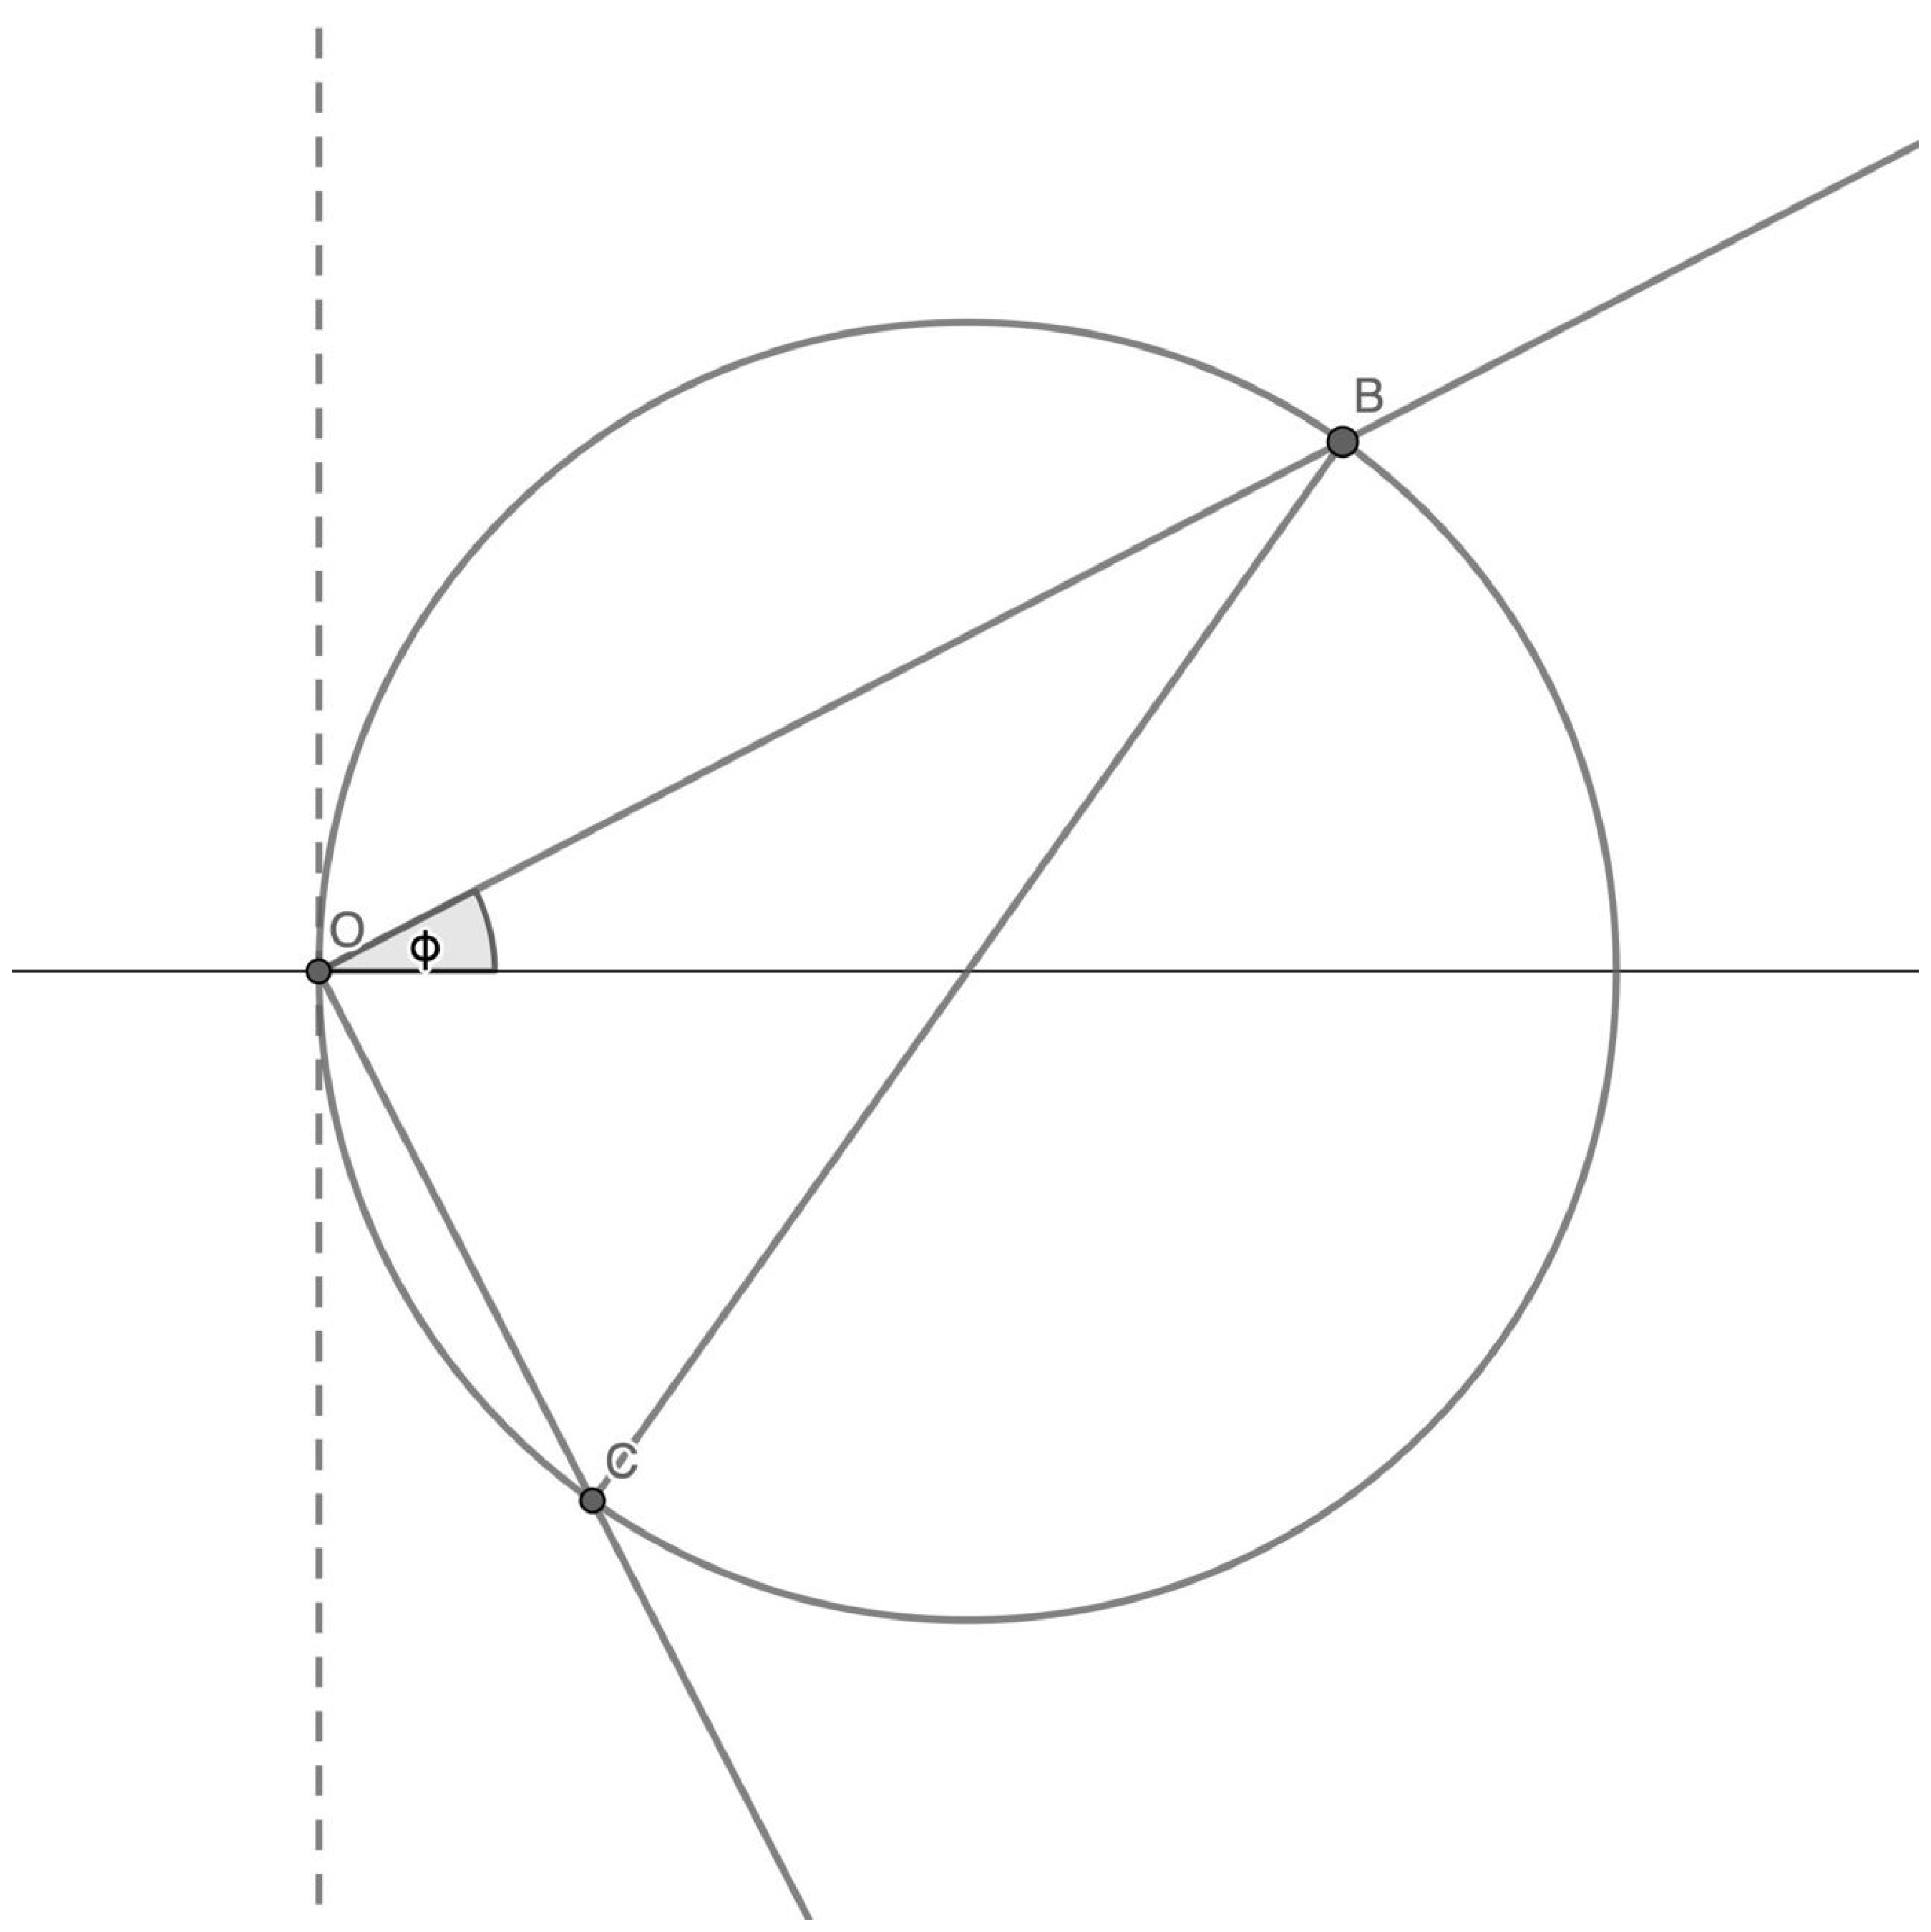
\includegraphics[width=0.5 \linewidth]{isoperimetric_3.eps}}
		\caption{Фокус}
	\end{figure}
	
	Тогда то, что на рисунке отмечено как \(OB\), это не что иное, как \(r(\varphi)\), а \(OC\) --- это \(r \left(\varphi - \dfrac{\pi}{2} \right)\). Но ведь \(OB\) и \(OC\) --- катеты прямоугольного треугольника, а значит \({OB}^2 + {OC}^2 = {BC}^2\). А так как \(BC \leqslant diam \ G \leqslant 1\), то и \(r^2(\varphi) + r^2 \left(\varphi - \dfrac{\pi}{2} \right) \leqslant 1\). А это, в свою очередь, значит, что \[
	\sigma(G) = \frac{1}{2} \int_{0}^{\frac{\pi}{2}} r^2 \left(\varphi - \frac{\pi}{2} \right) +  r^2(\varphi) d\varphi \leqslant \frac{1}{2} \int_{0}^{\frac{\pi}{2}} 1 d\varphi = \frac{\pi}{4}.
	\]
	
	ДОДЕЛАТЬ ПРО ПОЧТИ ДИФФЕРЕНЦИРУЕМОСТЬ (И МБ ПРО ВЫПУКЛЫЙ ПОДГРАФИК)
\end{proof}

\subsection{Обобщённая теорема о плотности}

\hypertarget{plotn}{}
\begin{theorem}
	Пусть \(\Phi \colon Segm \langle a, b \rangle \to \mathbb{R}\) --- аддитивная функция промежутка, функция \(f \colon \langle a, b \rangle \to \mathbb{R}\) непрерывна. Возьмём произвольный отрезок \(\Delta \in Segm \langle a, b \rangle\) и введём следующие обозначения: \(m_\Delta \leqslant \inf\limits_{x \in \Delta} f(x)\) и \(M_\Delta \geqslant \sup\limits_{x \in \Delta} f(x)\). Тогда если выполняются следующие условия:
	\begin{enumerate}
		\item \label{plotn_1} \(m_\Delta |\Delta| \leqslant \Phi(\Delta) \leqslant M_\Delta |\Delta|\),
		\item \label{plotn_2} \(\forall x \in \Delta \quad m_\Delta \leqslant f(x) \leqslant M_\Delta\),
		\item \label{plotn_3} \(\forall \Delta \mid |\Delta| \to 0 \quad M_\Delta - m_\Delta \to 0\)\footnote{То есть в контексте теоремы \(m_\Delta\) --- это слегка заниженный инфимум \(f\), а \(M_\Delta\) --- слегка завышенный супремум \(f\).},
	\end{enumerate}
	то \(f\) --- плотность функции \(\Phi\), то есть \[
	\forall [p, q] \in Segm \langle a, b \rangle \qquad \Phi([p, q]) = \int\limits_p^q f.
	\]
\end{theorem}

\begin{proof}
	Доказательство (как и теорема) очень-очень похоже на доказательство \hyperlink{afp}{теоремы о вычислении аддитивной функции промежутка по плотности}.
	
	Зафиксируем \([p, q] \in Segm \langle a, b \rangle\). Рассмотрим функцию \(F\): \[
	F(x) =
	\begin{cases}
		\Phi([p, x]), & p < x \leqslant q \\
		0,			  & x = p.
	\end{cases}
	\]
	Теперь проверим, что \(F\) --- первообразная \(f\) на \([p, q]\). Имеем: \[
	F'_+(x) = \lim_{h \to +0} \frac{\Phi([p, x + h]) - \Phi([p, x])}{h} = \lim_{h \to +0} \frac{\Phi([x, x + h])}{h}.
	\]
	Согласно пункту~\ref{plotn_1}, \(|\Delta| \cdot m_\Delta \leqslant \Phi(\Delta) \leqslant |\Delta| \cdot M_\Delta\), то есть \(m_\Delta \leqslant \dfrac{\Phi(\Delta)}{|\Delta|} \leqslant M_\Delta\), или
	\begin{equation} \label{plotn_e}
		m_{[x, x + h]} \leqslant \frac{\Phi([x, x + h])}{h} \leqslant M_{[x, x + h]}.
	\end{equation}
	Согласно пункту~\ref{plotn_2}, для всех \(x \) из \(\Delta\) справедливо \(m_\Delta \leqslant f(x) \leqslant M_\Delta\), то есть \(m_{[x, x + h]} \leqslant f(x) \leqslant M_{[x, x + h]}\), или \(-M_{[x, x + h]} \leqslant -f(x) \leqslant -m_{[x, x + h]}\). Сложим это неравенство с неравенством~\eqref{plotn_e}: \[
	m_{[x, x + h]} - M_{[x, x + h]} \leqslant \frac{\Phi([x, x + h])}{h} - f(x) \leqslant M_{[x, x + h]} - m_{[x, x + h]},
	\]
	Наконец, согласно пункту~\ref{plotn_3}, для любого \(\Delta \to [x, x]\) справедливо, что \(M_\Delta - m_\Delta \to 0\), то есть мы можем перейти к пределу: \[
	\lim_{h \to 0} m_{[x, x + h]} - M_{[x, x + h]} \leqslant \lim_{h \to 0} \frac{\Phi([x, x + h])}{h} - f(x) \leqslant \lim_{h \to 0} M_{[x, x + h]} - m_{[x, x + h]}.
	\]
	То есть \(F'_+(x) \to  f(x)\) при \(h \to 0\).
	
	Аналогично \(F'_-(x) = f(x)\). Применим \hyperlink{t9}{формулу Ньютона -- Лейбница} и получим требуемый результат: \[
	\Phi([p, q]) = F(q) - F(p) = \int_p^q f.
	\]
\end{proof}

\subsection{Объём фигур вращения}

\begin{theorem}
	ДОДЕЛАТЬ
\end{theorem}

\begin{proof}
	ДОДЕЛАТЬ
\end{proof}

\subsection{Вычисление длины гладкого пути}

\begin{theorem}
	Пусть \(\gamma \colon [a, b] \to \mathbb{R}^m\) --- гладкий путь, причём инъективный. Тогда \[
	l(\gamma) = \int\limits_a^b ||\gamma'(t)|| dt.
	\]
\end{theorem}

\begin{proof}
	Зафиксируем \(\Delta \in Segm [a, b]\) и рассмотрим функцию \(\Phi\), такую, что \(\Phi(\Delta) = l(\gamma |_\Delta)\). Заметим, что согласно аксиоме~\ref{way2} \(\Phi\) --- аддитивная функция промежутка. Тогда если мы докажем, что функция \(||\gamma'||\) --- плотность \(\Phi\), то, применив \hyperlink{plotn}{\bfseries обобщённую теорему о плотности}, мы докажем нашу теорему.
	
	Для этого мы должны проверить три условия из \hyperlink{plotn}{теоремы}. Сделаем это: для начала нужно предъявить слегка заниженный инфимум (минимум) \(m_\Delta\) и слегка завышенный супремум (максимум) \(M_\Delta\). Введём следующие обозначения:
	\begin{align*}
		m_{i\Delta} = \min\limits_{t \in \Delta} |\gamma'_i (t)|&, &&M_{i\Delta} = \max\limits_{t \in \Delta} |\gamma'_i (t)|, \\
		m_\Delta = \sqrt{\sum\limits_{i = 1}^m m_{i\Delta}^2}&, &&M_\Delta = \sqrt{\sum\limits_{i = 1}^m M_{i\Delta}^2},
	\end{align*}
	
	
	где \(i \in 1 : m\).\footnote{Минимум и максимум достигаются по теореме Вейерштрасса, так как функция \(|\gamma'_i(t)|\) непрерывна как композиция непрерывных функций, а рассматриваем мы её на отрезке.} Теперь начнём проверять необходимые условия:
	\begin{enumerate}
		\item Проверим справедливость верхней границы, справедливость нижней проверяется аналогичным образом. Введём \(\widetilde{\gamma} \colon \Delta \to \mathbb{R}^m\), такой, что \(\widetilde{\gamma}(t) = (M_{1\Delta} \cdot t, M_{2\Delta} \cdot t, \ldots, M_{m\Delta} \cdot t)\). Тогда \(C_{\gamma |_\Delta}\) и \(C_{\widetilde{\gamma}}\) --- носители наших путей. Рассмотрим отображение \(T \colon C_{\gamma |_\Delta} \to C_{\widetilde{\gamma}}\), которое переводит \(\gamma(t)\) в \(\widetilde{\gamma}(t)\). Проверим, что это растяжение: для любых  \(t_0, t_1 \in \Delta\) справедливо \[
		\rho(\gamma(t_0), \gamma(t_1)) =  \sqrt{\sum\limits_{i = 1}^m (\gamma_i (t_0) - \gamma_i (t_1))^2} = \ldots
		\]
		Заметим, что по теореме Лагранжа \[
		\gamma_i (t_0) - \gamma_i (t_1) = \frac{\gamma_i (t_0) - \gamma_i (t_1)}{t_0 - t_1} (t_0 - t_1) = \gamma'_i(c_i) \cdot (t_0 - t_1), \ \text{где} \ c_i \in (t_0, t_1).
		\]
		Продолжим: \[
		\ldots =  \sqrt{\sum\limits_{i = 1}^m (\gamma'_i(c_i) \cdot (t_0 - t_1))^2} \leqslant \sqrt{\sum\limits_{i = 1}^m (M_{i\Delta} (t_0 - t_1) )^2} = \rho(\widetilde{\gamma}(t_0), \widetilde{\gamma}(t_1)).
		\]
		Мы доказали, что \(T\) --- растяжение, а сейчас нам полезно записать результат немного иным образом: для любых \(t_0, t_1 \in \Delta\) справедливо \[
		\rho(\gamma(t_0), \gamma(t_1)) \leqslant \rho(\widetilde{\gamma}(t_0), \widetilde{\gamma}(t_1)) = \sqrt{\sum\limits_{i = 1}^m (M_{i\Delta} (t_0 - t_1) )^2} = M_\Delta |t_0 - t_1|.
		\]
		Теперь мы можем выбрать любое дробление отрезка \(\Delta\) --- пусть \(\eta = \{t_0, t_1, \ldots, t_n\}\) --- и записать для него следующее неравенство: \[
		\sum_{i = 0}^n \rho(\gamma(t_i), \gamma(t_{i + 1})) \leqslant \sum_{i = 0}^n M_\Delta |t_i - t_{i + 1}| = M_\Delta \sum_{i = 0}^n |t_i - t_{i + 1}|.
		\]
		Если перейти к пределу при ранге дробления, стремящемся к нулю, неравенство выглядит так: \[
		\Phi(\Delta) \leqslant M_\Delta |\Delta|,
		\]
		а это как раз то, что мы хотели получить.
		\item Очевидно следует из определения введённых нами \(m_\Delta\) и \(M_\Delta\): при всех \(t \in \Delta\) \[
		m_\Delta \leqslant ||\gamma'(t)||\leqslant M_\Delta.
		\]
		\item Так как при \(|\Delta| \to 0 \ \max\limits_{t \in \Delta} |\gamma'_i (t)| - \min\limits_{t \in \Delta} |\gamma'_i (t)| \to 0\) для всех \(i \in 1 : m\), то и \(M_\Delta - m_\Delta \to 0\).
	\end{enumerate}
\end{proof}

\subsection{Теорема о функциях ограниченной вариации}

\begin{theorem}
	Пусть \(f\colon [a, b] \to \mathbb{R}\) --- \hyperlink{orgvar}{\bfseries функция ограниченной вариации}. Тогда существуют монотонные функции \(p, q\colon [a, b] \to \mathbb{R}\) такие, что для всех \(x \in [a, b]\) \(f(x) = p(x) - q(x)\).
\end{theorem}
\begin{proof}
	Возьмём такие \(p(x), q(x)\), что
	\begin{align*}
		2 \cdot p(x) &= \bigvee_a^x f + (f(x) - f(a)), \\
		2 \cdot q(x) &= \bigvee_a^x f - (f(x) - f(a)).
	\end{align*}
	Тогда имеем равенство \(f(x) - f(a) = p(x) - q(x)\). В принципе, это нам подходит, потому что \(f(a)\) --- константа, и мы можем прибавить её к \(p(x)\) или \(q(x)\), чтобы получить нужное равенство.
	
	Проверим теперь, что \(p\) и \(q\) возрастают, то есть что \(\bigvee_a^x f\) растёт быстрее, чем \(f(x)\). Пусть \(x < y\), запишем \[
	|f(y) - f(x)| \leqslant \bigvee_x^y f.
	\]
	Заметим, что функция \(\Phi\), переводящая \([u, v]\) в \(\bigvee_u^v f\), является аддитивной функцией промежутка (ДОДЕЛАТЬ). Тогда
	\begin{gather*}
		2 \cdot p(y) - 2 \cdot p(x) = \bigvee_x^y f + f(y) - f(x) \geqslant 0, \quad \text{то есть} \quad p(y) \geqslant p(x), \\
		2 \cdot q(y) - 2 \cdot q(x) = \bigvee_x^y f + f(x) - f(y) \geqslant 0, \quad \text{то есть} \quad q(y) \geqslant q(x).
	\end{gather*}
	Ну, вот и всё...
	
	И, \textit{кстати}, \(p(x) + q(x) = \bigvee_a^x f\).
\end{proof}

\subsection{\itshape Интеграл как предел интегральных сумм}

\begin{theorem}
	Пусть функция \(f \colon [a, b] \to \mathbb{R}\) непрерывна. Тогда
	\begin{gather*}
		\forall \varepsilon > 0 \quad \exists \delta > 0 \quad \forall \tau = \{x_i\}_{i = 0}^n \mid \text{ранг} \ \tau < \delta \quad \forall \text{оснащения} \ \{\xi_i\}_{i = 1}^n \ldots \\
		\ldots \left|\sum_{i = 1}^n f(\xi_i) (x_i - x_{i - 1}) - \int\limits_a^b f(x) dx \right| < \varepsilon.
	\end{gather*}
\end{theorem}

\begin{proof}
	Так как \(f\) непрерывна на отрезке, по теореме Кантора она равномерна непрерывна, то есть \[
	\forall \varepsilon > 0 \quad \exists \delta > 0 \quad \forall x_1, x_2 \mid |x_1 - x_2| < \delta \quad |f(x_1) - f(x_2)| < \frac{\varepsilon}{b - a}.
	\]
	Зафиксируем \(\varepsilon\) и подберём соответствующее \(\delta\). Возьмём дробление \(\tau\), ранг которого меньше \(\delta\).
	
	Теперь немного поработаем над нашими интегралом и суммой. Представим интеграл как сумму интегралов по отрезкам \([x_{i - 1}, x_i]\), а слагаемые интегральной суммы \(\sum\limits_{i = 1}^n f(\xi_i) (x_i - x_{i - 1})\) представим как интегралы константы \(f(\xi_i)\) по промежутку \([x_{i - 1}, x_i]\). Получим следующее: \[
	\sum_{i = 1}^n \int_{x_{i - 1}}^{x_i} f(\xi_i) dx - \sum_{i = 1}^n \int_{x_{i - 1}}^{x_i} f(x) dx = \sum_{i = 1}^n \int_{x_{i - 1}}^{x_i} f(\xi_i) - f(x) dx.
	\]
	То есть имеем \[
	\left|\sum_{i = 1}^n \int_{x_{i - 1}}^{x_i} f(\xi_i) - f(x) dx \right| \leqslant \sum_{i = 1}^n \int_{x_{i - 1}}^{x_i} \left|f(\xi_i) - f(x) \right| dx \leqslant \ldots
	\]
	Так как мы подобрали дробление с таким рангом, что для всех \(x \in [x_{i - 1}, x_i]\) и для любого оснащения \(\{\xi_i\}_{i = 1}^n \ |f(\xi_i) - f(x)| < \dfrac{\varepsilon}{b - a}\), можем продолжить цепочку неравенств: \[
	\ldots \leqslant \sum_{i = 1}^n \int_{x_{i - 1}}^{x_i} \frac{\varepsilon}{b - a} dx = \int\limits_a^b \frac{\varepsilon}{b - a} dx = \varepsilon.
	\]
\end{proof}

\subsection{Теорема об интегральных суммах центральных прямоугольников и трапеций}

\hypertarget{trap}{}
\begin{theorem}
	Пусть \(f \in C^2 [a, b]\), \(\tau = \{x_i\}_{i = 0}^n\) --- дробление отрезка \([a, b]\) с рангом \(\delta\). Выберем оснащение \(\{\xi_i\}_{i = 1}^n\), где \(\xi_i = \dfrac{x_i + x_{i - 1}}{2}\). Тогда справедливы следующие утверждения:
	\begin{gather}
		\label{intsum1}
		\left|\int\limits_a^b f(x) dx - \sum_{i = 1}^n f(\xi_i) (x_i - x_{i - 1}) \right| \leqslant \frac{\delta^2}{8} \int\limits_a^b |f''(x)| dx, \\
		\label{intsum2}
		\left|\int\limits_a^b f(x) dx - \sum_{i = 1}^n \frac{f(x_i) + f(x_{i - 1})}{2} (x_i - x_{i - 1})\right| \leqslant \frac{\delta^2}{8} \int\limits_a^b |f''(x)| dx.
	\end{gather}
\end{theorem}

\begin{proof}[Доказательство неравенства~\eqref{intsum2}]
	Рассмотрим интеграл на отрезке дробления и преобразуем его: \[
	\int_{x_{i - 1}}^{x_i} f(x) dx = \int_{x_{i - 1}}^{x_i} f(x) d(x - \xi_i) = \ldots
	\]
	Проинтегрируем его по частям: \[
	\ldots = f(x) (x - \xi_i) \bigg|_{x_{i - 1}}^{x_i} - \int_{x_{i - 1}}^{x_i} f'(x) (x - \xi_i) dx = \ldots
	\]
	Воспоминаем, что \(\xi_i = \dfrac{x_i + x_{i - 1}}{2}\): \[
	\ldots = \frac{f(x_i) + f(x_{i - 1})}{2} (x_i - x_{i - 1}) - \int_{x_{i - 1}}^{x_i} f'(x) (x - \xi_i) dx = \ldots
	\]
	Введём функцию \(\psi(x) = (x_i - x) (x - x_{i - 1})\) и рассмотрим её производную \(\psi'(x) = -(x - x_{i - 1}) + (x_i - x) = -2x + x_{i - 1} + x_i\). Заметим, что \(-\dfrac{1}{2} \psi'(x) = x - \xi_i\). Тогда продолжим: \[
	\ldots = \frac{f(x_i) + f(x_{i - 1})}{2} (x_i - x_{i - 1}) + \frac12 \int_{x_{i - 1}}^{x_i} f'(x) \cdot \psi'(x) dx = \ldots
	\]
	Опять проинтегрируем по частям:
	\begin{gather*}
		\ldots = \frac{f(x_i) + f(x_{i - 1})}{2} (x_i - x_{i - 1}) + \ldots \\
		\ldots + \frac{f'(x) \cdot \psi(x)}{2} \bigg|_{x_{i - 1}}^{x_i} - \frac{1}{2}\int_{x_{i - 1}}^{x_i} f''(x) \cdot \psi(x) dx = \ldots \\
		\ldots = \frac{f(x_i) + f(x_{i - 1})}{2} (x_i - x_{i - 1}) - \frac{1}{2}\int_{x_{i - 1}}^{x_i} f''(x) \cdot \psi(x) dx
	\end{gather*}
	
	Начнём разбираться с нашим неравенством:
	\begin{gather*}
		\left|\int\limits_a^b f - \sum_{i = 1}^n \textit{слагаемое}_i \right| = \left|\sum_{i = 1}^n \int_{x_{i - 1}}^{x_i} f - \sum_{i = 1}^n \textit{слагаемое}_i \right| = \ldots \\
		\ldots = \left|\sum_{i = 1}^n \int_{x_{i - 1}}^{x_i} f - \textit{слагаемое}_i \right| \leqslant \sum_{i = 1}^n \left|\int_{x_{i - 1}}^{x_i} f - \textit{слагаемое}_i \right|.
	\end{gather*}
	Воспользуемся нашими наработками:
	\begin{gather*}
		\sum_{i = 1}^n \left|\frac{f(x_i) + f(x_{i - 1})}{2} (x_i - x_{i - 1}) - \frac{1}{2}\int_{x_{i - 1}}^{x_i} f''(x) \cdot \psi(x) dx - \textit{слагаемое}_i \right| = \ldots \\
		\ldots = \frac{1}{2} \sum_{i = 1}^n \left|\int_{x_{i - 1}}^{x_i} f''(x) \cdot \psi(x) dx \right| \leqslant \frac{1}{2} \sum_{i = 1}^n \int_{x_{i - 1}}^{x_i} \left|f''(x) \cdot \psi(x) \right| dx = \ldots \\
		\ldots = \frac{1}{2} \int_a^b \left|f''(x) \cdot \psi(x) \right| dx.
	\end{gather*}
	
	Теперь оценим \(\psi(x)\). Рассмотрим \(\psi(\xi_i) = (x_i - \xi_i) (\xi_i - x_{i - 1})\): \[
	\psi(\xi_i) = \left(x_i - \frac{x_i + x_{i - 1}}{2} \right) \left(\frac{x_i + x_{i - 1}}{2} - x_{i - 1}\right) = \left(\frac{x_i - x_{i - 1}}{2} \right)^2.
	\]
	Так как ранг дробления \(\tau\) равен \(\delta\), справедливо: \[
	\psi(\xi_i) \leqslant \frac{\delta^2}{4}.
	\]
	Тогда \[
	\frac{1}{2} \int_a^b \left|f''(x) \cdot \psi(x) \right| dx \leqslant \frac{\delta^2}{8} \int_a^b \left|f''(x) \right| dx.
	\]
\end{proof}

\subsection{Формула Эйлера -- Маклорена, асимптотика степенных сумм}

\hypertarget{eumak}{}
\begin{theorem}
	Пусть \(f \in C^2 [m, n]\), где \(m, n \in \mathbb{Z}\). Тогда \[
	\int\limits_m^n f(x) dx = \sum\limits_{i = m}^n f(i) - \frac{1}{2} \int\limits_m^n f''(x) \{x\} (1 - \{x\}) dx,
	\]
	\textbf{причём} первое и последнее слагаемые в сумме \(\sum\limits_{i = m}^n f(i)\) входят в неё с весом $\dfrac{1}{2}$.
\end{theorem}

\begin{proof}
	В процессе доказательства \hyperlink{trap}{формулы трапеций} мы установили (сразу перед итоговой оценкой через \(\delta\)), что \[
	\int\limits_a^b f(x) dx - \sum_{i = 1}^n \frac{f(x_i) + f(x_{i - 1})}{2} (x_i - x_{i - 1}) = -\frac{1}{2} \int_a^b f''(x) \cdot \psi(x) dx
	\]
	(у правой части здесь опять появляется минус, который в прошлой теореме был съеден модулем). Выберем дробление на отрезки вида \([i - 1, i]\), где \(i \in (m + 1) : n\). Тогда
	\begin{gather*}
		\sum_{i = 1}^n \frac{f(x_i) + f(x_{i - 1})}{2} (x_i - x_{i - 1}) = \sum_{i = m + 1}^n \frac{f(i - 1) + f(i)}{2} = \ldots \\
		\ldots = \frac{f(m)}{2} + \frac{f(m + 1)}{2} + \frac{f(m + 1)}{2} + \ldots + \frac{f(n - 1)}{2} + \frac{f(n)}{2} = \sum\limits_{i = m}^n f(i),
	\end{gather*}
	причём первое и последнее слагаемые входят в сумму с весом \(\dfrac{1}{2}\), как нам и нужно.
	
	Теперь вспомним, что \(\psi(x) = (x_i - x) (x - x_{i - 1})\). Так как в нашем случае \(x_i\) и \(x_{i - 1}\) --- это соседние целые числа, получаем как раз \(\psi(x) = \{x\} (1 - \{x\})\). Теорема доказана, осталось только всё красиво записать.
\end{proof}

\begin{example}
	\[
	1^p + 2^p + \ldots + n^p = \frac{n^p}{2} + \frac{n^{p + 1}}{p + 1} + O(\max(1, n^{p - 1})) \enskip  \text{при} \ p > -1.
	\]
\end{example}

\begin{proof}
	Рассмотрим \(f(x) = x^p\). По \hyperlink{eumak}{формуле Эйлера -- Маклорена}\[
	1^p + 2^p + \ldots + n^p = \int_1^n x^p dx + \frac{1}{2} + \frac{n^p}{2} + \frac{p (p - 1)}{2} \int_1^n x^{p - 2} \{x\} (1 - \{x\}) dx.
	\]
	Возьмём интеграл \(x^p\): \[
	\int_1^n x^p dx = \frac{n^{p + 1} - 1}{p + 1}
	\]
	и оценим второй интеграл: \[
	0 \leqslant \int_1^n x^{p - 2} \{x\} (1 - \{x\}) dx \leqslant \frac{1}{4} \cdot \left(\frac{n^{p - 1} - 1}{p - 1} \right).
	\]
	Справедливость нижней границы очевидна, так как мы рассматриваем положительные \(x\), а справедливость верхней следует из того, что максимум функции \(\{x\} (1 - \{x\})\) достигается в точке \(x = \dfrac{1}{2}\), так как это, как говорилось выше, лишь частный случай функции \(\psi(x) = (x_i - x) (x - x_{i - 1})\), где \(x_i\) и \(x_{i - 1}\) --- соседние целые числа.
	
	Понятно, что при при \(p > 1\) правая часть превращается в \(O(n^{p - 1})\), а при \(-1 < p < 1\) --- в \(O(1)\), тогда наш интеграл --- \(O(\max(1, n^{p - 1}))\). Отметим, что при \(p = 1\), рассуждения заканчиваются в самом начале, так как  \(\dfrac{p (p - 1)}{2} = 0\). Закинем под \(O\) все имеющиеся константы и получим, что нужно.
\end{proof}

\subsection{Асимптотика частичных сумм гармонического ряда}

\begin{example}
	\[
	1 + \frac{1}{2} + \frac{1}{3} + \ldots + \frac{1}{n} = \ln n + \gamma + o(1) \enskip \text{при} \ \gamma \in \left[\frac{4}{8}, \frac{5}{8}\right].
	\]
\end{example}

\begin{proof}
	Рассмотрим \(f(x) = \dfrac{1}{x}\). По \hyperlink{eumak}{формуле Эйлера -- Маклорена} \[
	1 + \frac{1}{2} + \frac{1}{3} + \ldots + \frac{1}{n} = \int_1^n \frac{1}{x} dx + \frac{1}{2} + \frac{1}{2n} + \int_1^n \frac{1}{x^3} \{x\} (1 - \{x\}) dx.
	\] 
	Как и в прошлый раз, возьмём интеграл \(\dfrac{1}{x}\): \[
	\int_1^n \frac{1}{x} dx = \ln n.
	\]
	Заметим, что второй интеграл возрастает при увеличении \(n\) (подынтегральное выражение положительно, а промежуток интегрирование увеличивается) и оценим его: \[
	0 \leqslant \int_1^n \frac{1}{x^3} \{x\} (1 - \{x\}) dx \leqslant \frac{1}{4} \left(-\frac{1}{2n^2} + \frac{1}{2} \right) = \frac{1}{8} \left(1 - \frac{1}{n^2} \right) \leqslant \frac{1}{8}.
	\]
	Так как имеющаяся у нас $\dfrac{1}{2n}$ стремится к нулю при \(n \to \infty\), получаем: \[
	1 + \frac{1}{2} + \frac{1}{3} + \ldots + \frac{1}{n} = \ln n + \gamma + o(1).
	\]
	В константу \(\gamma\) мы записали \(\dfrac{1}{2}\) и значение интеграла, то есть \(\gamma \in \left[\dfrac{4}{8}, \dfrac{5}{8}\right]\), а \(o(1)\) --- это \(\dfrac{1}{2n}\), стремящаяся к нулю при \(n \to \infty\).
\end{proof}

\begin{remark}
	Константа \(\gamma\) называется \textit{постоянной Эйлера} и равняется примерно \(0,577\ldots\)
\end{remark}

\subsection{Формула Валлиса}

\hypertarget{vallem}{}
\begin{lemma}
	Если \(n \in \mathbb{Z}_+\), то \[
	\int_0^{\frac{\pi}{2}} \sin^n x \, dx = \frac{(n - 1)!!}{n!!} \cdot
	\begin{cases}
		\dfrac{\pi}{2}, &\text{если \(n\) чётно}, \\
		1, 				&\text{если \(n\) нечётно}.
	\end{cases}
	\]
\end{lemma}

\begin{proof}
	Обозначим \(I_n = \displaystyle\int_0^{\frac{\pi}{2}} \sin^n x \, dx\). Легко проверить, что \(I_0 = \dfrac{\pi}{2}, \ I_1 = 1\). При \(n - 1 \in \mathbb{N}\) проинтегрируем по частям:
	\begin{multline*}
		I_n = \int_0^{\frac{\pi}{2}} \sin^n x \, dx = \int_0^{\frac{\pi}{2}} \sin^{n - 1} x \, d(-\cos x) = -\sin^{n - 1} x \, \cos x \bigg|_0^{\frac{\pi}{2}} + \\ 
		+ (n - 1) \int_0^\frac{\pi}{2} \sin^{n - 2} x \, \cos^2 x \, dx.
	\end{multline*}
	Учтём, что двойная подстановка обнуляется, и применим формулу \linebreak \(\cos^2 x = 1 - \sin^2 x\)):
	\begin{multline*}
		I_n = (n - 1) \left(\int_0^\frac{\pi}{2} \sin^{n - 2} x \, dx - \int_0^\frac{\pi}{2} \sin^n x \, dx \right) = (n - 1) (I_{n - 2} - I_n).
	\end{multline*}
	Выражая \(I_n\), получим рекуррентное соотношение \[
	I_n = \frac{n - 1}{n} I_{n - 2}.
	\]
	Теперь, применив его несколько раз, мы можем выразить \(I_n\) через \(I_0\), если \(n\) чётно, или через \(I_1\), если \(n\) нечётно. Чётность/нечётность числителя и знаменателя будет сохраняться.
\end{proof}

\hypertarget{wall}{}
\begin{theorem}
	\[
	\pi = \lim_{n \to \infty} \frac{1}{n} \left(\frac{(2n)!!}{(2n - 1)!!} \right)^2.
	\]
\end{theorem}
\begin{proof}
	При всех \(x \in \left(0, \dfrac{\pi}{2} \right)\) выполняется неравенство \linebreak \(0 < \sin x < 1\), поэтому для любого \(n \in \mathbb{N}\) \[
	\sin^{2n + 1} x < \sin^{2n} x < \sin^{2n - 1} x,
	\]
	а тогда и \[
	I_{2n + 1} < I_{2n} < I_{2n - 1}.
	\]
	Применяя \hyperlink{vallem}{лемму}, получаем двойное неравенство \[
	\frac{(2n)!!}{(2n + 1)!!} < \frac{(2n - 1)!!}{(2n)!!} \cdot \frac{\pi}{2} < \frac{(2n - 2)!!}{(2n - 1)!!},
	\]
	что равносильно \[
	\frac{1}{2n + 1} \left(\frac{(2n)!!}{(2n - 1)!!} \right)^2 < \frac{\pi}{2} < \frac{1}{2n} \left(\frac{(2n)!!}{(2n - 1)!!} \right)^2.
	\]
	Обозначим \(x_n = \dfrac{1}{n} \left(\dfrac{(2n)!!}{(2n - 1)!!} \right)^2\). Двойное неравенство принимает вид \[
	\frac{n}{2n + 1} x_n < \frac{\pi}{2} < \frac{1}{2} x_n.
	\]
	Из правой части получаем, что \(\pi < x_n\), из левой --- что \(x_n < \dfrac{2n + 1}{2n} \pi\). Отсюда имеем \(x_n \xrightarrow[n \to \infty]{} \pi\).
\end{proof}

\subsection{\itshape Формула Стирлинга}

\begin{theorem}
	\[
	n! \sim n^n \, e^{-n} \, \sqrt{2\pi n} \enskip \textit{при} \ n \to \infty.
	\]
\end{theorem}

\begin{proof}
	Рассмотрим \(f(x) = \ln x\). По \hyperlink{eumak}{формуле Эйлера -- Маклорена} \[
	\ln 1 + \ln 2 + \ldots + \ln n = \int_1^n \ln x \, dx + \frac{\ln n}{2} - \frac{1}{2} \int_1^n \frac{1}{x^2} \{x\} (1 - \{x\}) \, dx.
	\]
	Интегрированием по частям находим \(\displaystyle\int_1^n \ln x \, dx = n \ln n - n + 1\). Заметим, что второй интеграл возрастает с увеличением \(n\) и оценим его: \[
	0 \leqslant \int_1^n \frac{1}{x^2} \{x\} (1 - \{x\}) \, dx \leqslant \frac{1}{4} \left(1 - \frac{1}{n} \right) \leqslant \frac{1}{4}.
	\]
	Получаем \[
	\ln 1 + \ln 2 + \ldots + \ln n = n \ln n - n + \frac{\ln n}{2} + C + o(1).
	\]
	В константу \(C + o(1)\) мы записали \(1\) и значение интеграла, \(o(1)\) отражает погрешность.
	
	Так как \(\ln 1 + \ln 2 + \ldots + \ln n = \ln(n!)\), возьмём от этого всего экспоненту и получим \[
	n! = n^n e^{-n} \sqrt{n} \, e^{C + o(1)}.
	\]
	Выражение \(e^{C + o(1)}\) стремится к какой-то константе, которую мы обозначим за \(C'\). Выясним, чему она равна. Из \hyperlink{wall}{формулы Валлиса} имеем \[
	\sqrt{\pi} = \lim_{n \to \infty} \frac{1}{\sqrt{n}} \cdot \frac{(2n)!!}{(2n - 1)!!}.
	\]
	Преобразуем эту формулу: \[
	\frac{1}{\sqrt{n}} \cdot \frac{(2n)!!}{(2n - 1)!!} = \frac{1}{\sqrt{n}} \cdot \frac{2^n \cdot n!}{(2n - 1)!!} = \frac{1}{\sqrt{n}} \cdot \frac{2^n \cdot n! \cdot (2n)!!}{(2n)!} = \frac{(2^n \cdot n!)^2}{\sqrt{n} \cdot (2n)!}.
	\]
	Теперь можем воспользоваться нашими наработками: \[
	\frac{(2^n \cdot n!)^2}{\sqrt{n} \cdot (2n)!} = \frac{(2^n \cdot n^n e^{-n} \sqrt{n} \, C')^2}{\sqrt{n} \cdot (2n)^{2n} e^{-2n} \sqrt{2n} \, C'} = \frac{C'}{\sqrt{2}}.
	\]
	То есть \(\sqrt{\pi} = \lim\limits_{n \to \infty} \dfrac{C'}{\sqrt{2}} = \dfrac{C'}{\sqrt{2}}\), откуда \(C' = \sqrt{2\pi}\) и \(n! = n^n e^{-n} \sqrt{2\pi n}.\) 
	
\end{proof}

\subsection{Три леммы о сверхограниченных множествах}

\begin{lemma}
	Множество \(D\) сверхограниченно в \(X\) тогда и только тогда, когда \(D\) сверхограниченно в себе.
\end{lemma}

\begin{proof}
	Достаточность очевидна, докажем необходимость.
	
	Построим множество \(E_X = \{x_0, x_1,\ldots, x_n\} \subset X\) --- конечную \(\dfrac{\varepsilon}{2}\)-сеть для \(D\). То есть имеем: \[
	\forall y \in D \quad \exists x_i \in E_X \quad \rho(x, y) < \frac{\varepsilon}{2}.
	\]
	В кажом шаре \(B_{\frac{\varepsilon}{2}} (x_i)\) выберем какое-нибудь \(y_i\). Тогда множество \linebreak \(E_Y = \{y_0, y_1,\ldots, y_m\} \subset D\), где \(m \leqslant n\), --- \(\varepsilon\)-сеть для \(D\), так как \[
	\forall y \in D \quad \exists y_i \in E_Y \quad \rho(y, y_i) \leqslant \rho(y_i, x_i) + \rho(x_i, y) < \varepsilon.
	\]
\end{proof}

\begin{lemma}
	Сверхограниченность сохраняется при равномерно непрерывном отображении.
\end{lemma}

\begin{proof}
	Пусть \(f\) --- равномерно непрерывное отображение. Запишем, что это значит: \[
	\forall \varepsilon > 0 \quad \exists \delta > 0 \quad \forall x, x_i \in D \quad \rho(x, x_i) < \delta \quad \rho(f(x), f(x_i)) < \varepsilon.
	\]
	А из этого напрямую следует, что если мы возьмём \(\delta\)-сеть для \(D\), то её образ будет являться \(\varepsilon\)-сетью для \(f(D)\).
\end{proof}

\begin{lemma}
	Если \(D\) сверхограниченно, то и его замыкание \(Cl(D)\) сверхограниченно.
\end{lemma}

\begin{proof}
	ДОДЕЛАТЬ
\end{proof}

\begin{lemma}
	Множество \(D\) сверхограниченно тогда и только тогда, когда любая последовательность из \(D\) содержит фундаментальную подпоследовательность.
\end{lemma}

\begin{proof}
	Докажем необходимость и достаточность:
	\begin{enumerate}
		\item[\(\Rightarrow\)] Вспомним определение фундаментальной подпоследовательности: \[
		\forall \varepsilon > 0 \quad \exists N \quad \forall n, m > N \quad \rho(y_{n}, y_{m}) < \varepsilon.
		\]
		Построим \(E = \{x_0, x_1,\ldots, x_n\}\) ---  \(\frac{\varepsilon}{2}\)-сеть для \(D\). Рассмотрим последовательность \((y_n)\). Так как наша сеть конечная, понятно, что в каком-то шаре \(B_\varepsilon (x_i)\) содержится бесконечно много членов последовательности. Но тогда расстояние между ними всеми меньше \(\varepsilon\), а значит они и составляют искомую подпоследовательность.
		\item[\(\Leftarrow\)] Пусть для какого-то \(\varepsilon\) не существует конечной \(\varepsilon\)-сети. Тогда есть такая последовательность, что в каждом шаре содержится только конечное число её членов. А из этого напрямую следует отрицание определения фундаментальной последовательности: \[
		\forall N \quad \exists n, m > N \quad \rho(y_{n}, y_{m}) \geqslant \varepsilon.
		\]
	\end{enumerate}
\end{proof}

\subsection{Компактность и конечные эпсилон-сети}

\begin{theorem}
	Пусть \(D \subset X\), где \(X\) --- полное метрическое пространство. Тогда следующие утверждения равносильны:
	\begin{enumerate}
		\item \(D\) компактно,
		\item \(D\) сверхограниченно и замкнуто.
	\end{enumerate}
\end{theorem}

\begin{proof}
	Докажем необходимость и достаточность:
	\begin{enumerate}
		\item[\(\Rightarrow\)] В метрическом пространстве компактность равносильна секвенциальной компактности. То есть из любой последовательности мы можем извлечь сходящуюся, а значит, и фундаментальную, подпоследовательность, что равносильно сверхограниченности. Замкнутость следует из компактности.
		\item[\(\Leftarrow\)] Так как \(D\) сверхограниченно, любая последовательность содержит фундаментальную подпоследовательность, которая в силу полноты \(X\) сходится к элементу из \(X\). То есть из любой последовательности мы можем извлечь сходяющуся подпоследовательность, что означает секвенциальную компактность \(D\), которая в метрическом пространстве равносильна компактности.
	\end{enumerate}
\end{proof}

\subsection{Простейшие свойства несобственного интеграла}

\hypertarget{svva}{}
\begin{theorem}
	Пусть функция \(f \colon [a, b) \to \mathbb{R}\) допустима. Тогда:
	\begin{enumerate}
		\item Для любого \(c \in (a, b)\) сходимость \(\int_a^{\to b} f\) равносильна сходимости \(\int_c^{\to b} f\) и, если интегралы сходятся, \[
		\int_a^{\to b} f = \int_a^c f + \int_c^{\to b} f.
		\]
		\item Если \(g\) допустима, интегралы \(\int_a^{\to b} f\) и \(\int_a^{\to b} g\) сходятся, то для любого \(\lambda \in \mathbb{R}\) интегралы \(\int_a^{\to b} \lambda f\) и \(\int_a^{\to b} f \pm g\) также сходятся, причём:
		\begin{enumerate}
			\item \(\displaystyle\int_a^{\to b} \lambda f = \lambda \displaystyle\int_a^{\to b} f\),
			\item \(\displaystyle\int_a^{\to b} f \pm g = \displaystyle\int_a^{\to b} f \pm \displaystyle\int_a^{\to b} g\).
		\end{enumerate}
		\item Если \(g\) допустима, интегралы \(\int_a^{\to b} f\) и \(\int_a^{\to b} g\) существуют в \(\overline{\mathbb{R}}\) (необязательно сходятся) и \(f \leqslant g\) на \([a, b)\), то \[
		\int_a^{\to b} f \leqslant \int_a^{\to b} g.
		\]
		\item Если \(f, g\) дифференцируемы на \([a, b)\) и \(f', g'\) допустимы, то \[
		\int_a^{\to b} f'g = fg \bigg|_a^{\to b} - \int_a^{\to b} fg'.
		\]
		Это надо понимать так: если существуют два конечных предела из трёх, то третий предел также существует и конечен, причём имеет место вышеизложенное равенство.
		\item Если \(\varphi \colon [\alpha, \beta) \to \langle A, B \rangle\), \(\varphi'\) допустима, то \[
		\int_a^{\to b} f(\varphi) \varphi' = \int_{\varphi(\alpha)}^{\varphi(\beta-)} f.
		\]
		Это надо понимать так: если существует один из интегралов, то существует и другой и имеет место вышеизложенное равенство.
	\end{enumerate}
\end{theorem}

\begin{proof}
	Все свойства доказываются почти одинаковым образом.
	\begin{enumerate}
		\item Для любого \(A \in (c, b)\) по свойству аддитивности определённого интеграла \[
		\int_a^A f = \int_a^c f + \int_c^A f.
		\]
		При \(A \to b-\) предел обеих частей равенства существует или нет одновременно. Перейдём к пределу и получим, что требуется.
		\item Для любого \(A \in [a, b)\) по свойству линейности определённого интеграла \[
		\int_a^A f \pm g = \int_a^A f \pm \int_a^A g \qquad \text{и} \qquad \int_a^A \lambda f = \lambda \int_a^A f.
		\]
		Тогда соответствующие интегралы сходятся, а после предельного перехода получаются необходимые равенства.
		\item Для любого \(A \in [a, b)\) из интегрирования неравенств \[
		\int_a^A f \leqslant\int_a^A g.
		\]
		Перейдём к пределу и получим, что нужно.
		\item Для любого \(A \in [a, b)\) справедливо \[
		\int_a^A f'g = fg \bigg|_a^A - \int_a^A fg'.
		\]
		Сделаем предельный переход и посмотрим, что вышло.
		\item Не будем доказывать, потому что тогда придётся всё аккуратно расписывать, а мы не хотим.
	\end{enumerate}
\end{proof}

\begin{remark}
	Так как мы только что убедились, что свойства несобственного интеграла один в один похожи на свойства определённого, \textit{стрелочку} писать больше \textit{не будем}.
\end{remark}

\subsection{\itshape Признаки сравнения сходимости несобственного интеграла}

\hypertarget{srshlem}{}
\begin{lemma}
	Пусть функция \(f\) допустима на \([a, b)\), \(f \geqslant 0\). Обозначим \linebreak \(\Phi(A) = \displaystyle\int_a^A f(x) \, dx\), где \(A \in [a, b)\). Тогда следующие утверждения равносильны:
	\begin{enumerate}
		\item \(\displaystyle\int_a^b f(x) \, dx\) сходится,
		\item \(\Phi(A)\) ограничена.
	\end{enumerate}
\end{lemma}

\begin{proof}
	Нужно проверить, что конечный предел \(\lim\limits_{A \to b-} \Phi(A)\) существует тогда и только тогда, когда \(\Phi(A)\) ограничена. Понятно, что если предел существует, то функция ограничена. Также очевидно, что \(\Phi(A)\) возрастает. Значит, по теореме о пределе монотонной функции, её предел существует и конечен. 
\end{proof}

\hypertarget{priz}{}
\begin{theorem}
	Пусть функции \(f, g\) допустимы на \([a, b)\), \(f, g \geqslant 0\). Тогда справедливы утверждения:
	\begin{enumerate}
		\item Пусть \(f \leqslant g\) на \([a, b)\). Тогда:
		\begin{enumerate}
			\item \(\int_a^b g\) сходится \(\Rightarrow\) \(\int_a^b f\) сходится,
			\item \(\int_a^b f\) расходится \(\Rightarrow\) \(\int_a^b g\) расходится.
		\end{enumerate}
		\item Пусть \(\lim\limits_{x \to b-} \dfrac{f(x)}{g(x)} = l\). Тогда:
		\begin{enumerate}
			\item Если \(l = +\infty\), то:
			\begin{enumerate}
				\item \(\int_a^b f\) сходится \(\Rightarrow\) \(\int_a^b g\) сходится,
				\item \(\int_a^b g\) расходится \(\Rightarrow\) \(\int_a^b f\) расходится.
			\end{enumerate}
			\item Если \(l = 0\), то:
			\begin{enumerate}
				\item \(\int_a^b g\) сходится \(\Rightarrow\) \(\int_a^b f\) сходится,
				\item \(\int_a^b f\) расходится \(\Rightarrow\) \(\int_a^b g\) расходится.
			\end{enumerate}
			\item Если \(l \in (0, +\infty)\), то \(\int_a^b f\) и \(\int_a^b g\) сходятся и расходятся одновременно.
		\end{enumerate}
	\end{enumerate}
\end{theorem}

\begin{proof}
	Докажем утверждения, которые мы наплодили.
	\begin{enumerate}
		\item Очевидно следует из \hyperlink{srshlem}{леммы}.
		\item
		\begin{enumerate}
			\item Если \(\lim\limits_{x \to b-} \dfrac{f(x)}{g(x)} = +\infty\), то, НСНМ, \(g \leqslant f\). Отсылаем к пункту~1.
			\item Если \(\lim\limits_{x \to b-} \dfrac{f(x)}{g(x)} = 0\), то, НСНМ, \(f \leqslant g\). Опять отсылаем к пункту~1.
			\item Существует такое \(c \in [a, b)\), что для всех \(x \in [c, b)\) выполняется, 	например, \[
			\frac{1}{2} \, l < \frac{f(x)}{g(x)} < \frac{3}{2} \, l,
			\]
			то есть \[
			\frac{1}{2} \, l  \cdot g(x) < f(x) < \frac{3}{2} \, l \cdot g(x).
			\]
			Учитывая, что сходимость на \([a, b)\) равносильна сходимости на \([c, b)\), по пункту~1 из правой части получаем, что если \(\int_a^b g\) сходится, то и \(\int_a^b f\) сходится, а из левой --- что если \(\int_a^b f\) сходится, то и \(\int_a^b g\) сходится. Получили равносильность.
		\end{enumerate}
	\end{enumerate}
\end{proof}

\subsection{Изучение сходимости интеграла $\int_{10}^\infty dx/(x^\alpha (\ln x)^\beta)$}

\begin{example}
	Исследуем интеграл $\displaystyle \int_{10}^{+\infty} \frac{dx}{x^\alpha (\ln x)^\beta}$ на сходимость.
	
	Рассмотрим, как на сходимость влияет \(\alpha\):
	\begin{enumerate}
		\item Пусть \(\alpha > 1\). Запишем \(\alpha = 1 + 2a\), где \(a > 0\). Тогда \[
		\frac{1}{x^\alpha (\ln x)^\beta} = \frac{1}{x^{1+a}} \cdot \frac{1}{x^a (\ln x)^\beta}.
		\]
		Ясно, что \(\dfrac{1}{x^a (\ln x)^\beta} \to 0\) при \(x \to \infty\). Почему? При положительном \(a\) выражение \(x^a \to \infty\) при \(x \to \infty\), а логарифм не сможет этому помешать: при \(\beta \geqslant 0\) он тоже стремится к бесконечности, а при \(\beta < 0\) логарифм просто недостаточно быстро растёт --- проверить это можно, вычислив по \hyperlink{t3}{правилу Лопиталя} \(\lim\limits_{x \to \infty} \dfrac{(\ln x)^{-\beta}}{x^a} = \lim\limits_{x \to \infty} \left(\dfrac{\ln x}{x^{-\frac{a}{\beta}}} \right)^{-\beta}\).
		Тогда, НСНМ, \[
		\frac{1}{x^{1 + a}} \cdot \frac{1}{x^a (\ln x)^\beta} \leqslant 	\frac{1}{x^{1 + a}}.
		\]
		Интеграл \(\displaystyle \int_{10}^{+\infty} \frac{1}{x^{1 + a}}\) сходится как \hyperlink{etint}{эталонный}, а значит и рассматриваемый интеграл тоже сходится.
		\item Пусть теперь \(\alpha < 1\). Запишем \(\alpha = 1 - 2b\), где \(b > 0\). Тогда \[
		\frac{1}{x^\alpha (\ln x)^\beta} = \frac{1}{x^{1 - b}} \cdot \frac{x^b}{(\ln x)^\beta}.
		\]
		Интеграл от \(\dfrac{1}{x^{1 - b}}\) расходится, а \(\dfrac{x^b}{(\ln x)^\beta}\) этому не мешает, так как стремится к бесконечности при \(x \to \infty\) (опять потому что логарифм растёт медленнее степенной функции).
		Тогда, НСНМ, \[
		\frac{1}{x^\alpha (\ln x)^\beta} \geqslant \frac{1}{x^{1 - b}}.
		\]
		Интеграл \(\displaystyle \int_{10}^{+\infty} \frac{1}{x^{1 - b}}\) расходится как эталонный, а значит и рассматриваемый интеграл тоже расходится.
		\item Пусть \(\alpha = 1\), то есть мы исследуем интеграл \[
		\int_{10}^\infty \frac{dx}{x (\ln x)^\beta}
		\]
		Сделаем замену \(y = \ln x\): \[
		\int_{\ln 10}^{+\infty} \frac{d(e^y)}{e^y y^\beta} = \int_{\ln 10}^{+\infty} \frac{d(y)}{y^\beta}.
		\]
		Это эталонный интеграл, а значит он сходится при  \(\beta > 1\) и расходится при  \(\beta \leqslant 1\).
	\end{enumerate}
\end{example}

\subsection{Интеграл Эйлера -- Пуассона}

\hypertarget{puas}{}
\begin{theorem}
	\[
	\int_0^{+\infty} e^{-x^2} \, dx = \frac{\sqrt{\pi}}{2}.
	\]
\end{theorem}

\begin{proof}
	Из выпуклости функции \(e^x\) следует, что \(e^x \geqslant 1 + x\) (просто провели касательную в точке \(0\)), откуда, в свою очередь, следует неравенство \[
	1 - x^2 \leqslant e^{-x^2} \leqslant \frac{1}{1 + x^2}
	\]
	(левая часть очевидна, правая следует из того, что \(e^{x^2} \geqslant 1 + x^2\)).
	
	Возведём левую часть в \(n\)-ю степень и проинтегрируем на отрезке~\([0, 1]\): \[
	\int_0^1 (1 - x^2)^n \, dx \leqslant \int_0^1 e^{-nx^2} \, dx,
	\]
	а правую тоже возведём в степень \(n\) и проинтегрируем уже на \([0, +\infty]\): \[
	\int_0^{+\infty} e^{-nx^2} \, dx \leqslant \int_0^{+\infty} \left(\frac{1}{1 + x^2} \right)^n \, dx.
	\]
	Так как функция \(e^x\) положительна, можем объединить эти два неравенства следующим образом: \[
	\int_0^1 (1 - x^2)^n \, dx \leqslant \int_0^1 e^{-nx^2} \, dx \leqslant \int_0^{+\infty} e^{-nx^2} \, dx \leqslant \int_0^{+\infty} \left(\frac{1}{1 + x^2} \right)^n \, dx.
	\]
	Левый центальный интеграл опустим, он не пригодится: \[
	\int_0^1 (1 - x^2)^n \, dx \leqslant \int_0^{+\infty} e^{-nx^2} \, dx \leqslant \int_0^{+\infty} \left(\frac{1}{1 + x^2} \right)^n \, dx.
	\]
	Теперь посчитаем получившиеся интегралы:
	\begin{enumerate}
		\item В левом сделаем замену \(x = \cos t\): \[
		\int_0^1 (1 - x^2)^n \, dx = \int_0^{\frac{\pi}{2}} (\sin t)^{2n + 1} \, dt;
		\]
		по \hyperlink{vallem}{лемме из формуле Валлиса} \[
		\int_0^{\frac{\pi}{2}} (\sin t)^{2n + 1} \, dt = \frac{(2n)!!}{(2n + 1)!!}.
		\]
		\item В правом сделаем замену \(x = \tg t\): \[
		\int_0^{+\infty} \left(\frac{1}{1 + x^2} \right)^n \, dx = \int_{0}^{\frac{\pi}{2}} (\cos t)^{2n - 2} \, dt;
		\]
		опять по лемме из формуле Валлиса \[
		\int_{0}^{\frac{\pi}{2}} (\cos t)^{2n - 2} \, dt  = \frac{(2n - 3)!!}{(2n - 2)!!} \cdot \frac{\pi}{2}.
		\]
		\item В центральном сделаем замену \(x = \dfrac{t}{\sqrt{n}}\): \[
		\int_0^{+\infty} e^{-nx^2} \, dx = \frac{1}{\sqrt{n}} \int_0^{+\infty} e^{-t^2} \, dt.
		\]
	\end{enumerate}
	Имеем \[
	\frac{(2n)!!}{(2n + 1)!!} \leqslant \frac{1}{\sqrt{n}} \int_0^{+\infty} e^{-t^2} \, dt \leqslant \frac{(2n - 3)!!}{(2n - 2)!!} \cdot \frac{\pi}{2}.
	\]
	Домножим неравенство на \(\sqrt{n}\): \[
	\frac{(2n)!!}{(2n + 1)!!} \cdot \sqrt{n} \leqslant \int_0^{+\infty} e^{-t^2} \, dt \leqslant \frac{(2n - 3)!!}{(2n - 2)!!} \cdot \frac{\pi}{2} \cdot \sqrt{n}.
	\]
	Иначе говоря, \[
	\frac{n}{2n + 1} \cdot \frac{(2n)!!}{(2n - 1)!!} \cdot \frac{1}{\sqrt{n}} \leqslant \int_0^{+\infty} e^{-t^2} \, dt \leqslant \frac{1}{\cfrac{(2n - 2)!!}{(2n - 3)!!} \cdot \cfrac{1}{\sqrt{n - 1}}} \cdot \frac{\sqrt{n}}{\sqrt{n - 1}}\cdot \frac{\pi}{2}.
	\]
	Так как неравентсво справедливо для любого \(n\), устремим его в бесконечность. По \hypertarget{wall}{формуле Валлиса} получим, что выражения слева и справа стремятся к \(\sqrt{\pi}/{2}\) при \(n \to \infty\). А значит, наш интеграл равен \(\sqrt{\pi}/{2}\).
\end{proof}

\subsection{\itshape Гамма-функция Эйлера, простейшие свойства}

\begin{theorem} \hypertarget{t41}{}
	Изучим \(\Gamma(t)\) на предмет наличия всяких замечательных \linebreak свойств:
	\begin{enumerate}
		\item \(\Gamma(t)\) сходится при \(t > 0\) и расходится в противном случае,
		\item \(\Gamma(t)\) выпукла,
		\item \(\Gamma(t + 1) = t \cdot \Gamma(t)\),% Для любых \(n \in \mathbb{Z}_+\) \(\Gamma(n + 1) = n!\),
		\item График,
		\item \(\Gamma(1/2) = \sqrt{\pi}\).
	\end{enumerate}
\end{theorem}
\begin{proof}
	Докажем:
	\begin{enumerate}
		\item Заметим, что при \(x \to 0\) подынтегральное выражение \(x^{t - 1} e^{-x}\) эквивалентно \(x^{t - 1} = \dfrac{1}{x^{1 - t}}\). Соответственно, при \(1 - t \geqslant 1\), то есть при \(t \leqslant 0\) интеграл расходится.
		
		Проверим, при всех ли других значениях \(t\) он сходится. Запишем подынтегральное выражение \(x^{t - 1} e^{-x}\) как \(x^{t - 1} e^{-\frac{x}{2}} e^{-\frac{x}{2}}\). Так как показательная функция \(e^{-\frac{x}{2}}\) при росте \(x\) убывает быстрее, чем растёт степенная \(x^{t - 1}\), выражение \(x^{t - 1} e^{-\frac{x}{2}}\) стремится к нулю, а значит \[
		x^{t - 1} e^{-\frac{x}{2}} e^{-\frac{x}{2}} \leqslant  e^{-\frac{x}{2}}.
		\]
		Интеграл от \(e^{-\frac{x}{2}}\) сходится как эталонный, а значит по \hyperlink{priz}{признаку сравнения} \(\Gamma(t)\) тоже сходится.
		\item Рассмотрим подыинтегральное выражение \(x^{t - 1} e^{-x}\) относительно \(t\). При любом \(x\) оно представляет собой показательную функцию \(x^{t - 1}\) с каким-то коэффициентом \(e^{-x}\).
		Показательная функция выпуклая, то есть по определению для любых \(t_1, t_2\) и \(\alpha \in (0, 1)\) \[
		x^{\alpha t_1 + (1 - \alpha) t_2 - 1} e^{-x} \leqslant \alpha x^{t_1 - 1} e^{-x} + (1 - \alpha) x^{t_2 - 1} e^{-x}.
		\]
		Проинтегрируем неравенство по \(x\) на промежутке \((0, +\infty)\): 
		\begin{multline*}
			\int_0^{+\infty} x^{\alpha t_1 + (1 - \alpha) t_2 - 1} e^{-x} \, dx \leqslant \\
			\leqslant \alpha \int_0^{+\infty} x^{t_1 - 1} e^{-x} \, dx + (1 - \alpha) \int_0^{+\infty} x^{t_2 - 1} e^{-x} \, dx,
		\end{multline*}
		что является уже определением выпуклости, записанным для \(\Gamma(t)\).
		\begin{remark}
			Из выпуклости функции \(\Gamma\) следует её непрерывность и даже почти дифференцируемость.
		\end{remark}
		\item Проинтегрируем \(\Gamma(t + 1)\) по частям: \[
		\int_{0}^{+\infty} x^t e^{-x} \, dx = \int_{0}^{+\infty} x^t \, d(-e^{-x}) = -x^t e^{-x} \bigg|_0^{+\infty} + t \cdot \int_{0}^{+\infty} x^{t - 1} e^{-x} \, dx.
		\]
		Двойная подстановка зануляется, так как выражение \(-A^t e^{-A}\) стремится к нулю при \(A \to \infty\), а значит, получаем \[
		\Gamma(t + 1) = t \cdot \int_{0}^{+\infty} x^{t - 1} e^{-x} \, dx = t \cdot \Gamma(t).
		\]
		\begin{remark}
			Легко проверить, что \(\Gamma(1) = 1\). Отсюда получаем, что \(\Gamma(n + 1) = n \cdot \Gamma(n) = n \cdot (n - 1) \cdot \Gamma(n - 1) = \ldots = n!\).
		\end{remark}
		\item Пользуясь соображениями из предыдущего замечания, а также тем фактом, что \(\Gamma(t) = \dfrac{\Gamma(t + 1)}{t}\) ведёт себя как \(\dfrac{1}{t}\) при \(t \to 0\), построим график.
		
		ДОДЕЛАТЬ ГРАФИК
		\item Запишем \[
		\Gamma \left(\frac{1}{2} \right) = \int_{0}^{+\infty} x^{-\frac{1}{2}} e^{-x} \, dx
		\]
		и сделаем замену \(x = y^2\): \[
		\int_{0}^{+\infty} x^{-\frac{1}{2}} e^{-x} \, dx = \int_{0}^{+\infty} \frac{2y}{y} \, e^{-y^2} \, dy = 2 \int_{0}^{+\infty} e^{-y^2} \, dy.
		\]
		Получили \hyperlink{puas}{интеграл Эйлера -- Пуассона}, то есть \(\Gamma \left(\frac{1}{2} \right) = 2 \, \dfrac{\sqrt{\pi}}{2} = \sqrt{\pi}\).
	\end{enumerate}
\end{proof}

\subsection{Теорема об абсолютно сходящихся рядах и интегралах}

\begin{ntheorem} \hypertarget{t42}{}
	Пусть функция \(f\) допустима на \([a, b)\). Тогда следующие утверждения эквивалентны:
	\begin{enumerate}
		\item \(\int_{a}^{b} f\) абсолютно сходится,
		\item \(\int_{a}^{b} |f|\) сходится,
		\item \(\int_{a}^{b} f^+\) и \(\int_{a}^{b} f^-\) сходятся.
	\end{enumerate} 
\end{ntheorem}
\begin{proof}
	Докажем переходы:
	\begin{description}
		\item[\(1 \Rightarrow 2\):] По определению абсолютно сходящегося интеграла.
		\item[\(2 \Rightarrow 3\):] Так как по определению \(f^+ = \max (f, 0)\), \(f^- = \max (-f, 0)\), то \(f^+ \leqslant |f|\), \(f^- \leqslant |f|\), по \hyperlink{priz}{\bfseries признаку сравнения} из сходимости \(\int_{a}^{b} |f|\) следует сходимость интегралов от \(f^+, f^-\).
		\item[\(3 \Rightarrow 1\):] Так как \(f = f^+ - f^-, |f| = f^+ + f^-\), то по \hyperlink{svva}{\bfseries простейшим свойствам несобственного интеграла} из сходимости \(\int_{a}^{b} f^+, \int_{a}^{b} f^-\) следует сходимость интегралов \(\int_{a}^{b} f, \int_{a}^{b} |f|\).
	\end{description}
\end{proof}

\begin{ntheorem}[из будущего]
	Следующие утверждения эквивалентны:
	\begin{enumerate}
		\item Ряд \(\sum a_k\) абсолютно сходится,
		\item Ряд \(\sum |a_k|\) сходится,
		\item Ряды \(\sum a_k^+\) и \(\sum a_k^-\) сходятся
	\end{enumerate}
	\big(\(\sum a_k^+\) и \(\sum a_k^-\) определены как в доказательстве \hyperlink{теорема о перестановке слагаемых}{\bfseries теоремы о перестановке слагаемых}\big).
\end{ntheorem}
\begin{proof}
	Докажем переходы:
	\begin{description}
		\item[\(1 \Rightarrow 2\):] По определению абсолютно сходящегося ряда.
		\item[\(2 \Rightarrow 3\):] Так как по определению \(a_k^+ = \max (a_k, 0)\), \(a_k^- = \max (-a_k, 0)\), то \(a_k^+ \leqslant |f|\), \(a_k^- \leqslant |f|\), по \hyperlink{признак сравнения рядов}{\bfseries признаку сравнения} из сходимости \(\sum |a_k|\) следует сходимость рядов \(\sum a_k^+, \sum a_k^-\).
		\item[\(3 \Rightarrow 1\):] Так как \(\sum a_k = \sum a_k^+ - \sum a_k^-, \sum |a_k| = \sum a_k^+ + \sum a_k^-\), то по \hyperlink{свойства рядов}{\bfseries свойствам рядов} из сходимости \(\sum a_k^+, \sum a_k^-\) следует сходимость рядов \(\sum a_k, \sum |a_k|\).
	\end{description}
\end{proof}

\subsection{Изучение интеграла $\int_1^{\infty} (\sin x)/{x^p} \, dx$ на сходимость и абсолютную сходимость}

\begin{example}
	Выясним, при каких \(p \in \mathbb{R}\) интеграл \(\displaystyle \int_1^{\infty} \frac{\sin x}{x^p} \, dx\) сходится и абсолютно сходится.
	
	Сначала о сходимости. Проверим, что при \(p > 0\) интеграл сходится. Проинтегрируем его по частям: \[
	\int_1^{\infty} \frac{\sin x}{x^p} \, dx = \int_{1}^{\infty} \frac{1}{x^p} \, d(-\cos x) = -\frac{\cos x}{x^p} \bigg|_1^\infty - p \cdot \int_{1}^{\infty} \frac{\cos x}{x^{p+1}} \, dx.
	\]
	Двойная подстановка стремится к нулю, а интеграл \(\displaystyle \int_{1}^{\infty} \frac{\cos x}{x^{p+1}} \, dx\) абсолютно сходится: так как \(\left|\dfrac{\cos x}{x^{p+1}} \right| \leqslant \left|\dfrac{1}{x^{p+1}} \right|\), по \hyperlink{priz}{\bfseries признаку сравнения} при \(p > 0\) из сходимости второго следует сходимость первого. Значит, рассматриваемый интеграл сходится, но об абсолютной сходимости говорить нельзя, так как его мы рассматривали не по модулю.
	
	Теперь покажем, что при \(p \leqslant 0\) интеграл расходится. Воспользуемся \hyperlink{Критерий Больцано -- Коши сходимости несобственного интеграла}{\bfseries критерием Больцано -- Коши}: если мы предъявим такую последовательность чисел \(A_k, B_k \to +\infty\), что \(\displaystyle \int_{A_k}^{B_k} \frac{\sin x}{x^p} \not\to 0\) при \(k \to \infty\), то докажем, что интеграл расходится.
	
	Такая последовательность есть: пусть \(A_k = 2\pi k, B_k = 2\pi k + \pi\), тогда \[
	\int_{2\pi k}^{2\pi k + \pi} \frac{\sin x}{x^p} \, dx \geqslant \frac{1}{(2\pi k)^p} \int_{2\pi k}^{2\pi k + \pi} \sin x \, dx = \frac{2}{(2\pi k)^p} \not\to 0.
	\]
	
	Теперь об абсолютной сходимости. Так как \(\left|\dfrac{\sin x}{x^p}\right| \leqslant \left|\dfrac{1}{x^p}\right|\), по признаку сравнения при \(p > 1\) интеграл абсолютно сходится.
	
	Проверим, что происходит при \(p \leqslant 1\). Опять воспользуемся критерием Больцано -- Коши и докажем, что интеграл не абсолютно сходится. Пусть \(A_k = \pi k, B_k = 2 \pi k\), тогда \[
	\int_{\pi k}^{2\pi k} \left|\frac{\sin x}{x^p} \right| \, dx \geqslant \int_{\pi k}^{2\pi k} \left|\frac{\sin x}{x} \right| \, dx \geqslant \frac{1}{2\pi k} \int_{\pi k}^{2\pi k} \left|\sin x \right| \, dx = \frac{2k}{2\pi k} \not\to 0.
	\]
\end{example}

\subsection{Признак Абеля -- Дирихле сходимости несобственного интеграла}

\begin{theorem}
	Пусть функция \(f\) допустима на \([a, b)\). Обозначим \(F(A) = \int_a^A f\), где \(A \in [a, b)\). Тогда:
	\begin{description}
		\item[Признак Дирихле:] Пусть \(F(A)\) ограничена, то есть \[
		\exists C_1 > 0 \quad \forall A \in [a, b) \quad |F(A)| < C_1.
		\]
		Пусть также функция \(g\) непрерывно дифференцируема на \([a, b)\), \(g(x) \xrightarrow[x \to b-0]{} 0\), \(g(x)\) монотонна. Тогда \(\int_a^b fg\) сходится.
		\item[Признак Абеля:] Пусть \(\int_a^b f\) сходится. Пусть также \(g\) непрерывно дифференцируема на \([a, b)\), ограничена и монотонна, то есть \[
		\exists C_2 > 0 \quad \forall x \in [a, b) \quad |g(x)| < C_2.
		\]
		Тогда \(\int_a^b fg\) сходится. 
	\end{description} 
\end{theorem}
\begin{proof}
	Докажем признаки:
	\begin{description}
		\item[Признак Дирихле] Зафиксируем \(B\) и проинтегрируем \(\displaystyle \int_a^B f(x)g(x) \, dx\) по частям (напомним, что по \hyperlink{t8}{\bfseries теореме Барроу} \(F'(x) = f(x)\)):
		\begin{multline*}
			\int_a^B f(x)g(x) \, dx = \int_a^B g(x) \, d(F) = F(x)g(x) \bigg|_a^B -\int_a^B F(x)g'(x) \, dx = \\
			= F(B)g(B) - F(a)g(a) - \int_a^B F(x)g'(x) \, dx.
		\end{multline*}
		Теперь устремим \(B\) к \(b\) и посмотрим, как поведёт себя выражение: двойная подстановка имеет предел, так как в силу того, что по условию \(F(A)\) ограничена, а \(g(x) \xrightarrow[x \to b-0]{} 0\), выражение \(F(B)g(B)\) стремится к нулю. Разберёмся с интегралом: в силу монотонности \(g(x)\) её производная \(g'(x)\) постоянного знака. Но тогда наш интеграл сходится, и, более того, абсолютно сходится: \[
		\int_a^B |F(x)g'(x)| \, dx \leqslant C_1 \int_a^B |g'(x)| \, dx = \pm C_1 \int_a^B g'(x) \, dx = g(x) \bigg|_a^B.
		\]
		Двойная подстановка имеет предел, так как \(g(x) \xrightarrow[x \to b-0]{} 0\).
		\item[Признак Абеля] Пусть \(\lim\limits_{x \to b-0} g(x) = l\). Так как \(g(x)\) ограничена и монотонна, он существует и конечен. Тогда рассмотрим: \[
		\int_a^b fg = \int_a^b f(g - l) + \int_a^b f \cdot l.
		\]
		Тогда наш интеграл сходится, так как \(\int_a^b f \cdot l\) сходится по условию, а также легко проверить, что \(\int_a^b f(g - l)\) сходится по признаку Дирихле.
	\end{description}
\end{proof}

\subsection{Интеграл Дирихле}

\begin{theorem}
	\[
	\int_{0}^{+\infty} \frac{\sin x}{x} \, dx = \frac{\pi}{2}.
	\]
\end{theorem}
\begin{proof}
	Рассмотрим сумму \(\cos x + \cos 2x + \ldots + \cos nx\). Домножим на \(2 \sin \frac{x}{2}\) и, воспользовавшись формулой произведения синуса на косинус \(\sin \alpha \cdot \cos \beta = \frac{1}{2} (\sin(\alpha - \beta) + \sin(\alpha + \beta))\), получим телескопическую сумму. Обратно поделим всё на \(2 \sin \frac{x}{2}\) и получим \[
	\cos x + \cos 2x + \ldots + \cos nx = \frac{\sin \left(n + \frac{1}{2} \right)x}{2 \sin \frac{x}{2}} - \frac{1}{2}.
	\]
	Проинтегрируем это равенство на промежутке  \([0, \pi]\): \[
	0 = \int_{0}^{\pi} \frac{\sin \left(n + \frac{1}{2} \right)x}{2 \sin \frac{x}{2}} \, dx - \frac{\pi}{2}.
	\]
	Иными словами, \[
	\int_{0}^{\pi} \frac{\sin \left(n + \frac{1}{2} \right)x}{2 \sin \frac{x}{2}} \, dx = \frac{\pi}{2}.
	\]
	Теперь получше приглядимся к такому интегралу: \[
	\int_{0}^{\pi} \frac{\sin \left(n + \frac{1}{2} \right)x}{x} \, dx \xlongequal[y = \left(n + \frac{1}{2} \right)x]{} \int_{0}^{\left(n + \frac{1}{2} \right)\pi} \frac{\sin y}{y} \, dy.
	\]
	Правая часть при  \(n \to \infty\) --- это как раз интеграл Дирихле.
	Теперь, если мы докажем, что разность
	\begin{multline*}
		\int_{0}^{\pi} \frac{\sin \left(n + \frac{1}{2} \right)x}{2 \sin \frac{x}{2}} \, dx - \int_{0}^{\pi} \frac{\sin \left(n + \frac{1}{2} \right)x}{x} \, dx = \\
		= \int_{0}^{\pi} \frac{\sin \left(n + \frac{1}{2} \right)x}{2 \sin \frac{x}{2}} - \frac{\sin \left(n + \frac{1}{2} \right)x}{x} \, dx = \\
		= \int_{0}^{\pi} \sin \left(n + \tfrac{1}{2} \right)x \cdot \left(\frac{1}{2 \sin \frac{x}{2}} - \frac{1}{x}\right) \, dx
	\end{multline*}
	стремится к нулю при \(n \to \infty\), мы докажем теорему.
	
	Сделаем наблюдение: 
	\begin{multline*}
		\int_{0}^{\pi} \sin Nx \cdot f(x) \, dx = \int_{0}^{\pi} f(x) \, d\left(-\frac{\cos Nx}{N} \right) = \\
		= -\frac{\cos Nx}{N} \cdot f(x) \bigg|_{0}^{\pi}  - \frac{1}{N} \int_{0}^{\pi} \cos Nx \cdot f'(x) \, dx \xrightarrow[N \to \infty]{} 0.
	\end{multline*}
	Условный \(\sin Nx\) у нас имеется, теперь, если мы докажем, что то, что у нас играет роль \(f(x)\), подходит для интегрирования по частям, то есть непрерывно дифференцируемо, то искупаемся в шоколадi.
	
	К непрерывности вопросов не возникает нигде, кроме окрестности нуля. Однако и там функция непрерывна --- это легко видеть, если привести к общему знаменателю и заменить в нём \(\sin \frac{x}{2}\) на эквивалентную \(\frac{x}{2}\), а в числителе разложить его в ряд Тейлора до второго порядка.
	
	Осталось показать, что производная тоже непрерывна (к ней вопросы также только в окрестности нуля): для этого рассмотрим предел \(\lim\limits_{x \to 0} f'(x)\) --- по следствию из теоремы Лагранжа, если он существует, то равен как раз значению производной в нуле. Чтобы показать, что он существует, опять приведём к общему знаменателю, заменим все синусы и косинусы на эквивалентные и получим в числителе и знаменателе выражения порядка \(x^4\).
	
	Получается, что наша функция непрерывно дифференцируема, а значит, теорема доказана.
\end{proof}

\subsection{Две леммы об интегрировании асимптотических равенств}

\begin{theorem}
	ДОДЕЛАТЬ
\end{theorem}
\begin{proof}
	ДОДЕЛАТЬ
\end{proof}

\subsection{Иррациональность \(e^2\)}

\begin{theorem}
	ДОДЕЛАТЬ
\end{theorem}
\begin{proof}
	ДОДЕЛАТЬ
\end{proof}

\subsection{Свойства рядов: линейность, свойства остатка, необходимое условие сходимости, критерий Больцано~--~Коши}

\begin{theorem} \hypertarget{свойства рядов}{}
	Некоторые свойства рядов:
	\begin{enumerate}
		\item Пусть ряды  \(\sum a_k, \sum b_k\) сходятся. Тогда ряд \(\sum c_k\), где \(c_k = a_k + b_k\), тоже сходится, причём \(\sum c_k = \sum a_k + \sum b_k\).
		\item Пусть ряд \(\sum a_k\) сходится. Тогда для любого \(\lambda \in \mathbb{R}\) ряд \(\sum \lambda a_k\) тоже сходится, причём \(\sum \lambda a_k = \lambda \sum a_k\).
		\item Если ряд \(\sum a_k\) сходится, то любой его остаток \(R_N\) тоже сходится.
		\item Если какой-то остаток \(R_N\) ряда \(\sum a_n\) сходится, то и сам ряд сходится.
		\item Ряд \(\sum a_k\) сходится тогда и только тогда, когда \(R_N \to 0\) при \(N \to \infty\).
	\end{enumerate}
\end{theorem}
\begin{proof}
	Ну-с:
	\begin{enumerate}
		\item Очевидно, что для любого \(N\) \(S_N^c = S_N^a + S_N^b\). Делаем предельный переход при \(N \to \infty\) --- предел левой части существует, так как существует предел правой.
		\item Опять-таки очевидно, что для любого \(N\) \(S_N^{\lambda a} = \lambda S_N^a\). Делаем предельный переход, и всё.
		\item Пусть \(n > m\). Рассмотрим \[
		\sum_{k=1}^{n} a_k = \sum_{k=1}^{m-1} a_k + \sum_{k=m}^{n} a_k
		\]
		и перейдём к пределу при \(n \to \infty\): \[
		\sum_{k=1}^{+\infty} a_k = \sum_{k=1}^{m} a_k + \sum_{k=m+1}^{+\infty} a_k.
		\]
		Тогда из существования предела левой части следует существование предела правой, а из существования предела правой --- существование предела левой.
		\item Очевидно из доказательства предыдущего пункта.
		\item Рассмотрим \[
		\sum_{k=1}^{+\infty} a_k = \sum_{k=1}^{N-1} a_k + R_N.
		\]
		Допустим, ряд сходится. Тогда выражение \(\sum\limits_{k=1}^{N-1} a_k\) стремится к сумме ряда при \(N \to \infty\), а значит, \(R_N\) стремится к нулю.
		
		В обратную сторону доказывать вообще ничего не нужно: мы уже доказали, что если \(R_N\) сходится, то и ряд тоже.
	\end{enumerate}
\end{proof}

\hypertarget{необходимое условие сходимости}{}
\begin{corollary}[необходимое условие сходимости]
	Если ряд \(\sum a_k\) сходится, то \(a_k \to 0\) при \(k \to \infty\).
\end{corollary}
\begin{proof}
	Очевидно из того, что \(a_N = R_N - R_{N+1}\).
\end{proof}

\begin{theorem}[критерий Больцано -- Коши]
	Ряд \(\sum a_k\) сходится тогда и только тогда, когда \[
	\forall \varepsilon > 0 \quad \exists N \quad \forall n > N \quad \forall p \in \mathbb{N} \quad |a_{n+1} + a_{n+2} + \ldots + a_{n+p}| < \varepsilon.
	\]
\end{theorem}
\begin{proof}
	В силу того, что \(|a_{n+1} + a_{n+2} + \ldots + a_{n+p}| = |S_{n + p} - S_n|\), доказывать тут, строго говоря, нечего, так как мы просто записали определение существования предела частичных сумм.
\end{proof}

\subsection{\itshape Признак сравнения сходимости положительных рядов}

\begin{lemma}
	Пусть \(a_n \geqslant 0\). Тогда следующие утверждения эквиваленты:
	\begin{enumerate}
		\item Ряд \((A)\) сходится,
		\item Последовательность частичных сумм \((S_n)\) ограничена.
	\end{enumerate}
\end{lemma}
\begin{proof}
	В силу того, что \((S_n)\) монотонна, по теореме о пределе монотонной функции существование предела последовательности (а это и означает сходимость ряда) эквивалентна её ограниченности.
\end{proof}

\begin{theorem} \hypertarget{признак сравнения рядов}{}
	Пусть \((A), (B)\) --- положительные ряды. Тогда справедливы следующие утверждения:
	\begin{enumerate}
		\item Пусть для любого \(n\) \(a_n \leqslant b_n\). Тогда:
		\begin{enumerate}
			\item \((B)\) сходится \(\Rightarrow\) \((A)\) сходится,
			\item \((A)\) расходится \(\Rightarrow\) \((B)\) расходится.
		\end{enumerate}
		\item Пусть \(\lim\limits_{k \to \infty} \frac{a_k}{b_k} = l \in [0, +\infty]\). Тогда:
		\begin{enumerate}
			\item Если \(l = +\infty\), то:
			\begin{enumerate}
				\item \((A)\) сходится \(\Rightarrow\) \((B)\) сходится,
				\item \((B)\) расходится \(\Rightarrow\) \((A)\) расходится.
			\end{enumerate}
			\item Если \(l = 0\), то:
			\begin{enumerate}
				\item \((B)\) сходится \(\Rightarrow\) \((A)\) сходится,
				\item \((A)\) расходится \(\Rightarrow\) \((B)\) расходится.
			\end{enumerate}
			\item Если \(l \in (0, +\infty)\), то \((A)\) и \((B)\) сходятся и расходятся одновременно.
		\end{enumerate}
	\end{enumerate}
\end{theorem}
\begin{proof}
	Можно почти что скопировать доказательство \hyperlink{priz}{аналогичной теоремы об интегралах}:
	\begin{enumerate}
		\item Очевидно из леммы.
		\item
		\begin{enumerate}
			\item Если \(\lim\limits_{k \to \infty} \dfrac{a_k}{b_k} = +\infty\), то, НСНМ, \(b_k \leqslant a_k\). Отсылаем к пункту~1.
			\item Если \(\lim\limits_{k \to \infty} \dfrac{a_k}{b_k} = 0\), то, НСНМ, \(a_k \leqslant b_k\). Опять отсылаем к пункту~1.
			\item Существует такое \(N\), что для всех \(n > N\) выполняется, например, \[
			\frac{1}{2} \, l < \frac{a_n}{b_n} < \frac{3}{2} \, l,
			\]
			то есть \[
			\frac{1}{2} \, l  \cdot b_n < a_n < \frac{3}{2} \, l \cdot b_n.
			\]
			Учитывая, что из сходимости остатка следует сходимость ряда, по пункту~1 из правой части получаем, что если \((B)\) сходится, то и \((A)\) сходится, а из левой --- что если \((A)\) сходится, то и \((B)\) сходится. Получили равносильность.
		\end{enumerate}
	\end{enumerate}
\end{proof}

\subsection{\itshape Признак Коши сходимости положительных рядов (noob)} \hypertarget{Коши-нуб}{}

\begin{theorem}
	Пусть \((A)\) --- положительный ряд. Обозначим \(K_n = \sqrt[n]{a_n}\). Тогда:
	\begin{enumerate}
		\item Если существует \(q < 1\), такое, что, НСНМ, \(K_n \leqslant q\), то ряд \((A)\) сходится.
		\item Если \(K_n \geqslant 1\) для бесконечного числа номеров \(n\), то ряд \((A)\) расходится.
	\end{enumerate}
\end{theorem}
\begin{proof}
	Доказательство:
	\begin{enumerate}
		\item Пусть  \(K_n \leqslant q\), то есть \(a_n \leqslant q^n\). Ряд \(\sum q^n\) сходится как эталонный, а значит, и ряд \((A)\) также сходится.
		\item Пусть \(K_n \geqslant 1\) для бесконечного числа номеров \(n\). Это значит, что \(a_n \geqslant 1\) также для бесконечного числа номеров \(n\), а это означает, что \(a_n \not\to 0\), что противоречит \hyperlink{необходимое условие сходимости}{\bfseries необходимому условию сходимости}.
	\end{enumerate}
\end{proof}

\subsection{Признак Коши сходимости положительных рядов (pro)} \hypertarget{Коши-про}{}

\begin{theorem}
	Пусть \((A)\) --- положительный ряд. Обозначим \(K_n = \sqrt[n]{a_n}\), \(K = \varlimsup\limits_{n \to \infty} K_n\). Тогда:
	\begin{enumerate}
		\item Если \(K < 1\), то ряд \((A)\) сходится,
		\item Если \(K > 1\), то ряд \((A)\) расходится.
	\end{enumerate}
\end{theorem}
\begin{proof}
	Доказательство (pro):
	\begin{enumerate}
		\item Воспользуемся \hyperlink{техническое описание верхнего предела}{\bfseries техническим описанием верхнего предела}: имеем \[
		\forall \varepsilon > 0 \quad \exists N \quad \forall n > N \quad K_n < K + \varepsilon.
		\]
		Возьмём какое-нибудь \(q \in (K, 1)\) и назначим \(\varepsilon = q - K\). Тогда, НСНМ, \(K_n < K + \varepsilon\), то есть \(K_n < q\). Согласно пункту~1 \hyperlink{Коши-нуб}{\bfseries версии признака Коши для нубов} ряд \((A)\) сходится.
		\item Опять воспользуемся техническим описанием верхнего предела: имеем \[
		\forall \varepsilon > 0 \quad \exists \textit{бесконечно много} \ n \quad K - \varepsilon < K_n.
		\]
		Возьмём \(\varepsilon = K - 1\). Тогда для бесконечного числа номеров \(n\) справедливо \(K - \varepsilon < K_n\), то есть \(1 < K_n\). Согласно уже пункту~2 версии признака Коши для нубов ряд \((A)\) расходится.
	\end{enumerate}
\end{proof}

\begin{remark}
	Если оказалось, что \(K = 1\), то признак не работает, так как можно привести примеры и сходящегося, и расходящегося рядов, для которых \(K = 1\): это, например, ряды \(\sum \frac{1}{n^2}\) и \(\sum \frac{1}{n}\) соответственно.
\end{remark}

\subsection{Признак Даламбера сходимости положительных рядов}

\begin{theorem}[noob] \hypertarget{Даламбер-нуб}{}
	Пусть \((A)\) --- положительный ряд. Обозначим \linebreak \(D_n = \frac{a_{n+1}}{a_n}\). Тогда:
	\begin{enumerate}
		\item Если существует \(q < 1\), такое, что, НСНМ, \(D_n < q\), то ряд \((A)\) сходится,
		\item Если, НСНМ, \(D_n \geqslant 1\), то ряд \((A)\) расходится. 
	\end{enumerate}
\end{theorem}
\begin{proof}
	Докажем:
	\begin{enumerate}
		\item Имеем: \[
		\exists N \quad \forall n > N \quad \frac{a_{n+1}}{a_n} < q.
		\]
		Зафиксируем какое-нибудь число \(N + k\) и запишем:
		\begin{align*}
			\frac{a_{N+1}}{a_N} 	  &< q, 		   \\
			\frac{a_{N+2}}{a_{N+1}}   &< q, 		   \\
			& \enskip \vdots \\
			\frac{a_{N+k}}{a_{N+k-1}} &<q. 			   \\
		\end{align*}
		Перемножим все эти неравенства: сократится всё, кроме знаменателя первой дроби и числителя последней. Получим: \[
		\frac{a_{N+k}}{a_N} < q^k,
		\]
		или \[
		a_{N+k} < q^k a_N.
		\]
		Ряд \(\sum q^k a_N\) сходится как эталонный: \(q < 1\), \(a_N\) --- просто константа. Значит, и остаток \(\sum a_{N+k}\), а значит, и ряд \((A)\), тоже сходятся.
		\item Имеем, что, НСНМ, \(a_{n+1} \geqslant a_n\). Отсюда \(a_n \not\to 0\), что противоречит \hyperlink{необходимое условие сходимости}{\bfseries необходимому условию сходимости}.
	\end{enumerate}
\end{proof}

\begin{theorem}[pro]
	Пусть \((A)\) --- положительный ряд. Обозначим \linebreak \(D_n = \frac{a_{n+1}}{a_n}\). Пусть также существует предел \(\lim\limits_{n \to \infty} D_n = D\). Тогда:
	\begin{enumerate}
		\item Если \(D < 1\), то ряд \((A)\) сходится.
		\item Если \(D > 1\), то ряд \((A)\) расходится.
	\end{enumerate}
\end{theorem}
\begin{proof}
	Докажем (pro):
	\begin{enumerate}
		\item Возьмём какое-нибудь \(q \in (D, 1)\). Тогда по определению предела \(D\) имеем: \[
		\exists N \quad \forall n > N \quad D_n < q.
		\]
		Следовательно, по пункту~1 \hyperlink{Даламбер-нуб}{версии признака для нубов} ряд \((A)\) сходится.
		\item По определению предела  \(D\) \[
		\exists N \quad \forall n > N \quad D_n > 1.
		\]
		Иными словами, НСНМ,  \(a_{n+1} > a_n\), откуда по пункту~2 версии признака для нубов следует расходимость ряда \((A)\).
	\end{enumerate}
\end{proof}

\begin{remark}
	Аналогично признаку Коши, если оказалось, что \(D = 1\), то признак не работает, так как можно привести примеры и сходящегося, и расходящегося рядов, для которых \(K = 1\): это, например, всё те же ряды \(\sum \frac{1}{n^2}\) и \(\sum \frac{1}{n}\) соответственно.
\end{remark}

\subsection{Признак Раабе сходимости положительных рядов}

\begin{lemma}
	Пусть \((A), (B)\) --- строго положительные ряды, причём, \linebreak НСНМ, \(\dfrac{a_{n+1}}{a_n} < \dfrac{b_{n+1}}{b_n}\). Тогда:
	\begin{enumerate}
		\item \((B)\) сходится \(\Rightarrow\) \((A)\) сходится,
		\item \((A)\) расходится \(\Rightarrow\) \((B)\) расходится.
	\end{enumerate}
\end{lemma}
\begin{proof}
	Доказательство похоже на доказательство признака Даламбера. Имеем: \[
	\exists N \quad \forall n > N \quad \frac{a_{n+1}}{a_n} < \frac{b_{n+1}}{b_n}.
	\]
	Зафиксируем какое-нибудь число \(N + k\) и запишем:
	\begin{align*}
		\frac{a_{N+1}}{a_N} 	  &< \frac{b_{N+1}}{b_N},		\\
		\frac{a_{N+2}}{a_{N+1}}   &< \frac{b_{N+2}}{b_{N+1}},	\\
		& \enskip \vdots 	  			\\
		\frac{a_{N+k}}{a_{N+k-1}} &< \frac{b_{N+k}}{b_{N+k-1}}. \\
	\end{align*}
	Перемножим эти неравенства: \[
	\frac{a_{N+k}}{a_N} < \frac{b_{N+k}}{b_N},
	\]
	или \[
	a_{N+k} < b_{N+k} \, \frac{a_N}{b_N}.
	\]
	Так как \(\dfrac{a_N}{b_N}\) --- просто константа, по \hyperlink{priz}{признаку сравнения} из сходимости  ряда \((B)\) следует сходимость \((A)\), а из расходимости ряда \((A)\) --- расходимость  \((B)\).
\end{proof}

\begin{theorem}[noob]
	Пусть \((A)\) --- строго положительный ряд. Тогда справедливы следующие утверждения:
	\begin{enumerate}
		\item Если, НСНМ, \(n \left(\dfrac{a_n}{a_{n+1}} - 1 \right) \geqslant r > 1\), то ряд \((A)\) сходится,
		\item Если, НСНМ, \(n \left(\dfrac{a_n}{a_{n+1}} - 1 \right) \leqslant 1\), то ряд \((A)\) расходится.
	\end{enumerate}
\end{theorem}
\begin{proof}
	Сделаем наблюдение, а именно рассмотрим ряд \(\sum \frac{1}{n^p}\) и вычислим для него величину \(n \left(\dfrac{a_n}{a_{n+1}} - 1 \right)\): \[
	n \left(\left(\frac{n + 1}{n} \right)^p - 1 \right) = n \left(\left(1 + \frac{1}{n}\right)^p - 1 \right) \xrightarrow[n \to \infty]{} p.
	\]
	Теперь используем его для доказательства наших утверждений:
	\begin{enumerate}
		\item Имеем \(\left(\dfrac{a_n}{a_{n+1}} - 1 \right) \geqslant \dfrac{r}{n}\), то есть \(\dfrac{a_n}{a_{n+1}} \geqslant 1 + \dfrac{r}{n}\). Воспользуемся наблюдением: возьмём \(p \in (1, r)\), тогда, НСНМ, \(n \left(\left(1 + \frac{1}{n}\right)^p - 1 \right) < r\), то есть \[
		\left(1 + \frac{1}{n}\right)^p < 1 + \frac{r}{n} \leqslant \dfrac{a_n}{a_{n+1}}.
		\]
		Иными словами, мы получили, что  \[
		\frac{1/n^p}{1/(n + 1)^p} < \frac{a_n}{a_{n+1}},
		\]
		что равносильно \[
		\frac{1/(n + 1)^p}{1/n^p} > \frac{a_{n+1}}{a_n}.
		\]
		Отсюда по лемме из сходимости ряда \(\sum \frac{1}{n^p}\) (что выполняется при \(p > 1\)) следует сходимость \((A)\).
		\item Теперь имеем \(\dfrac{a_n}{a_{n+1}} \leqslant 1 + \dfrac{1}{n} = \dfrac{n + 1}{n}\), или \(\dfrac{a_{n+1}}{a_n} \geqslant \dfrac{n}{n + 1}\), что равносильно \[
		\frac{a_{n+1}}{a_n} \geqslant \frac{1/(n + 1)}{1/n}.
		\]
		Отсюда по лемме из расходимости ряда \(\sum \frac{1}{n}\) следует расходимость \((A)\).
	\end{enumerate}
\end{proof}

\begin{corollary}[pro-версия]
	Пусть \((A)\) --- строго положительный ряд. Пусть также существует предел \(\lim\limits_{n \to \infty} n \left(\dfrac{a_n}{a_{n+1}} - 1 \right) = R\). Тогда:
	\begin{enumerate}
		\item Если \(R > 1\), то ряд \((A)\) сходится,
		\item Если \(R < 1\), то ряд \((A)\) расходится.
	\end{enumerate}
\end{corollary}
\begin{proof}
	Упражнение... (МОЖЕТ БЫТЬ,  ДОДЕЛАТЬ)
\end{proof}

\begin{remark}
	Аналогично двум предыдущим признакам, если оказалось, что \(R = 1\), то признак не работает, так как можно привести примеры и сходящегося, и расходящегося рядов, для которых \(R = 1\): это, например, ряды \(\sum \frac{1}{n \ln^2 n}\) и \(\sum \frac{1}{n \ln n}\) соответственно (сходимость первого и расходимость второго доказываются с помощью \hyperlink{интегральный признак Коши}{\bfseries интегрального признака Коши}).
\end{remark}

\subsection{Интегральный признак Коши сходимости числовых рядов}

\begin{theorem} \hypertarget{интегральный признак Коши}{}
	Пусть функция \(f \colon [1, +\infty) \to [0, +\infty)\) непрерывна и монотонна. Тогда ряд \(\displaystyle \sum_{k=1}^{+\infty} f(k)\) и интеграл \(\displaystyle \int_{1}^{+\infty} f(x) \, dx\) сходятся и расходятся одновременно.
\end{theorem}
\begin{proof}
	ДОДЕЛАТЬ РИСУНОК \\
	На рисунке показано, что \[
	\left|\sum_{k=1}^{+\infty} f(k) - \int_{1}^{+\infty} f(x) \, dx \right| \leqslant |f(1) - f(n)|.
	\]
	Это значит, что
	\begin{equation} \label{intcauchy}
		S_n = \displaystyle \int_{1}^{+\infty} f(x) \, dx + \Delta_n, \quad \text{где} \ |\Delta_n| \leqslant |f(1) - f(n)|.
	\end{equation}
	
	Случай \(f(x) \to +\infty\) тривиален, другие же случае предполагают, что функция \(f\) ограничена.
	
	Из рисунка очевидно, что величина \(\Delta_n\) с ростом \(n\) увеличивается по модулю, а также что она постоянного знака: в случае убывающей функции отрицательная, в случае возрастающей --- положительная. Из её ограниченности следует, что \(\Delta_n\) имеет предел при  \(n \to \infty\).
	
	А это значит, что пределы левой и правой частей равенства~\eqref{intcauchy} существуют или не существуют одновременно.
	
	МБ ДОДЕЛАТЬ ФОРМАЛЬНО
\end{proof}

\subsection{\itshape Признак Лейбница}

\begin{theorem}
	Пусть \(\sum (-1)^n c_k\) --- знакопеременный ряд. Пусть также \(c_k \to 0\) при  \(k \to \infty\). Тогда ряд \(\sum (-1)^n c_k\) сходится.
\end{theorem}
\begin{proof}
	ДОДЕЛАТЬ
\end{proof}

\subsection{Признаки Дирихле и Абеля сходимости числового ряда}

\begin{theorem}
	Рассмотрим ряд вида \(\sum a_k b_k\). Обозначим \(A_n = a_1 + a_2 + \ldots + a_n\). Тогда справедливы утверждения:
	\begin{description}
		\item[Признак Дирихле.] Если последовательность \((A_n)\) ограничена, то есть \(\exists C_A > 0 \enskip \forall n \enskip |A_n| \leqslant C_A\), а последовательность \((b_k)\) монотонно стремится к нулю, то ряд \(\sum a_k b_k\) сходится.
		\item[Признак Абеля.] Если ряд \(\sum a_k\) сходится, а последовательность \((b_k)\) монотонна и ограничена, то есть  \(\exists C_b > 0 \enskip \forall k \enskip |b_k| \leqslant C_b\), то ряд \(\sum a_k b_k\) сходится.
	\end{description}
\end{theorem}
\begin{proof}
	Сделаем наблюдение (можно назвать это суммированием по частям, но вообще это \textit{преобразование Абеля}):
	\begin{equation} \label{dirab_r}
		\sum_{k=1}^N a_k b_k = A_N b_N + \sum_{k=1}^{N-1} A_k (b_k - b_{k+1})
	\end{equation}
	(справедливость можно проверить, посмотрев, что каждое \(b_k\) входит в левую и правую части с одинаковыми коэффициентами: слева это \(a_k\), справа это \(A_k - A_{k-1} = a_k\)). Применим его для доказательства признаков:
	\begin{description}
		\item[Признак Дирихле.] В равенстве~\eqref{dirab_r} перейдём к пределу при \(N \to \infty\). В силу того, что \(A_N \leqslant C_A\), а \(b_N \to 0\), выражение \(A_N b_N \to 0\).
		
		Мы также заявляем, что ряд \(\sum A_k (b_k - b_{k+1})\) абсолютно сходится. Почему? Проверим, что последовательность частичных сумм ряда  \(\sum |A_k| \cdot |b_k - b_{k+1}|\) ограничена (из этого в силу монотонности этой последовательности будет следовать существование конечного предела).
		
		Заметим, что в силу монотонности \((b_k)\) выражение \(b_k - b_{k+1}\) постоянного знака. Отсюда имеем \[
		\sum_{k=1}^{N-1} |A_k| \cdot |b_k - b_{k+1}| \leqslant C_A \sum_{k=1}^{N-1} |b_k - b_{k+1}| = \pm C_A \sum_{k=1}^{N-1} (b_k - b_{k+1}).
		\]
		Получили телескопическую сумму, равную \(\pm C_A (b_1 - b_N)\). Из того, что \(b_N \to 0\) при  \(N \to \infty\), очевидно, что последовательность \(\pm C_A (b_1 - b_N)\) ограничена. Отсюда получаем, что ряд \(\sum A_k (b_k - b_{k+1})\) абсолютно сходится, а значит, исходный ряд сходится.
		\item[Признак Абеля.] Так как последовательность \((b_k)\) монотонна и ограничена, у неё существует конечный предел \(\beta\). Запишем \[
		\sum_{k=1}^N a_k b_k = \beta \sum_{k=1}^N a_k + \sum_{k=1}^N a_k (b_k - \beta)
		\]
		(просто прибавили и вычли \(\beta\) одинаковое количество раз). При переходе к пределу при  \(N \to \infty\) выражение \(\beta \sum a_n\) имеет конечный предел.
		
		Выражение же  \(\sum a_k (b_k - \beta)\) сходится по вышедоказанному признаку Дирихле, так как из сходимости ряда \(\sum a_n\) следует ограниченность \((A_n)\), а \((b_k - \beta)\) очевидно монотонно стремится к нулю при \(k \to \infty\).
	\end{description}
\end{proof}

\subsection{Теорема о группировке слагаемых}

\begin{theorem}
	Рассмотрим ряд \((A) = (a_1 + \ldots + a_{n_1}) + (a_{n_1+1} + \ldots + a_{n_2}) + \ldots\) Обозначим \(b_k = a_{n_{k-1}+1} + \ldots + a_{n_k}\).  Тогда справедливы утверждения:
	\begin{enumerate}
		\item Если ряд \((A)\) сходится, то ряд \((B)\) сходится и имеет ту же сумму,
		\item Если \((A)\) --- положительный ряд, то \(S^a = S^b\) (или суммы рядов равны бесконечности).
	\end{enumerate}
\end{theorem}
\begin{proof}
	Тривиально: из того, что \(S_m^b = S_{n_m}^a\), в первом случае получаем, что \(S_m^b\) стремится к сумме ряда \((A)\), а во втором --- что они сходятся к одному конечному значению или к бесконечности одновременно (ситуация, в которой предела не существует, исключена, так как наши ряды положительны).
\end{proof}

МБ ДОДЕЛАТЬ ЗАМЕЧАНИЯ

\subsection{Теорема о перестановке слагаемых}

\begin{theorem} \hypertarget{теорема о перестановке слагаемых}{}
	Рассмотрим ряд \(\sum a_k\) и его перестановку \(\sum b_k\). Тогда если ряд \(\sum a_k\) абсолютно сходится, то ряд \(\sum b_k\) абсолютно сходится к той же сумме.
\end{theorem}
\begin{proof}
	Рассмотрим разные случаи:
	\begin{enumerate}
		\item Пусть \(\sum a_k\) --- положительный ряд. По определению частичная сумма \(S_k^b = a_{\omega(1)} + \ldots + a_{\omega(k)} \leqslant S_M^a\), где \(M = \max (\omega(1), \ldots, \omega(k))\). Так как \(M \to \infty\) при \(k \to \infty\), а пределы частичных сумм существуют (так как \(a_k \geqslant 0\)), получаем, что \(S^b \leqslant S^a\). А из того, что существует обратное отображение \(\omega^{-1}\), путём аналогичных рассуждений получаем, что \(S^a \leqslant S^b\). Отсюдо следует равенство.
		\item Уберём условие положительности ряда \(\sum a_k\). Рассмотрим ряды \linebreak \(\sum a_k^+, \sum b_k^+\), где \(a_k^+ = \max (a_k, 0)\), \(b_k^+ = \max (b_k, 0)\). Тогда ряд \(\sum b_k^+\) --- перестановка \(\sum a_k^+\), которая задаётся той же биекцией \(\omega\), и по пункту~1 они сходятся к одному значению. 
		
		Аналогично определим \(a_k^- = \max (-a_k, 0)\), \(b_k^- = \max (-b_k, 0)\). Эти ряды тоже являются перестановками друг друга и тоже сходятся к одному значению. А из того, что \(\sum a_k = \sum a_k^+ +\sum a_k^-\) (аналогичное, очевидно, справедливо и для \(\sum b_k\)), следует утверждение теоремы.
	\end{enumerate}
\end{proof}

\subsection{Теорема о произведении рядов}

\begin{theorem}
	Пусть ряды \(\sum a_k, \sum b_k\) абсолютно сходятся и их суммы равны \(S^a\) и \(S^b\) соответственно. Тогда для любой биекции \(\gamma \colon \mathbb{N} \to \mathbb{N} \times \mathbb{N}\), которая переводит \(x\) в \((\varphi(x), \psi(x))\), произведение рядов \(\sum a_k, \sum b_k\) --- абсолютно сходящийся ряд, сумма которого равна \(S^a \cdot S^b\).
\end{theorem}
\begin{proof}
	Обозначим \(\sum |a_k| = S_*^a, \sum |b_k| = S_*^b\) и исследуем произведение рядов на абсолютную сходимость: \[
	\sum_{k=1}^{N} |a_{\varphi(k)}| \cdot |b_{\psi(k)}| \leqslant \sum_{k=1}^{n} |a_k| \cdot \sum_{k=1}^{m} |b_k| \leqslant S_*^a \cdot S_*^b,
	\]
	где \(n = \max(\varphi(1), \ldots, \varphi(N)), \ m = \max(\psi(1), \ldots, \psi(N))\). Получаем, что множество частичных сумм нашего произведения (где каждое слагаемое взято по модулю) ограничено, а значит, оно сходится (то есть произведение сходится абсолютно).
	
	Но ведь мы можем взять вместо \(\gamma\) какую-нибудь другую биекцию \(\widetilde{\gamma}\). Очевидно, что полученное с её помощью произведение \(\sum a_{\widetilde{\varphi}(k)} b_{\widetilde{\psi}(k)}\) --- перестановка произведения \(\sum a_{\varphi(k)} b_{\psi(k)}\). А значит, оба этих произведения сходятся к той же сумме.
	
	Возьмём в качестве \(\gamma\) <<нумерацию по квадратам>>.
	
	ДОДЕЛАТЬ РИСУНОК
	
	Тогда получим \[
	\sum_{k=1}^{n^2} a_{\varphi(k)} b_{\psi(k)} = \left(\sum_{k=1}^n a_k \right) \left(\sum_{k=1}^n b_k \right) \xrightarrow[n \to \infty]{} S^a \cdot S^b.
	\]
\end{proof}

\subsection{\itshape Неравенство Йенсена для сумм, формулировка для рядов}

\begin{theorem} \hypertarget{Йенсен-суммы}{}
	Пусть функция \(f\) выпукла на \(\langle a, b \rangle\). Тогда для любых \(x_1, \ldots, x_n\) из \(\langle a, b \rangle\) и любых неотрицательных \(\alpha_1, \ldots, \alpha_2\), таких, что \(\sum \alpha_i = 1\) выполняется \[
	f \left(\sum_{k=1}^n \alpha_k x_k \right) \leqslant \sum_{k=1}^n \alpha_k f(x_k). 
	\]
\end{theorem}
\begin{proof}
	Сначала покажем, что выражения, участвующие в неравенстве, корректны, то есть что \(x^* = \sum \alpha_k x_k\) лежит в  \(\langle a, b \rangle\). Заменим все \(x_k\) на \(x_M = \max(x_1, \ldots, x_n)\), тогда \[
	x^* \leqslant (\alpha_1 + \ldots + \alpha_n) \, x_M = x_M \in \langle a, b \rangle.
	\]
	Аналогично \(x^*\) больше минимального из \(x_k\), откуда получаем, что \(x^* \in \langle a, b \rangle\).
	
	В точке \(x^*\) проведём опорную прямую \(y = px + q\) к графику функции \(f\). Тогда \[
	f(x^*) = px^* + q = p \sum_{k=1}^n \alpha_k x_k + q \sum_{k=1}^n \alpha_k = \sum_{k=1}^n \alpha_k (px_k + q).
	\]
	Так как \((px_k + q)\) --- это точка на опорной прямой с абсциссой \(x_k\), в силу выпуклости \(f\) (опорная прямая лежит не выше графика) \(px_k + q \leqslant f(x_k)\). Получаем \[
	f(x^*) = \sum_{k=1}^n \alpha_k (px_k + q) \leqslant \sum_{k=1}^n \alpha_k f(x_k).
	\]
\end{proof}

ДОДЕЛАТЬ ФОРМУЛИРОВКУ ДЛЯ РЯДОВ

\subsection{Неравенство Йенсена для интегралов}

\begin{theorem} \hypertarget{Йенсен-интегралы}{}
	Пусть функция \(f\) выпукла на \(\langle A, B \rangle\). Введём непрерывные функции \(x \colon [a, b] \to \langle A, B \rangle\), \(\alpha \colon [a, b] \to [0, +\infty)\), причём \(\int_a^b \alpha(t) \, dt = 1\). Тогда \[
	f \left(\int_a^b \alpha(t) x(t) \, dt \right) \leqslant \int_a^b \alpha(t) f(x(t)) \, dt.
	\]
\end{theorem}
\begin{proof}
	Для начала проверим, что \(x^* = \int_a^b \alpha(t) x(t) \, dt\) вообще лежит на \(\langle A, B \rangle\). Обозначим \(m = \inf\limits_{[a, b]} x(t), \ M = \sup\limits_{[a, b]} x(t)\). Тогда \[
	m = m \int_a^b \alpha(t) \, dt \leqslant x^* \leqslant M \int_a^b \alpha(t) \, dt = M.
	\]
	Отдельно оговорим, что случаи \(x^* = M = B\) или \(x^* = m = A\) не реализуются на промежутке вида  \(\langle A, B)\) или \((A, B \rangle\) соответственно, так как их реализация предполагает, что функция \(x(t)\) равна \(B\) или \(A\) соответственно, а значит, они включены в область определения.
	
	Теперь, собственно, доказательство. В точке \(x^*\) проведём опорную прямую \(y = p \xi + q\) к графику функции \(f\). Тогда \[
	f(x^*) = px^* + \beta = p \int_a^b \alpha(t) x(t) \, dt + \int_a^b \beta \cdot \alpha(t) = \int_a^b \alpha(t) \cdot (p x(t) + \beta) \, dt.
	\]
	Так как \((px(t) + \beta)\) --- это точка на опорной прямой с абсциссой \(x_k\) в силу того, что \(f\) выпукла, \(px(t) + \beta \leqslant f(x(t))\). Получаем \[
	f(x^*) = \int_a^b \alpha(t) \cdot (p x(t) + \beta) \, dt \leqslant \int_a^b \alpha(t) f(x(t)) \, dt.
	\]
\end{proof}

\subsection{Неравенство Коши (для сумм и интегралов)}

\begin{ntheorem}
	Для любых \(a_1, \ldots, a_n > 0\) выполняется \[
	\frac{1}{n} \sum_{k=1}^n a_k \geqslant \sqrt[n]{a_1 \cdot \ldots \cdot a_n}.
	\]
\end{ntheorem}
\begin{proof}
	Запишем \hyperlink{Йенсен-суммы}{\bfseries неравенство Йенсена} для выпуклой вверх (знак неравенства изменится на противоположный) функции \(\ln x\) и \(\alpha_k = \frac{1}{n}\) для всех \(k\): \[
	\ln \left(\frac{1}{n} \sum_{k=1}^n a_k \right) \geqslant \frac{1}{n} \sum_{k=1}^n \ln a_k = \frac{1}{n} \, \ln (a_1 \cdot \ldots \cdot a_n) = \ln \sqrt[n]{a_1 \cdot \ldots \cdot a_n}.
	\]
	Возьмём экспоненту (внимание, \textcolor{cyan}{потенциируем}) от левой и правой частей и получим требуемый результат.
\end{proof}

\begin{ntheorem}
	Пусть функция \(f\) непрерывна на \([a, b]\). Пусть также \(f > 0\). Тогда \[
	\frac{1}{b - a} \int_a^b f \geqslant \exp \left(\frac{1}{b - a} \int_a^b \ln f \right).
	\]
\end{ntheorem}
\begin{proof}
	Запишем \hyperlink{Йенсен-интегралы}{\bfseries интегральное неравенство Йенсена} (знак неравенства изменится на противоположный) для выпуклой вверх функции \(\ln x\) и \(\alpha(t) \equiv \dfrac{1}{b - a}\): \[
	\ln \left(\frac{1}{b - a} \int_a^b f(t) \, dt \right) \geqslant \frac{1}{b - a} \int_a^b \ln f(t) \, dt.
	\]
	Возьмём экспоненту от левой и правой частей и получим требуемый результат. 
\end{proof}

МБ ДОДЕЛАТЬ ЧЕРЕЗ ПРЕДЕЛЬНЫЙ ПЕРЕХОД

\subsection{Неравенство Гёльдера для сумм}

\begin{theorem} \hypertarget{Гёльдер-суммы}{}
	Возьмём \(p > 1\) и подберём число \(q\) такое, что \(\dfrac{1}{p} + \dfrac{1}{q} = 1\), то есть \(q = \dfrac{p}{p - 1}\). Тогда для любых \(a_1, \ldots, a_n > 0\) и \(b_1, \ldots, b_n > 0\) выполняется \[
	\sum_{k=1}^n a_k b_k \leqslant \left(\sum_{k=1}^{n} a_k^p \right)^{1/p} \left(\sum_{k=1}^{n} b_k^q \right)^{1/q}\footnote{При \(p = q = 2\) это просто неравенство Коши -- Буняковского.}.
	\]
\end{theorem}
\begin{proof}
	Запишем \hyperlink{Йенсен-суммы}{\bfseries неравенство Йенсена} для функции \(x^p\) (выпуклой при \(p > 1\)):
	\begin{equation} \label{ЙенГёль}
		\left(\sum_{k=1}^n \alpha_k x_k \right)^{p} \leqslant \sum_{k=1}^n \alpha_k x_k^{p}.
	\end{equation}
	В качестве \(\alpha_k\) возьмём выражение \(\dfrac{b_k^q}{\sum b_i^q}\), а в качестве \(x_k\) --- выражение \(a_k b_k^{-\frac{1}{p - 1}} \sum b_i^q\). Тогда
	\begin{gather*}
		\alpha_k x_k = \frac{b_k^q}{\sum b_i^q} \cdot a_k b_k^{-\frac{1}{p - 1}} \textstyle \sum b_i^q = a_k b_k^{q - \frac{1}{p - 1}} = a_k b_k, \\
		\alpha_k x_k^p = \frac{b_k^q}{\sum b_i^q} \cdot a_k^p b_k^{-\frac{p}{p - 1}} \left(\sum b_i^q \right)^p = a_k^p \left(\sum b_i^q \right)^{p-1}.
	\end{gather*}
	То есть неравенство~\eqref{ЙенГёль} теперь имеет вид \[
	\left(\sum_{k=1}^n a_k b_k \right)^{p} \leqslant \left(\sum_{k=1}^n a_k^p \right) \left(\sum_{i=1}^n b_i^q \right)^{p-1}.
	\]
	Теперь возведём обе части в степень \(1/p\) и получимый необходимый результат.
\end{proof}

\begin{remark}
	Равенство достигается в случае \(x_1 = x_2 = \ldots x_n\), то есть в случае, когда выражение \(a_k b_k^{-\frac{1}{p - 1}}\) не зависит от \(i\). Это равносильно тому, что \(a_k^p = b_k^q \cdot C\), где \(C\) --- некая константа, которой и равно выражение. 
\end{remark}

\subsection{\itshape Неравенство Гёльдера для интегралов}

\begin{theorem}
	Пусть функции \(f, g\) непрерывны на  \([a, b]\), причём \(f, g \geqslant 0\). Возьмём \(p > 1\) и подберём число \(q\) такое, что \(\dfrac{1}{p} + \dfrac{1}{q} = 1\), то есть \(q = \dfrac{p}{p - 1}\). Тогда \[
	\int_a^b fg \leqslant \left(\int_{a}^{b} f^p \right)^{1/p} \left(\int_{a}^{b} g^q \right)^{1/q}.
	\]
\end{theorem}
\begin{proof}
	Возьмём дробление \(\{x_k\}_{k=0}^n\) отрезка  \([a, b]\) и оснащение с точками вида \(\xi_k = x_k = a + \frac{b - a}{n} \, k\), тогда \(\Delta_k = x_{k} - x_{k-1} = \frac{b - a}{n}\), то есть мы разбили \([a, b]\) на \(n\) равных отрезков и взяли за \(\xi_k\) их левый конец.
	
	Запишем неравенство для сумм:
	\begin{equation} \label{ГёльГёль}
		\sum_{k=1}^n a_k b_k \leqslant \left(\sum_{k=1}^{n} a_k^p \right)^{1/p} \left(\sum_{k=1}^{n} b_k^q \right)^{1/q}
	\end{equation}
	и обозначим \(a_k = f(x_k) \cdot \Delta_k^{1/p}\), \(b_k = g(x_k) \cdot \Delta_k^{1/q}\). Тогда
	\begin{gather*}
		\sum_{k=1}^n a_k b_k = \sum_{k=1}^n f(x_k) g(x_k) \Delta_k^{1/p + 1/q} = \sum_{k=1}^n f(x_k) g(x_k) \Delta_k \xrightarrow[n \to \infty]{} \int_a^b fg, \\
		\left(\sum_{k=1}^n a_k^p \right)^{1/p} = \left(\sum_{k=1}^n f^p(x_k) \Delta_k \right)^{1/p} \xrightarrow[n \to \infty]{} \left(\int_a^b f^p \right)^{1/p}, \\
		\left(\sum_{k=1}^n b_k^q \right)^{1/q} = \left(\sum_{k=1}^n g^q(x_k) \Delta_k \right)^{1/q} \xrightarrow[n \to \infty]{} \left(\int_a^b g^q\right)^{1/p}.
	\end{gather*}
	И мы уже получили, что требовалось.
\end{proof}

\subsection{Неравенство Минковского}

\begin{ntheorem}
	Отображение \(\displaystyle (x_1, \ldots, x_n) \mapsto \left(\sum_{k=1}^n |x_k|^p \right)^{1/p}\) при \(p \geqslant 1\) является нормой. То есть оно невырожденно, однорородно (это легко проверить), а также для него выполняется неравенство треугольника, то есть \[
	\left(\sum_{k=1}^n |a_k + b_k|^p \right)^{1/p} \leqslant \left(\sum_{k=1}^n |a_k|^p \right)^{1/p} + \left(\sum_{k=1}^n |b_k|^p \right)^{1/p}
	\]
	(что, собственно, и является утверждением теоремы и называется неравенством Минковского).
\end{ntheorem}
\begin{proof}
	Заметим, что при \(p = 1\) утверждение очевидно, так как превращается в самое обычное неравенство треугольника для самой обычной нормы \(|x|\). Рассмотрим \(p > 1\).
	
	Рассмотрим выражение \(\sum |a_k| \cdot |a_k + b_k|^{p-1}\) и запишем для него \hyperlink{Гёльдер-суммы}{неравенство Гёльдера}:
	\begin{multline*}
		\sum_{k=1}^n |a_k| \cdot |a_k + b_k|^{p-1} \leqslant \left(\sum_{k=1}^n |a_k|^p \right)^{1/p} \left(\sum_{k=1}^n |a_k + b_k|^{(p - 1) \cdot \frac{p}{p-1}} \right)^{\frac{p-1}{p}} = \\
		= \left(\sum_{k=1}^n |a_k|^p \right)^{1/p} \left(\sum_{k=1}^n |a_k + b_k|^p \right)^{\frac{p-1}{p}}.
	\end{multline*}
	Аналогично
	\begin{multline*}
		\sum_{k=1}^n |b_k| \cdot |a_k + b_k|^{p-1} \leqslant \left(\sum_{k=1}^n |b_k|^p \right)^{1/p} \left(\sum_{k=1}^n |a_k + b_k|^{(p - 1) \cdot \frac{p}{p-1}} \right)^{\frac{p-1}{p}} = \\
		= \left(\sum_{k=1}^n |b_k|^p \right)^{1/p} \left(\sum_{k=1}^n |a_k + b_k|^p \right)^{\frac{p-1}{p}}.
	\end{multline*}
	Сложим получившиеся неравенства:
	\begin{multline*}
		\sum_{k=1}^n (|a_k| + |b_k|) \cdot |a_k + b_k|^{p-1} \leqslant \\
		\leqslant \left(\left(\sum_{k=1}^n |a_k|^p \right)^{1/p} + \left(\sum_{k=1}^n |b_k|^p \right)^{1/p} \right) \left(\sum_{k=1}^n |a_k + b_k|^p \right)^{\frac{p-1}{p}}.
	\end{multline*}
	В силу неравенства треугольника для \(|x|\) справедливо 
	\begin{multline*}
		\sum_{k=1}^n |a_k + b_k|^p \leqslant \sum_{k=1}^n (|a_k| + |b_k|) \cdot |a_k + b_k|^{p-1} \leqslant \\
		\leqslant \left(\left(\sum_{k=1}^n |a_k|^p \right)^{1/p} + \left(\sum_{k=1}^n |b_k|^p \right)^{1/p} \right) \left(\sum_{k=1}^n |a_k + b_k|^p \right)^{\frac{p-1}{p}}.
	\end{multline*}
	И теперь разделим неравенство на \((\sum |a_k + b_k|^p)^{\frac{p-1}{p}}\): \[
	\left(\sum_{k=1}^n |a_k + b_k|^p\right)^{1/p} \leqslant \left(\sum_{k=1}^n |a_k|^p \right)^{1/p} + \left(\sum_{k=1}^n |b_k|^p \right)^{1/p}.
	\]
\end{proof}

\begin{ntheorem}
	Пусть функции \(f, g\) непрерывны на \([a, b]\). Тогда при \(p \geqslant 1\) справедливо \[
	\left(\int_a^b |f + g|^p \right)^{1/p} \leqslant \left(\int_a^b |f|^p \right)^{1/p} + \left(\int_a^b |g|^p \right)^{1/p}.
	\]
\end{ntheorem}
\begin{proof}
	Упражнение...
\end{proof}

МБ ДОДЕЛАТЬ ИНТЕГРАЛЬНУЮ ВЕРСИЮ

\subsection{Теорема об условиях сходимости бесконечного произведения}

\begin{theorem}
	Рассмотрим \(\prod (1 + a_k)\). Справедливы утверждения:
	\begin{enumerate}
		\item Если, НСНМ, \(a_k > 0\), то сходимость \(\prod (1 + a_k)\) равносильна сходимости \(\sum a_k\).
		\item Если ряды \(\sum a_k\) и \(\sum a_k^2\) сходятся, то \(\prod (1 + a_k)\) тоже сходится.
	\end{enumerate}
\end{theorem}
\begin{proof}
	Докажем, опираясь на \hyperlink{besk}{свойства бесконечного произведения}:
	\begin{enumerate}
		\item Так как \(a_k > 0\), сходимость \(\prod (1 + a_k)\) равносильна сходимости \(\sum \ln (1 + a_k)\). А это, в свою очередь, равносильно сходимости ряда \(\sum a_k\) (просто заменили на эквивалентную, ведь при сходимости \(a_k \to 0\)).
		\item Рассмотрим ряд \(\sum \ln (1 + a_k)\) на сходимость. Разложим логарифм в ряд Маклорена: \(\sum \ln (1 + a_k) = \sum a_k - \dfrac{a_k^2}{2} + o(a_k^2)\). Тогда если ряды \(\sum a_k\) и \(\sum a_k^2\) сходятся, то сходится и ряд \(\sum \ln (1 + a_k)\), а значит, и соответствующее произведение.
	\end{enumerate}
\end{proof}

\subsection{Лемма об оценке приближения экспоненты ее замечательным пределом}

ДОДЕЛАТЬ

\subsection{Формула Эйлера для \(\Gamma\)-функции}

ДОДЕЛАТЬ

\subsection{Формула Вейерштрасса для \(\Gamma\)-функции}

ДОДЕЛАТЬ

\subsection{Вычисление произведений с рациональными сомножителями}

ДОДЕЛАТЬ

\subsection{Лемма о представлении синуса в виде конечного произведения}

\begin{lemma} \hypertarget{sinlem}{}
	Для всех \(x \in \mathbb{R}\) и для всех \(n \in \mathbb{N}\) \[
	\sin x = (2n + 1) \sin \frac{x}{2n + 1} \cdot \prod_{k=1}^{n} \left(1 - \frac{\sin^2 \frac{x}{2n + 1}}{\sin^2 \frac{\pi k}{2n + 1}} \right).
	\]
\end{lemma}
\begin{proof}
	Обозначим \(m = 2n + 1\) и выскочим в комплексную плоскость. По формулам Эйлера и Муавра имеем \[
	e^{i m z} = (\cos z + i \sin z)^m = \cos mz + i \sin mz.
	\]
	С другой стороны, \[
	(\cos z + i \sin z)^m = \sum_{k=1}^{m} C_m^k \cdot (\cos z)^{m-k} \cdot (i \sin z)^k.
	\]
	Сравним мнимые части: \[
	\sin mz = m \cdot (\cos z)^{m-1} \cdot \sin z - C_m^3 \cdot (\cos z)^{m-3} \cdot (\sin z)^3 + \ldots
	\]
	Так как \(m\) --- нечётное число, косинусы везде стоят в чётных степенях. Заменим везде \(\cos^2 x\) на \(1 - \sin^2 x\) и получим
	\begin{equation} \label{sinkon}
		\sin mz = \sin z \cdot P(\sin^2 z),
	\end{equation}
	где \(P\) --- многочлен степени \(n\), зависящий от \(\sin^2 x\).
	
	Теперь выберем \(z = \frac{\pi}{m}\), потом \(z = \frac{2 \pi}{m}\) и так до \(z = \frac{n \pi}{m}\) \big(заметим, что все эти числа лежат в \(\left(0, \frac{\pi}{2} \right)\)\big). Во всех этих случаях \(\sin mz = 0\), а \(\sin z \neq 0\). Значит, для всех выбранных \(z\) \(\sin^2 z\) --- корень многочлена \(P\). Так как многочлен имеет степень \(n\), мы можем его разложить: \[
	P(u) = C \cdot \left(u - \sin^2 \frac{\pi}{m} \right) \cdot \left(u - \sin^2 \frac{2 \pi}{m} \right) \cdot \ldots \cdot \left(u - \sin^2 \frac{n \pi}{m} \right),
	\]
	где \(C\) --- какая-то константа. Или мы можем записать это так: \[
	P(u) = C \cdot \left(1 - \frac{u}{\sin^2 \frac{\pi}{m}} \right) \cdot \left(1 - \frac{u}{\sin^2 \frac{2 \pi}{m}} \right) \cdot \ldots \cdot \left(1 - \frac{u}{\sin^2 \frac{n \pi}{m}} \right).
	\]
	Теперь, если мы подставим вместо \(u\) ноль, поймём, что \(C = P(0)\), что, в свою очередь, равно \(\lim\limits_{z \to 0} \frac{\sin mz}{\sin z} = m\) (заменим синус на эквивалентную). Обозначим \(x = mz = (2n + 1) z\) и из~\eqref{sinkon} сразу получим требуемую формулу.
\end{proof}

\subsection{Разложение синуса в бесконечное произведение}

\begin{theorem}
	Для любого \(x \in \mathbb{R}\) \[
	\sin x = x \cdot \prod_{k=1}^{\infty} \left(1 - \frac{x^2}{\pi^2 k^2} \right).
	\]
\end{theorem}
\begin{proof}
	Очевидно, что для \(x = \pi l\) при \(l \in \mathbb{Z}\) утверждение выполняется. Рассмотрим все прочие \(x\). Вспомним \hyperlink{sinlem}{лемму}:
	\begin{equation} \label{sinbes}
		\sin x = (2n + 1) \sin \frac{x}{2n + 1} \cdot \prod_{k=1}^{n} \left(1 - \frac{\sin^2 \frac{x}{2n + 1}}{\sin^2 \frac{\pi k}{2n + 1}} \right).
	\end{equation}
	Устремим \(n\) к бесконечности и рассмотрим \(k\)-ю скобку: \[
	1 - \frac{\sin^2 \frac{x}{2n + 1}}{\sin^2 \frac{\pi k}{2n + 1}} \to 1 - \frac{x^2}{\pi^2 k^2}.
	\]
	Тогда~\eqref{sinbes} можно записать как \[
	\sin x = (2n + 1) \sin \frac{x}{2n + 1} \cdot \prod_{l=1}^{k} \left(1 - \frac{\sin^2 \frac{x}{2n + 1}}{\sin^2 \frac{\pi l}{2n + 1}} \right) \cdot \prod_{l=k+1}^{n} \left(1 - \frac{\sin^2 \frac{x}{2n + 1}}{\sin^2 \frac{\pi l}{2n + 1}} \right).
	\]
	Введём обозначения:
	\begin{align*}
		u_k^n &= (2n + 1) \sin \frac{x}{2n + 1} \cdot \prod_{l=1}^{k} \left(1 - \frac{\sin^2 \frac{x}{2n + 1}}{\sin^2 \frac{\pi l}{2n + 1}} \right), \\
		V_k^n &= \prod_{l=k+1}^{n} \left(1 - \frac{\sin^2 \frac{x}{2n + 1}}{\sin^2 \frac{\pi l}{2n + 1}} \right).
	\end{align*}
	Получаем, что \(\displaystyle u_k^n \xrightarrow[n \to \infty]{} x \cdot \prod_{l=1}^{k} \left(1 - \frac{x^2}{\pi^2 l^2} \right)\). Обозначим этот предел \(u_k\). Значит, существует конечный предел \(\lim\limits_{n \to \infty} V_k^n\), обозначим его \(V_k\). Получаем, что \(\sin x = u_k \cdot V_k\).
	
	Пусть теперь \(k \to \infty\). Очевидно, \(\displaystyle \lim_{k \to \infty} u_k = x \cdot \prod_{l=1}^{\infty} \left(1 - \frac{x^2}{\pi^2 l^2} \right)\). Осталось проверить, что \(V_k \xrightarrow[k \to \infty]{} 1\).
	
	Заметим, что \(\dfrac{2}{\pi} \cdot \varphi \leqslant \sin \varphi \leqslant \varphi\) (ДОДЕЛАТЬ) при \(\varphi \in \left[0, \frac{\pi}{2} \right]\). Тогда ясно, что \[
	1 \geqslant 1 - \frac{\sin^2 \frac{x}{2n + 1}}{\sin^2 \frac{\pi l}{2n + 1}} \geqslant 1 - \frac{\frac{x^2}{(2n + 1)^2}}{\frac{4 \pi^2 l^2}{\pi^2 (2n + 1)^2}} = 1 - \frac{x^2}{4 l^2},
	\]
	а следовательно, \[
	1 \geqslant V_k^n \geqslant \prod_{l=k+1}^{n} \left(1 - \frac{x^2}{4 l^2} \right)
	\]
	(здесь \(n\) и \(k\) должны быть достаточно большими, чтобы условное \(\varphi\) лежало в \(\left(0, \frac{\pi}{2} \right)\) ДОДЕЛАТЬ).
	Теперь устремим \(n\) в бесконечность и получим \[
	1 \geqslant V_k \geqslant \prod_{l=k+1}^{+\infty} \left(1 - \frac{x^2}{4 l^2} \right) \to 1.
	\]
\end{proof}

\subsection{Теорема о двойных и повторных пределах}

ДОДЕЛАТЬ

\subsection{Единственность производной}

ДОДЕЛАТЬ

\subsection{Лемма о дифференцируемости отображения и его координатных функций}

ДОДЕЛАТЬ

\subsection{Необходимое условие дифференцируемости}

ДОДЕЛАТЬ

\subsection{\itshape Достаточное условие дифференцируемости}

ДОДЕЛАТЬ
